%% Master Thesis Template
%% Please update the specification through this link: https://daim.idi.ntnu.no/howto_thesis_submission.pdf

\documentclass[pdftex,12pt,twoside]{book}

\usepackage{setspace}
\usepackage{graphicx}
\usepackage{amssymb}
\usepackage{mathrsfs}
\usepackage{amsthm}
\usepackage{amsmath}
\usepackage{color}
\usepackage[titletoc]{appendix}
\usepackage{url}
\usepackage[Lenny]{fncychap}
\usepackage[pdftex,bookmarks=true]{hyperref}
\usepackage[pdftex]{hyperref}
\hypersetup{
    colorlinks,%
    citecolor=black,%
    filecolor=black,%
    linkcolor=black,%
    urlcolor=black
}
\usepackage[font=small,labelfont=bf]{caption}
\usepackage{fancyhdr}
\usepackage{times}
%\usepackage[intoc]{nomencl}
%\renewcommand{\nomname}{List of Abbreviations}
%\makenomenclature
\usepackage{natbib}
\usepackage{float}
\usepackage{enumitem}			% Endre utseende på lister
\usepackage{gensymb}			% Degree tegn
\usepackage[utf8]{inputenc}		% Norsk tegnsett
%\usepackage{ltxtable} 			% Long tables
\usepackage{longtable}			% Long tables
\setlength{\LTleft}{-1cm}		% Long table centering
\usepackage[lmargin=25mm,rmargin=25mm,tmargin=27mm,bmargin=30mm]{geometry}
\usepackage{subcaption} 		% subcaptions
\usepackage{array}

\usepackage[colorinlistoftodos]{todonotes} %to-do notes

%\floatstyle{boxed} 
\restylefloat{figure}

%\usepackage[number=none]{glossary}
%\makeglossary
%\newglossarytype[abr]{abbr}{abt}{abl}
%\newglossarytype[alg]{acronyms}{acr}{acn}
%\newcommand{\abbrname}{Abbreviations} 
%\newcommand{\shortabbrname}{Abbreviations}
%%\makeabbr
\newcommand{\HRule}{\rule{\linewidth}{0.5mm}}

\renewcommand*\contentsname{Table of Contents}

\pagestyle{fancy}
\fancyhf{}
\renewcommand{\chaptermark}[1]{\markboth{\chaptername\ \thechapter.\ #1}{}}
\renewcommand{\sectionmark}[1]{\markright{\thesection\ #1}}
\renewcommand{\headrulewidth}{0.1ex}
\renewcommand{\footrulewidth}{0.1ex}
\fancypagestyle{plain}{\fancyhf{}\fancyfoot[LE,RO]{\thepage}\renewcommand{\headrulewidth}{0ex}}

\begin{document}
\frontmatter
\pagenumbering{Roman}

%% PART 1
%%The title page will be automatically generated and added by the DAIM system
\vspace*{7cm}
\begin{center}

\emph{dedication (optional)}

\end{center}

\cleardoublepage		%% Optional

%% PART 2
\section*{\Huge Abstract}
\addcontentsline{toc}{chapter}{Abstract}
$\\[0.5cm]$

\noindent 

This report describes a software development project completed by seven students in the IT2901 Informatics Project II course at Norwegian University of Science and Technology (NTNU), the spring of 2015. During this project a cross-platform application that gives personalized story suggestions was developed. These recommendations are developed by use of both content based, and collaborative filtering. In addition to accurate suggestions, an additional focus point was application usability. The motivation behind this project was to increase the interest in cultural heritage through use of innovative technologies. The developed application should hopefully encourage users to find and read stories that they find interesting.

The first stage during development was spending time refining requirements with the customer. A study of applications with a similar functionality is presented. Both of these elements were used to plan how the user interface would look like. The presented user interface is the result of several rounds of user testing and prototyping done to achieve a streamlined experience. The application and with all its development stages are presented. The tools and technologies used are described in an educational way. 

The resulting application is able to recommend stories to a user in an esthetically pleasing manner. In addition to recommending stories, users can create and manage collections as they see fit, and rate stories after reading them. The application achieved what it was meant to do, which was to serve as a tool for testing whether this kind of personalization may lead to an increased interest in cultural heritage. The scope of the application was limited, as it was mainly designed to be used by a controlled group of users for testing purposes. We feel that the application meets this goal both functionally and esthetically.

\cleardoublepage		%% Optional
\section*{\Huge Preface}
\addcontentsline{toc}{chapter}{Preface}
$\\[0.5cm]$

\noindent 

This report describes a software development project completed by seven students in the IT2901 Informatics Project II course at Norwegian University of Science and Technology (NTNU), during the spring of 2015. The motivation behind this project was the assumption that personalization can lead to an increased interest in cultural heritage. The result of our work will be used to experiment with the personalization of cultural stories, to find out if this assumption holds true.\newline

We would like to thank our customers at SINTEF, Jacqueline Floch and Shanshan Jiang. They have been dedicated to, and enthusiastic about, the project and provided lots of useful feedback to the group throughout the development process. The feedback does not only concern the development of the product, but also different versions of the report. For this, we are grateful. In addition, we would like to thank our main supervisor, Soudabeh Khodambashi, and the fill-in supervisor Nina M. Smørsgård for feedback on various versions of the report. This has helped the group to think critically on how to achieve the best possible report. 

\cleardoublepage			%% Optional
\titleformat{\chapter}
{\normalfont\sffamily\Huge\scshape}
{}{0pt}
{\begin{tikzpicture}[remember picture,overlay]
	\node[yshift=-3cm] at (current page.north west)
	{\begin{tikzpicture}[remember picture, overlay]
		\fill [primary] (-0.1,-1) rectangle
		(\paperwidth,3cm);
		\node[anchor=west,xshift=.10\paperwidth,yshift=.0025\paperheight,rectangle]
		{};
		\node[anchor=west,xshift=.10\paperwidth,yshift=-.065\paperheight,rectangle]
		{\color{primary}\Huge\MakeUppercase{#1}};
		\end{tikzpicture}
	};
\end{tikzpicture}
}
\tableofcontents
\addcontentsline{toc}{chapter}{Table of Contents}
\clearpage

\listoftables
\addcontentsline{toc}{chapter}{List of Tables}
\clearpage

\listoffigures									
\addcontentsline{toc}{chapter}{List of Figures}
\clearpage			%% Generate TOC, list of tables, and list of figures automatically
%%\section*{{\Huge Abbreviations}}
\addcontentsline{toc}{chapter}{Abbreviations}
$\\[0.5cm]$

\noindent 
\begin{center}
\begin{tabular}{ l c l }
   Symbol & = & definition \\
\end{tabular}
\end{center}

\cleardoublepage

\pagestyle{fancy}
\fancyhf{}
\renewcommand{\chaptermark}[1]{\markboth{\chaptername\ \thechapter.\ #1}{}}
\renewcommand{\sectionmark}[1]{\markright{\thesection\ #1}}
\renewcommand{\headrulewidth}{0.1ex}
\renewcommand{\footrulewidth}{0.1ex}
\fancyfoot[LE,RO]{\thepage}
\fancyhead[LE]{\leftmark}
\fancyhead[RO]{\rightmark}
\fancypagestyle{plain}{\fancyhf{}\fancyfoot[LE,RO]{\thepage}\renewcommand{\headrulewidth}{0ex}}

\pagenumbering{arabic} 				
\setcounter{page}{1}	%% Optional

%% PART 3 -- The Chapters
\mainmatter
\titleformat{\chapter}
{\normalfont\sffamily\Huge\scshape}
{}{0pt}
{\begin{tikzpicture}[remember picture,overlay]
	\node[yshift=-3cm] at (current page.north west)
	{\begin{tikzpicture}[remember picture, overlay]
		\fill [primary] (-0.1,-1) rectangle
		(\paperwidth,3cm);
		\node[anchor=west,xshift=.10\paperwidth,yshift=.0025\paperheight,rectangle]
		{\color{white}\LARGE CHAPTER \Huge\thechapter};
		\node[anchor=west,xshift=.10\paperwidth,yshift=-.065\paperheight,rectangle]
		{\color{primary}\Huge\MakeUppercase{#1}};
		\end{tikzpicture}
	};
\end{tikzpicture}
}
%===================================== CHAPTER 1 Introduction =================================

\chapter{Introduction}

This chapter introduces the customer, the team, and the project's definition and purpose.

\section{Stakeholders}

\subsection{Customer}

The employer for this research project was SINTEF, in this case represented by Jacqueline Floch and Shanshan Jiang. SINTEF is an independent multidisciplinary research organization within technology, science, social science and medicine. The organization has also provided assignments for the course IT2901 in the past.

\subsection{Team}

\textbf{Table \ref{Tab:team}} lists the persons in charge of developing the project in this report, and some of their background competencies.

\begin{table}[!h]
	\begin{center}
		\caption{Team description}
		\label{Tab:team}
		\begin{tabular}{  l  l }
			\textbf{Name} & \textbf{Competencies} \\ \hline
			\textbf{Kjersti Fagerholt} & HTML, CSS, JavaScript, Java, PHP, SQL, Python. \\ 
			\textbf{Roar Gjøvaag} &  HTML, CSS, JavaScript, Java, C\#, Game Development, UX \\ 
			\textbf{Ragnhild Krogh} & HTML, CSS, JavaScript, Java, Python, responsive web design \\ 
			\textbf{Espen Strømjordet} & HTML, CSS, JavaScript, Java,
			UI Design experience \\ 
			\textbf{Audun A Sæther} & HTML, CSS, JavaScript, Java, PHP, SQL \\ 
			\textbf{Hanne Marie Trelease} & Java, PHP, JavaScript, HTML, CSS, SQL \\ 
			\textbf{Eivind Halmøy Wolden} & CSS, JavaScript, Java, HTML, PHP, SQL \\ 
		\end{tabular}
	\end{center}
\end{table}

As seen from \textbf{Table \ref{Tab:team}} the team had general experience with web design and computer application design. Some members had experience with making databases, resulting in not having to dedicate extra time for researching this topic. There was a mix of valuable experience between front end and back end development, as well as knowledge about project management and how to relate to various actors such as users and other stakeholders.

\section{Project description}

In the course IT2901 \cite{es20}, Informatics Project II, at Norwegian University of Science and Technology (NTNU), the main assignment was to develop a software project for a customer. This was done during the spring semester of 2015. The goal of the course was to gain practical experience with the development of a software process for a customer, covering the whole life-cycle of the software project.

The project described in this report is named Personalized storytelling. The purpose of this project was to create a cross-platform application (iOS and Android) which would allow users to discover personalized cultural and historical stories based on context-sensitive information and personal interests. The application is a part of the TagCloud \cite{es21} project, which is a project whose aim is enriching cultural and historical experiences through innovative mobile applications.
In this project multiple ways of personalization had to be integrated to find good recommendations for the user.

\section{Problem description}

Even though there is a rich cultural heritage in Norway, there are people who are not exposed to this cultural heritage. Museums and other cultural institutions have tried to increase interest with innovative exhibitions and tools. The motivation behind this project was to find out how effective personalization is in engaging more people in their cultural heritage. This was done by creating an application that picks out personalized stories based on the user's interests and context, and will thus encourage exploration and find relevant and interesting stories to the user. 

To summarize, this report details the entire development process of a mobile application, developed for Android and iOS. The application will provide its users with cultural stories in a personalized manner, with the goal of generating more interest in cultural heritage. In the next chapter, a thorough description of the requirements for the project will be presented.

\cleardoublepage
%===================================== CHAPTER 5 Requirements specification =================================

\chapter{Requirements specification}

This chapter describes the requirements for the application. The chapter is divided into two sections: one section describing the functional requirements and another that describes the non-functional requirements. All the requirements for this project can be found in \textbf{Appendix \ref{app:requirements}}.

\section{Functional requirements}

The functional requirements were elicited and agreed upon with the customer in meetings and formalized in the requirement specification as seen in \textbf{Appendix \ref{app:functional_requirements}}. The first three requirements are non-functional requirements and therefore described in the next section. In early customer meetings the functionalities of the application were discussed informally. The group wrote a requirement specification which was then discussed at subsequent meetings. Each proposed requirement was refined and given a priority using a high-medium-low scale. This priority has guided the development process for the project. In addition, the group created its own prioritization where all the requirements were ranked, each with its own unique number ranging from one to the total number of requirements. The description of requirements in this chapter is more high-level than the one found in the requirement specification. 

\subsection{Summary of the functional requirements}
\label{subsec:summary_functional_requirements}

\begin{itemize}
	\item Sign up/Sign in view: The application should in some way be able to identify users, but keep them as anonymous as possible. As agreed with the customer, storing the email address is adequate. For research purposes, personal data like age group and gender should be collected.
	
	\item Preferences/Settings: The user should be able to specify some preferences regarding interest in cultural categories.
	
	\item Main view - Browse recommended stories: The application should provide the user with recommended stories based on user preferences. The user is provided with three choices on each story: to read it now, to reject the story, or to save it for later. In addition, the application should provide an explanation for why each story was recommended.
	
	\item Story view: The application should present a chosen story in a way that respects the work of the author and resemble the presentation given on \textit{Digitalt fortalt}'s website. Every story should also include a link to the corresponding story on Digitalt fortalt. The user should be given the opportunity to rate the story and to tag the story. 
	
	\item List view: The application should be able to keep lists of stories. Lists are created based on the status of the story (to-read, read) or the user's own tags.
	
	\item Notifications: The application should provide the user with the opportunity to set a preferred time for receiving a notification about a new recommended story on their device. At the set time, the application should send the notification. In addition, the application should notify the user when a story is missing a rating.
	
	\item About site: The application should include an about site, which explains the context in which the application was created.
	
	\item Quick tour: An introduction to the application should be given to new users, and also be available through the menu.  
	
	\item Personalization: When recommending stories, the application should employ both content-based filtering and collaborative filtering algorithms.
	
	\item Research: The application should gather information about usage. The customer provided a list of what this entailed, some details can be found in \textbf{Section \ref{sec:database_design}}.
\end{itemize}


\subsection{Use cases}
\label{subsec:use_cases}

The use cases in this section give an overview of the interaction with the system. In the requirements document one can find references to the use cases for requirements that involve external interaction.\newline

A use case is a simple scenario that identifies actors involved in an interaction with a system and describe this interaction \cite[p.106-107]{Sommerville}. The use case diagrams here is presented with ellipses that represent the use case and the stick figures that represent the actors. Actors in these use cases are the user of the system, the device on which the application runs, and Digitalt fortalt. Include arrows means that the included use case is required to accomplish the use case the arrow originates from, while the extends arrow describe a use case that might be performed after the main use case. The use cases consist of a textual description as seen in \textbf{\Crefrange{Tab:U1}{Tab:U10}} and corresponding use case diagrams as seen in \textbf{\Crefrange{Fig:U1}{Fig:U10}}. The textual description follows a template which consists of these items:
\begin{itemize}
\item ID: A unique identification for the use case.
\item Name: A short text describing the goal of the use case.
\item Brief description: This is a more elaborate explanation of the use case than the above.
\item Actors: These are the users/systems outside the application interacting with it.
\item Priority: A metric describing the priority of this use case. This metric is derived from the functional requirements document and uses a high-medium-low scale.
\item Preconditions: Describe what state the system should be in before the use case can start. Typically, some of the other use cases are already performed to set up the use case.
\item Basic flow: This describes the normal flow from preconditions to postconditions in a numbered list.
\item Alternate flow: A description of scenarios that differ from the basic flow described above. This includes exceptions and errors. It is also presented as a list, but the numbering in this list refers to the items in the basic flow list. The items in this list do not relate to each other.
\item Postconditions: Describe what state the system should be in after the use case is performed.
\end{itemize}
\clearpage
\begin{figure}[hp]
	
\includegraphics[width=\textwidth]{fig/U1}
	\centering
	\caption{Use case diagram of U1. Create profile}
	\label{Fig:U1}
\end{figure}

\begin{table}[hp]
	\renewcommand{\arraystretch}{1.5}
	\centering
	\caption{Textual description of U1. Create profile}
	\begin{tabular}[b]{|l | l|}\hline
		\textbf{ID} 				& U1									\\\hline
		\textbf{Name} 				& Create recoverable profile.			\\\hline
		\textbf{Brief description}	& Enter mail to register. 				\\\hline
		\textbf{Actors} 			& User									\\\hline
		\textbf{Priority}			& High									\\\hline
		\textbf{Preconditions}		& Application installed	and no user is logged in				\\\hline&\\[-2ex]
		\textbf{Basic flow}			& \begin{minipage}{5in}
									  \begin{enumerate}[noitemsep]
										\item User clicks on register new user
										\item User fills in mail into a registration form
										\item Input validated
										\item User finishes the registration and the system saves the user ID
									  \end{enumerate}						
									  \end{minipage}						\\\hline&\\[-2ex]
		\textbf{Alternate flow}		& \begin{minipage}{5in}
									  \begin{enumerate}[noitemsep]
										\item User skips registration and starts using the system
										\item The system stores the new user by an ID internally
									  \end{enumerate}
									 \end{minipage}							\\\hline
		\textbf{Postconditions}		& User is created and saved by the system\\\hline
	\end{tabular}
	\label{Tab:U1}
\end{table}

\begin{figure}[hp]
	
\includegraphics[width=0.5\textwidth]{fig/U2}
	\centering
	\caption{Use case diagram of U2. Sign in}
	\label{Fig:U2}
\end{figure}

\begin{table}[hp]
	\renewcommand{\arraystretch}{1.5}
	\centering
	\caption{Textual description of U2. Sign in}
	\begin{tabular}[b]{|l | l|}\hline
		\textbf{ID} 				& U2									\\\hline
		\textbf{Name} 				& Sign in.								\\\hline
		\textbf{Brief description}	& Enter email address to sign in. 		\\\hline
		\textbf{Actors} 			& User									\\\hline
		\textbf{Priority}			& High									\\\hline
		\textbf{Preconditions}		& User has already registered, but is not signed in on this device			\\\hline&\\[-2ex]
		\textbf{Basic flow}			& \begin{minipage}{5in}
			\begin{enumerate}[noitemsep]
				\item User clicks on sign in
				\item User fills in mail into form
				\item System checks email address. User id returned
				\item Main view displayed
			\end{enumerate}						
		\end{minipage}						\\\hline&\\[-2ex]
		\textbf{Alternate flow}		& \begin{minipage}{5in}
			\begin{enumerate}[noitemsep]
				\item User not found
				\item Error message displayed, go to 2.
			\end{enumerate}
		\end{minipage}							\\\hline
		\textbf{Postconditions}		& User is logged in to the system\\\hline
	\end{tabular}
	\label{Tab:U2}
\end{table}

\begin{figure}[hp]
	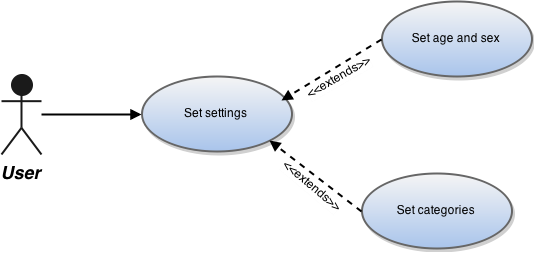
\includegraphics[width=\textwidth]{fig/U3}
	\centering
	\caption{Use case diagram of U3. Set initial settings}
	\label{Fig:U3}
\end{figure}

\begin{table}[hp]
	\renewcommand{\arraystretch}{1.5}
	\centering
	\caption{Textual description of U3. Set initial settings}
	\begin{tabular}[b]{|l | p{13cm}|}\hline
		\textbf{ID} 				& U3									\\\hline
		\textbf{Name} 				& Set initial settings.					\\\hline
		\textbf{Brief description}	& Specify user information to be used for receiving stories. \\\hline
		\textbf{Actors} 			& User									\\\hline
		\textbf{Priority}			& High									\\\hline
		\textbf{Preconditions}		& Application installed, user id received				\\\hline&\\[-2ex]
		\textbf{Basic flow}			& \begin{minipage}{5in}
			\begin{enumerate}[noitemsep]
				\item User is initially asked to fill a form about preferences by the system
					\begin{enumerate}
						\item Personal info: age group and sex
						\item Cultural category preferences
					\end{enumerate}
				\item The system saves information about the user’s preferences
			\end{enumerate}						
		\end{minipage}						\\\hline&\\[-2ex]
		\textbf{Alternate flow}		& \begin{minipage}{5in}
			\begin{enumerate}[noitemsep]
				\item User clicks on settings in order to change preferences
			\end{enumerate}
		\end{minipage}							\\\hline
		\textbf{Postconditions}		& The system has information about the user in order to provide personalized story recommendations.\\\hline
	\end{tabular}
	\label{Tab:U3}
\end{table}

\begin{figure}[hp]
	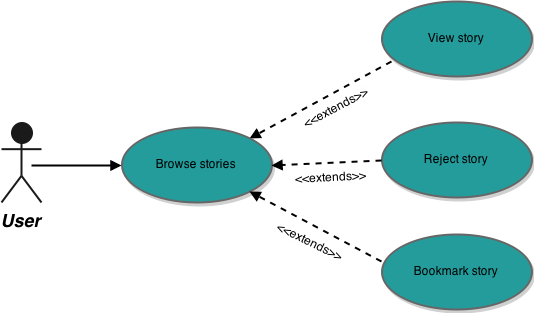
\includegraphics[height=7cm]{fig/U4}
	\centering
	\caption{Use case diagram of U4. Browse recommended stories}
	\label{Fig:U4}
\end{figure}

\begin{table}[hp]
	\renewcommand{\arraystretch}{1.5}
	\centering
	\caption{Textual description of U4. Browse recommended stories}
	\begin{tabular}[b]{|l | l|}\hline
		\textbf{ID} 				& U4									\\\hline
		\textbf{Name} 				& Browse recommended stories.			\\\hline
		\textbf{Brief description}	& User is shown a list of recommended stories to choose from. 		\\\hline
		\textbf{Actors} 			& User									\\\hline
		\textbf{Priority}			& High									\\\hline
		\textbf{Preconditions}		& Preferences already set				\\\hline&\\[-2ex]
		\textbf{Basic flow}			& \begin{minipage}{5in}
			\begin{enumerate}[noitemsep]
				\item User is shown recommended stories including an explanation of why the story was recommended
				\item User does one of the three following actions on a story:
					\begin{enumerate}
						\item Choose to read the story now
						\item Reject the story
						\item Add story to list  
					\end{enumerate}
			\end{enumerate}						
		\end{minipage}						\\\hline&\\[-2ex]
		\textbf{Alternate flow}		& \begin{minipage}{5in}
		\end{minipage}							\\\hline
		\textbf{Postconditions}		& The system has stored information about the choice of the user.\\\hline
	\end{tabular}
	\label{Tab:U4}
\end{table}

\begin{figure}[hp]
	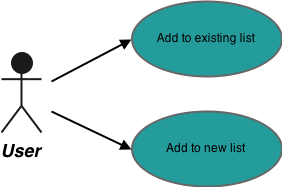
\includegraphics[width=0.5\textwidth]{fig/U5}
	\centering
	\caption{Use case diagram of U5. Add story to list}
	\label{Fig:U5}
\end{figure}

\begin{table}[hp]
	\renewcommand{\arraystretch}{1.5}
	\centering
	\caption{Textual description of U5. Add story to list}
	\begin{tabular}[b]{| p{3.5cm} | p{13cm}|}\hline
		\textbf{ID} 				& U5									\\\hline
		\textbf{Name} 				& Add story to list.					\\\hline
		\textbf{Brief description}	& Put a story in to-read list or user-defined  list. 		\\\hline
		\textbf{Actors} 			& User									\\\hline
		\textbf{Priority}			& Medium								\\\hline
		\textbf{Preconditions}		& User is registered and signed in		\\\hline&\\[-2ex]
		\textbf{Basic flow}			& \begin{minipage}{5in}
			\begin{enumerate}[noitemsep]
				\item User opens a story to read
				\item User clicks the bookmark button in the story and selects the desired collections to put the story in.
				\item Story will be put in the selected list
			\end{enumerate}						
		\end{minipage}						\\\hline&\\[-2ex]
		\textbf{Alternate flow}		& \begin{minipage}{5in}
			\begin{enumerate}[noitemsep]
				\item The desired collection does not exist. The user clicks to add new collection.
			\end{enumerate}
		\end{minipage}							\\\hline
		\textbf{Postconditions}		& Story will be added to and/or removed from various lists according to user's actions\\\hline
	\end{tabular}
	\label{Tab:U5}
\end{table}

\begin{figure}[hp]
	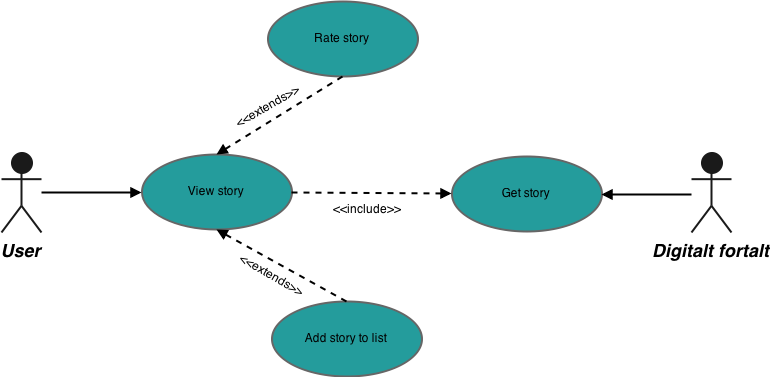
\includegraphics[width=\textwidth]{fig/U6}
	\centering
	\caption{Use case diagram of U6. View story}
	\label{Fig:U6}
\end{figure}

\begin{table}[hp]
	\renewcommand{\arraystretch}{1.5}
	\centering
	\caption{Textual description of U6. View story}
	\begin{tabular}[b]{|p{3.5cm} | p{13cm}|}\hline
		\textbf{ID} 				& U6									\\\hline
		\textbf{Name} 				& View story.							\\\hline
		\textbf{Brief description}	& Display the selected story. 		\\\hline
		\textbf{Actors} 			& User, Digitalt fortalt				\\\hline
		\textbf{Priority}			& High									\\\hline
		\textbf{Preconditions}		& The story has been recommended to the user at some point and is either in the current recommendations list or in one of the other lists			\\\hline&\\[-2ex]
		\textbf{Basic flow}			& \begin{minipage}{5in}
			\begin{enumerate}[noitemsep]
				\item User selects story
				\item Display:
					\begin{enumerate}
						\item The story
						\item Available media formats
						\item Link to story on Digitalt fortalt
					\end{enumerate}
				\item User may select a media format
			\end{enumerate}						
		\end{minipage}						\\\hline&\\[-2ex]
		\textbf{Alternate flow}		& \begin{minipage}{5in}
		\end{minipage}							\\\hline
		\textbf{Postconditions}		& The story is shown according to the user preferences\\\hline
	\end{tabular}
	\label{Tab:U6}
\end{table}

\begin{figure}[hp]
	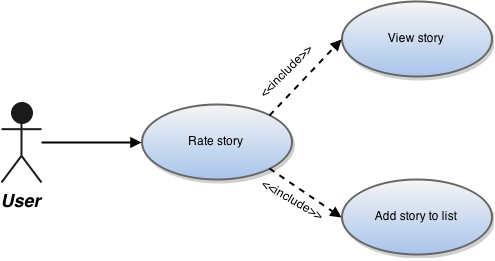
\includegraphics[width=\textwidth]{fig/U7}
	\centering
	\caption{Use case diagram of U7. Rate story}
	\label{Fig:U7}
\end{figure}

\begin{table}[hp]
	\renewcommand{\arraystretch}{1.5}
	\centering
	\caption{Textual description of U7. Rate story}
	\begin{tabular}[b]{|l | l|}\hline
		\textbf{ID} 				& U7									\\\hline
		\textbf{Name} 				& Give feedback / rating.				\\\hline
		\textbf{Brief description}	& Give a rating on a story. 			\\\hline
		\textbf{Actors} 			& User									\\\hline
		\textbf{Priority}			& High									\\\hline
		\textbf{Preconditions}		& User has opened a story for reading	\\\hline&\\[-2ex]
		\textbf{Basic flow}			& \begin{minipage}{5in}
			\begin{enumerate}[noitemsep]
				\item After reading the story,  the user clicks on a rating to give feedback on the story
				\item The system saves the rating
				\item Story will be put in read list
			\end{enumerate}						
		\end{minipage}						\\\hline&\\[-2ex]
		\textbf{Alternate flow}		& \begin{minipage}{5in}
			\begin{enumerate}[noitemsep]
				\item User does not give a rating on the story before closing it
				\item The system reminds the user to rate the story at a later time
			\end{enumerate}
		\end{minipage}							\\\hline
		\textbf{Postconditions}		& The rating of the story from the user is saved\\\hline
	\end{tabular}
	\label{Tab:U7}
\end{table}

\begin{figure}[hp]
	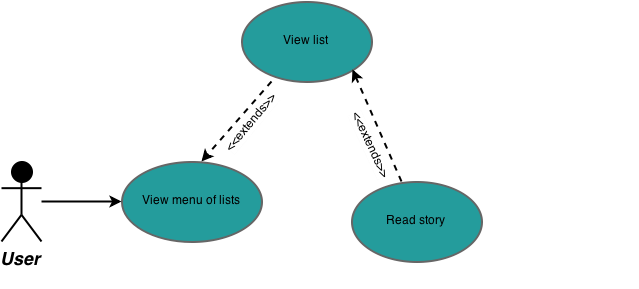
\includegraphics[width=\textwidth]{fig/U8}
	\centering
	\caption{Use case diagram of U8. View list}
	\label{Fig:U8}
\end{figure}

\begin{table}[hp]
	\renewcommand{\arraystretch}{1.5}
	\centering
	\caption{Textual description of U8. View list}
	\begin{tabular}[b]{|l | l|}\hline
		\textbf{ID} 				& U8									\\\hline
		\textbf{Name} 				& View list.							\\\hline
		\textbf{Brief description}	& View list of collected stories (favorites,to-read,tags defined by user). 			\\\hline
		\textbf{Actors} 			& User									\\\hline
		\textbf{Priority}			& Medium								\\\hline
		\textbf{Preconditions}		& User is registered and signed in		\\\hline&\\[-2ex]
		\textbf{Basic flow}			& \begin{minipage}{5in}
			\begin{enumerate}[noitemsep]
				\item User selects list from menu
				\item List of stories shown
			\end{enumerate}						
		\end{minipage}						\\\hline&\\[-2ex]
		\textbf{Alternate flow}		& \begin{minipage}{5in}
			\begin{enumerate}[noitemsep]
				\item No stories found
				\item Display message “No stories found”
			\end{enumerate}
		\end{minipage}							\\\hline
		\textbf{Postconditions}		& User is shown all of the stories collected\\\hline
	\end{tabular}
	\label{Tab:U8}
\end{table}

\begin{figure}[hp]
	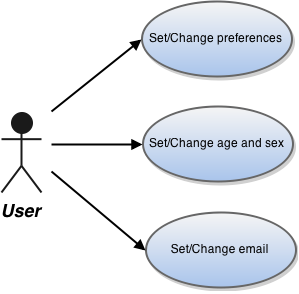
\includegraphics[width=0.5\textwidth]{fig/U9}
	\centering
	\caption{Use case diagram of U9. Specify settings}
	\label{Fig:U9}
\end{figure}

\begin{table}[hp]
	\renewcommand{\arraystretch}{1.5}
	\centering
	\caption{Textual description of U9. Specify settings}
	\begin{tabular}[b]{|l | l|}\hline
		\textbf{ID} 				& U9									\\\hline
		\textbf{Name} 				& Specify settings.						\\\hline
		\textbf{Brief description}	& Specify and change system settings. 	\\\hline
		\textbf{Actors} 			& User									\\\hline
		\textbf{Priority}			& High									\\\hline
		\textbf{Preconditions}		& User is signed in						\\\hline&\\[-2ex]
		\textbf{Basic flow}			& \begin{minipage}{5in}
			\begin{enumerate}[noitemsep]
				\item While logged in, user clicks on settings
				\item User edits the data in settings
					\begin{enumerate}
						\item Category preferences
						\item Age group / sex
						\item User e-mail
					\end{enumerate}
				\item The system saves the new settings
			\end{enumerate}						
		\end{minipage}						\\\hline&\\[-2ex]
		\textbf{Alternate flow}		& \begin{minipage}{5in}
		\end{minipage}							\\\hline
		\textbf{Postconditions}		& Settings are changed and saved\\\hline
	\end{tabular}
	\label{Tab:U9}
\end{table}

\begin{figure}[hp]
	
\includegraphics[width=0.5\textwidth]{fig/U10}
	\centering
	\caption{Use case diagram of U10. Read about app}
	\label{Fig:U10}
\end{figure}

\begin{table}[hp]
	\renewcommand{\arraystretch}{1.5}
	\centering
	\caption{Textual description of U10. Read about app}
	\begin{tabular}[b]{|l | l|}\hline
		\textbf{ID} 				& U10									\\\hline
		\textbf{Name} 				& Read about app.						\\\hline
		\textbf{Brief description}	& Basic info about the application. 	\\\hline
		\textbf{Actors} 			& User									\\\hline
		\textbf{Priority}			& High									\\\hline
		\textbf{Preconditions}		& User is signed in						\\\hline&\\[-2ex]
		\textbf{Basic flow}			& \begin{minipage}{5in}
			\begin{enumerate}[noitemsep]
				\item While logged in, user clicks on settings
				\item User clicks on read about app and is presented with information about the app
			\end{enumerate}						
		\end{minipage}						\\\hline&\\[-2ex]
		\textbf{Alternate flow}		& \begin{minipage}{5in}
		\end{minipage}							\\\hline
		\textbf{Postconditions}		& \\\hline
	\end{tabular}
	\label{Tab:U10}
\end{table}

\pagebreak
\section{Non-functional requirements}
\label{sec:non-functional_requirements}

A general requirement for the project was to use English in all parts related to the documentation of the application, while the language in the application would be Norwegian. Other general requirements concerned the platforms the application should run on. It was decided that it should run on both Android and iOS, and that the design of the application should approach a native feel as much as possible on these platforms.\newline

A quality attribute (QA) is a measurable or testable property of a system that is used to indicate how well the system satisfies the needs of the stakeholders. You can think of a quality attribute as measuring the "goodness" of a product along some dimension of interest to a stakeholder \cite[p.63]{Bass:2012:SAP:2392670}. To make better decisions at a top-level design perspective, and to make better decisions on a component and implementation level, the team wanted the customer to rank each of the quality attributes. The list of QAs and the ranking can be seen in \textbf{Appendix \ref{app:quality_attributes}}. \newline

The ranked list was helpful in choosing the solutions, architecture and patterns that were most in accordance with the customer's vision and needs. In a project with more resources or a more narrow scope there would have been more plans for measuring and quality assure each of the attributes, but this would broaden the scope and workload of a project that were already on a tight schedule\todo{Står det noe om at dette prosjktet opprinnelig var 2?}. Instead this was used as a guideline assisting the development and decision making throughout the project. This was not a decision that was easily compromised but was believed to be one area we could free up some time. With that said, extensive testing and measuring was done to achieve a high quality product\textbf{Appendix \ref{chap:testing}}.\newline


The described quality attributes are the most generic or descriptive for this project \todo{Hva er ment med dette? Omformulere?}. The reader should also keep in mind that there are crossover attributes, e.g.. Maintainability/Testability may increase availability, that could be included in a project of greater scope.

\cleardoublepage


%===================================== CHAPTER 2 Pre-study =================================

\chapter{Pre-study}

This chapter discusses the research that had to be done, and the choices that the team made in relation to choosing development frameworks and technologies. The development process for the project can be found here. The chapter also describes some already existing applications that are similar to this one, and a study about personalization which was a key aspect for this project.

\section{Project assumptions and constraints}
\label{sec:assumptions}

In this section, assumptions and known constraints for the project are addressed. The list of assumptions are details assumed ahead of the documented project requirements, while the constraints specifies matters which would impact the project.

Assumptions on which the planning of the project was based:
\begin{itemize}
	\item Access to an  API for Digitalt fortalt would be provided by the customer.
	\item The customer would give access to a server to deploy the back-end part of the application on.
	\item The frameworks chosen for development had the features needed.
	\item The customer would be available for weekly meetings
	\item Each member of the team would be able to work about 20 hours a week.
	\item The team would meet at least three times a week.
	\item The team would follow the set ground rules as seen in \textbf{Appendix \ref{app:rules_of_engagement}}.
\end{itemize}

Constraints which the team had to work within throughout the project:
\begin{itemize}
\item The deadline for delivering the project was May 30th, and there was no possibility to extend it.
\item The front-end should be developed for both the iOS and Android platforms.
\item The team consisted of 7 people, with little previous experience in mobile application development and no knowledge of personalization algorithms.
\item The application is under the Apache license version 2.0 \cite{HM7}. In summary, this grants copyright and patent rights for users to further distribute it, or distribute a modified version using the same license. It should be clear what the eventual modifications are. The source code can also be used as a part of a closed source project.
\item No budget to pay for software tools.
\end{itemize}

\section{Choice of framework}

As one of the requirements from the customer was that the application should be cross-platform (Android and iOS), a hybrid app was found to be the best option. The alternative would have been to create two separate native apps for both platforms. However, this would have required more work. This would have complicated a delivery within the deadline, especially as the team had little experience with developing for either platform. A hybrid app is a web app made with HTML and JavaScript wrapped in a native shell so that it can be run like a normal native app. This was a big advantage, as the team already had experience with web design. It also makes it possible to make use of the many tools available for web development, and most of the code can be reused for multiple platforms. Bad performance used to be a disadvantage to the hybrid approach, however mobile hardware has improved significantly in the last few years, so this is not a major issue today. The following sections will discuss the advantages and disadvantages of different frameworks that were considered, and explain the final choice for this project. \newline

\textbf{Table \ref{Tab:framework}} below summarizes some of the capabilities and limitations of the various frameworks that were under consideration.

\begin{table}[!h]
	\caption{Framework comparison}
		\begin{tabular}{ | p{6cm} | >{\raggedright}p{3cm} | >{\raggedright}p{3cm} | p{4cm} |}
			\hline
			\textbf{} & \textbf{PhoneGap w/ Ionic} & \textbf{Appcelerator Titanium} & \textbf{PhoneGap w/ Sencha Touch} \\ \hline
			\textbf{Can write a single code that runs on both iOS and Android?} & Yes & No & Yes \\ \hline
			\textbf{Access to native components} & Yes & Yes & Yes \\ \hline
			\textbf{Expected ease of learning and use} & Relatively easy & Difficult & Somewhat difficult \\ \hline
			\textbf{Performance of created application} & Good, AngularJS also provides a performance boost & Very good, as it provides direct access to native components & Acceptable, but not as performance- focused as Ionic. \\ \hline
			\textbf{Debugging} & Easy & Difficult & Easy \\ \hline
			\textbf{Programming language used} & HTML5, CSS, JavaScript with AngularJS & JavaScript & HTML5, CSS,\newline JavaScript \\ \hline
		\end{tabular}
	\label{Tab:framework}
\end{table}

\subsection{PhoneGap}
\label{subsec:phonegap}

PhoneGap is an open-source mobile app framework for native packaging \cite{RA2}. What it does is take in a mobile app consisting of HTML, CSS and JavaScript files, and wrap it in a native shell. It can then be deployed to iOS, Android and Windows 8. It also gives easy access to the native features of the phones (geolocation, notifications, storage, etc.) through different APIs. It is not necessary to think about the native SDKs, as the app will be compiled and built with the newest SDK for the platform.  It is a very popular framework, and there are many plugins created for it that provide additional functionality.

\subsection{Ionic}
\label{subsec:ionic}

Ionic is an open-source UI framework focused on making it easier to create hybrid mobile apps with a native feel \cite{RA1}. It accomplishes this by offering a foundation to build on and UI components based on design patterns and best practices found in native apps. The foundation can be built on and customized with additional HTML, CSS and JavaScript. Part of the foundation is AngularJS, which is a JavaScript framework that extends HTML to make dynamic views in web applications. It gives the app a modular architecture, which means that code can easily be reused for both iOS and Android. A disadvantage is that it is necessary to take time to learn AngularJS in order to take full advantage of Ionic. As Ionic is one of the most popular hybrid mobile frameworks, there exists more learning material about it, and it also has an active user community. Performance is not quite as good on older devices, especially if using large amounts of animations or media.

\subsection{Appcelerator Titanium}

Titanium is a cross-platform Javascript runtime and API framework \cite{RA3}. It currently supports iOS and Android. It offers a JavaScript API which gives access to native UI components and features for the specific platforms, instead of trying to replicate it with CSS or JavaScript like other frameworks. This gives the app a performance advantage, and it is easier to make the interface and interactions feel native. Because the APIs are platform-specific you have to write separate versions of your app for the different platforms. Another disadvantage is that it is difficult to debug as there is no good debugger and Titanium projects cannot be run in Xcode. There would also have been more to learn to be able to use it, as it does not use HTML/CSS.

\subsection{Sencha touch}

Sencha touch is a mobile framework with a large number of UI components and an architecture for the front end \cite{RA4}. Instead of enhancing an HTML file, it generates the document object model (DOM) with JavaScript. The DOM is an interface which creates a representation of the HTML code and allows the developer to manipulate the HTML elements. Sencha touch can be used with PhoneGap, but also has its own native packager. It is harder to learn than Ionic, and the performance is not as good.  It supports the platforms iOS, Android, BlackBerry, and Windows Phone.

\subsection{Conclusion}

The framework combination chosen for this project was Ionic and PhoneGap, as this seemed to fit this project's properties and requirements the best. They are both some of the most popular hybrid frameworks and they are a common combination to use. A prototype can quickly be set up with Ionic, and then iteratively customize it to fit the requirements and create a good user experience. One of the non-functional requirements was that it should be easy to extend the application and to reuse parts of it for other apps. This is fulfilled by Ionic's modular structure. PhoneGap makes it easier to wrap the code in a native iOS and Android shell. This process could also have been done manually, but it requires some knowledge about the native code languages and SDKs. The many plugins available for PhoneGap should also cover the need for use of native features.

\section{Software development process}

The choice of which development process to use in the project was a central decision to be made. The following sections describe the different models that were under consideration by the team, as well as some advantages and disadvantages of each, which influenced the decision of which one to be used for the project. \textbf{Table \ref{Tab:dev-process}} below gives a comparison of some aspects of the various processes that were considered relevant for the project.

\begin{table}[!h]
	\caption{Development process comparison}
	\small
	\begin{adjustbox}{center}
		\begin{tabular}{ | l | l | l | l |}
			\hline
			\textbf{} & \textbf{Scrum} & \textbf{Extreme Programming} & \textbf{Waterfall} \\ \hline
			\textbf{Type of methodology} & Agile & Agile & Plan-driven \\ \hline
			\textbf{Responds well to changes in requirements?} & Yes & Yes & No \\ \hline
			\textbf{Amount of planning needed} & Moderate & Very little & Very much \\ \hline
			\textbf{Level of detail for project plan} & Moderate & Low & High \\ \hline
			\textbf{Customer involvement} & High & High & Low \\ \hline
			\textbf{Frequency of testing} & Continuously & Continuously & Only near the end \\ \hline
			\textbf{Iteration length} & Short & Short & Long \\ \hline
		\end{tabular}
	\end{adjustbox}
	\label{Tab:dev-process}	
\end{table}


\subsection{Waterfall model}
The waterfall model is a plan-driven process with well-defined phases. These phases normally include requirement analysis, system design, implementation, testing, and maintenance \cite[p.30-32]{Sommerville}. It is necessary to finish one phase before starting the next, and due to this, most planning and decisions need to be made at an early stage in the development. As such it is difficult to respond to changes in the requirements. Another issue with this model is that iterations often involve a significant amount of rework and it is normal to postpone some parts of the iterations in order to continue with the later stages of development. This can lead to errors in the system as well as bad design choices.

\subsection{Extreme programming}
Extreme programming is an agile method focused on pushing out new system versions and functionalities rapidly \cite[p.64-72]{Sommerville}. All requirements are written as user scenarios, and before writing the code it is necessary to develop tests for the task. Team members program  in pairs and when the code passes all the tests, it can be integrated into the system.  It is common for a customer representative to take part in the development and make acceptance tests. New system releases are regularly presented to the customer, and this way it becomes easier to cope with changing requirements. Some of the drawbacks of extreme programming include the lack of overall plans for the project. Several documents such as design details and overall report are left out, and it lacks a solid plan for when to implement the various functionalities.


\subsection{Scrum }
\label{sec:scrum}
Scrum is a general agile method with focus on managing iterative development rather than specific technical engineering approaches \cite[p.72-74]{Sommerville}. It also allows for a rapidly changing development environment and close collaboration between the members of a team. To provide this, scrum makes use of phases called sprints, daily scrum meetings, and several types of charts and logs. One of the main challenges for a scrum team is to choose the right amount of work per sprint so that they do not end up with too little or too much work. Scrum has several similarities with extreme programming, such as high involvement of the customer in the development, as well as continuous testing while implementing new functionality.

\subsection{Conclusion}
For this project, the agile software development methodology scrum was used. The project was not very well defined from the beginning, because the customer was not entirely sure of exactly what they wanted. Scrum would be helpful in this regard as it would allow the group to quickly make a simple application which could be tested by the users and customer. Also, an agile process was beneficial as it allowed the team to be flexible and rapidly respond to changes in requirements. The customer requested weekly meetings, and it became a logical decision to make use of scrum to have 1-week  sprints, so there would be definite progress to show between each customer meeting. Since the team was a group of seven, it was impossible to always work together. Because of this, the regular scrum meetings were beneficial to share and discuss progress.


\section{Personalization}
\label{sec:personalization_algorithms}

To provide story recommendations in accordance with each user's interests the content needs to be personalized. Personalization involves using technology to tailor content, to individual users' characteristics or preferences, and to accommodate the differences between individuals. It is a way of meeting the user's needs by making interactions faster and easier, which will hopefully increase user satisfaction and the likelihood of repeat visits. Personalization may be achieved using recommender systems.

\subsection{Recommender systems}

Recommender systems are software tools and techniques that attempts to provide recommendations of items \cite{HM4}. Such systems are simply information filtering systems with the goal of providing suggestions for items to be of use or interest to a user. A few examples of items used in this context are movies, music, books and products in general. Recommender systems typically produce a list of recommendations.  The two most common approaches to produce such a list are content-based filtering and collaborative filtering.

\subsection{Content-based filtering}

Content-based filtering methods are used to find similarities between a user's preferences and the description of an item \cite{HM5}. These algorithms try to recommend items that are similar to items a user has liked in the past or is looking at in the present. Items that a user likes or has interacted with can be seen as a part of the user's profile. Content-based filtering depends on there being much descriptive data available on the items. To find items to recommend, items are compared against a user's profile, and recommendations are given based on how well they match the profile. User feedback, usually in the form of rating or a like or dislike button, can be used to assign weights to certain attributes. By using user feedback and weighting it is possible to give more accurate recommendations. \cite{HM4}

\subsection{Collaborative filtering}

Collaborative filtering is based on collecting and comparing information on users' behavior, activities or preferences and to recommend items based on a user's similarity to other users \cite{HM6}. This approach tries to predict what a user will like based on what similar users have liked. Collaborative filtering assumes that users who have agreed in the past will agree in the future, and that they will like similar items as they liked in the past. These methods often suffer from the problems; cold start and sparsity. Collaborative filtering often requires a large amount of existing data on users to be able to make accurate recommendations. The cold start problem is the absence of such data at the beginning of a project. The sparsity problem is that collaborative systems are dependent on having many active users to properly distribute ratings across all the items in the system. However, most active users have only rated a few items in the overall database, which means that even the most popular items have very few ratings. The greatest strength of these techniques is that they are independent of any documented representation, e.g. textual descriptions and subject-tags, of the objects being recommended and work well for objects that are difficult to define such as music and movies.\cite{HM4}

\section{Existing solutions}
\label{sec:existing_solutions}

Among the previous work there has been developed applications through the TagCloud project. This section evaluate two of those applications, namely \textit{stedr} and \textit{Cooltura}. Both of these applications presents stories regarding cultural heritage. Since this project also included personalization, an evaluation was additionally performed on the application \textit{Magic Tate Ball}. This application was chosen because the customer mentioned this as a possible inspiration for the current project. \newline

These three applications were evaluated using the following criteria:
\begin{itemize}
\item Content. Does the application provide satisfying content or is something lacking?
\item Usability. Usability concerns how easy it is for the user to accomplish a task. (see \textbf{Section \ref{sec:non-functional_requirements}} for a more elaborate definition). The evaluation here draw on Jacob Nielsen’s ten usability heuristics as defined in \cite{AS3}.  
\item Personalization. To what extent does the application provide the user with the opportunity for individualized content?
\end{itemize}

The main findings in the evaluation are summarized in \textbf{Table \ref{Tab:existing_solutions}}.

\begin{table}[t]
	\caption{Summary of the main findings in the evaluation of existing solutions}
	\begin{tabular}[b]{ | p{2.7cm} | >{\raggedright}p{4.3cm} | >{\raggedright}p{4.3cm} | p{4.3cm} |}
		\hline
		\textbf{} & \textbf{stedr} & \textbf{Cooltura} & \textbf{Magic Tate Ball} \\ \hline
		\textbf{Content} & Stories related to places in Trondheim & Stories from three places, including Trondheim & Artworks and some information about them \\ \hline
		\textbf{Usability} & 
			- Requires knowledge of the location to find places on map \newline
			- The picture occupies much of the space in the place and story view \newline
			- Good help site\newline
			- Clear and consistent language 
			& 
			- List of locations is easier to navigate than a map and does not require knowledge of the exact location of the places\newline
			- Picture is dynamic and makes room for the relevant information to the user when scrolling \newline
			- Lacks a help site
			&  
			- Two options for starting the and for browsing the artworks accommodates different user groups \newline
			- Visibility of system status when processing 		
			 \\ \hline
		\textbf{Personalization} & Does not provide any personalization feature & Not implemented in the tested version & Provide personalization using different input parameters.  \\ \hline
	\end{tabular}
	\label{Tab:existing_solutions}
\end{table}

\subsection{stedr}
\label{subsec:stedr}

The stedr application was developed by students as a prototype to test some research hypothesis. Content was not the primary focus in the application and thus consists mainly of stories related to places in Trondheim. A possible problem in the application is finding the place the user is looking for since the main view consist of a map with markers representing each available place. In order to know which place each marker represents the user have to click on the marker, which means that the user might click on multiple markers do find the desired place. \newline 

The place view in stedr can be seen in \textbf{Figure \ref{Fig:stedr_screenshot}}. To see all the content, one might have to scroll down. The main picture is static when scrolling, occupying the upper half of the screen, which is also the case when viewing a specific story in the story view. It might be argued that Nielsen's heuristic of aesthetic and minimalist design in case of scrolling is violated as the picture's importance in the dialogue is less important than the space it occupies suggest. \newline

\begin{figure}[h]
	\centering
	\begin{subfigure}[t]{0.3\textwidth}
		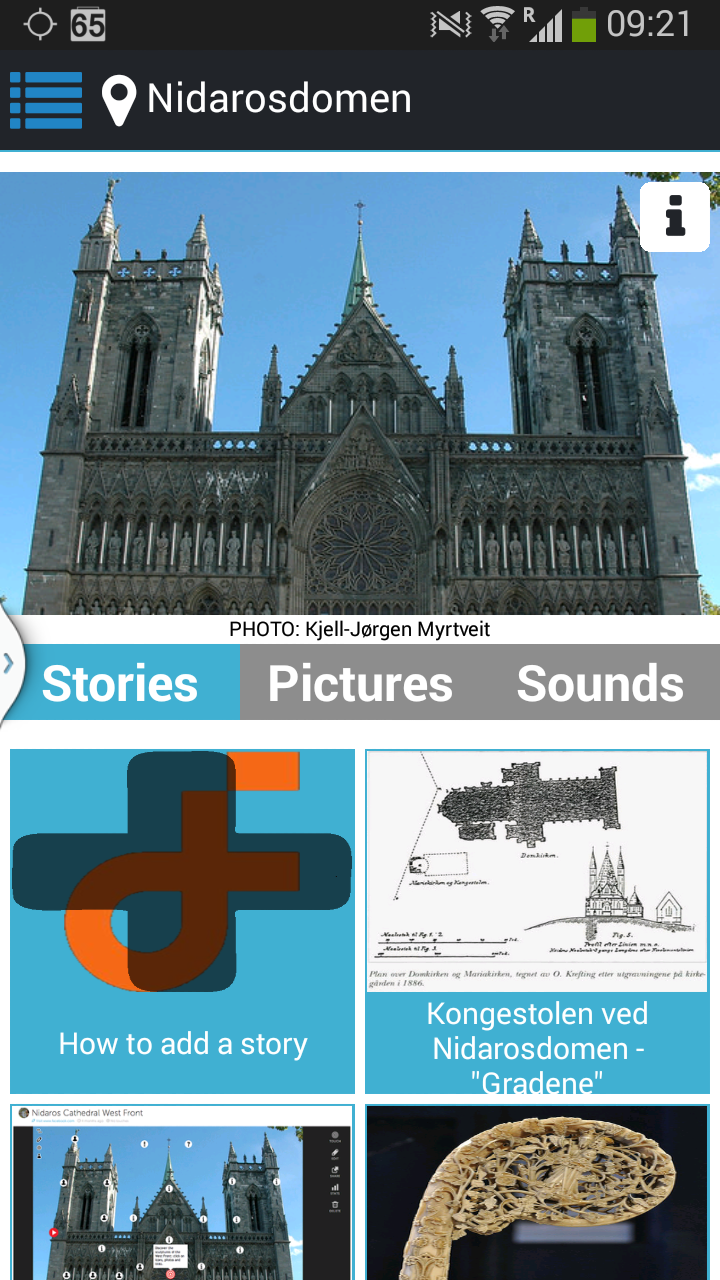
\includegraphics[width=\textwidth]{fig/stedr_screenshot}
		\caption{A screenshot from stedr showing the available options for one place}
		\label{Fig:stedr_screenshot}
	\end{subfigure}
	\hspace{0.5cm}
	\begin{subfigure}[t]{0.3\textwidth}
		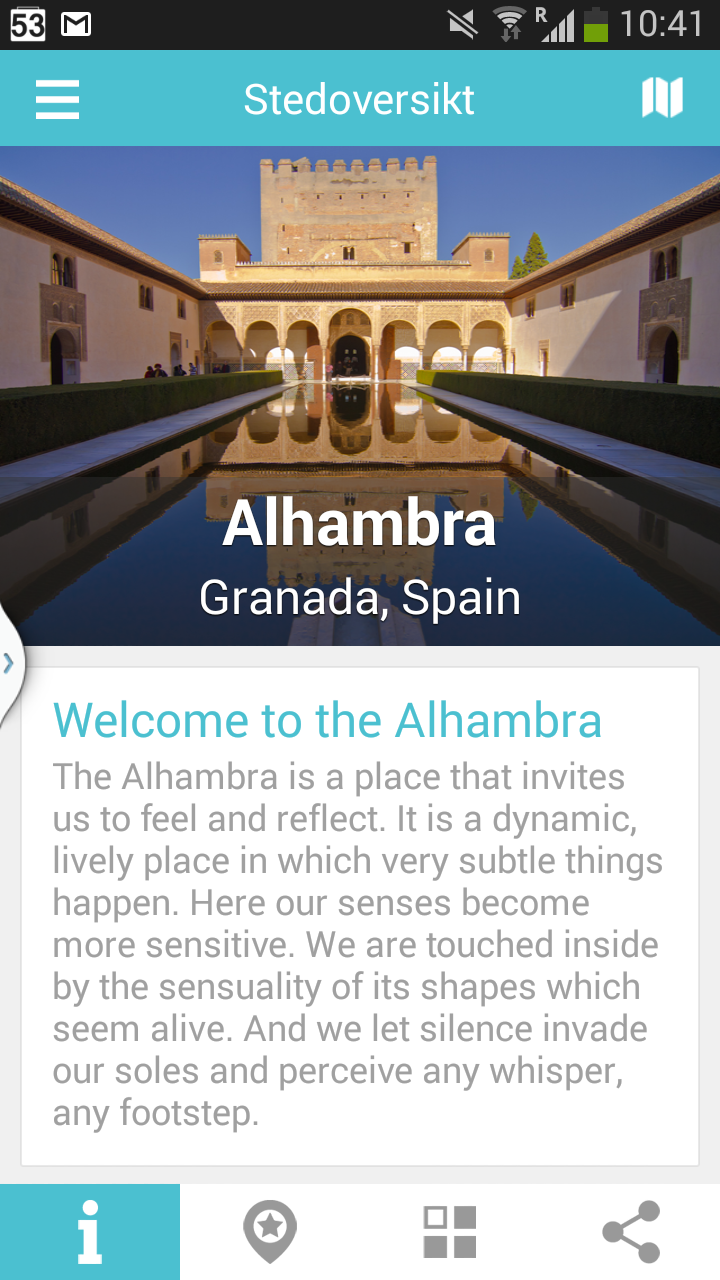
\includegraphics[width=\textwidth]{fig/cooltura_screenshot2}
		\caption{A screenshot of Cooltura showing the view for one particular place}
		\label{Fig:cooltura_screenshot2}	
	\end{subfigure}	
	\hspace{0.5cm}	
	\begin{subfigure}[t]{0.3\textwidth}
		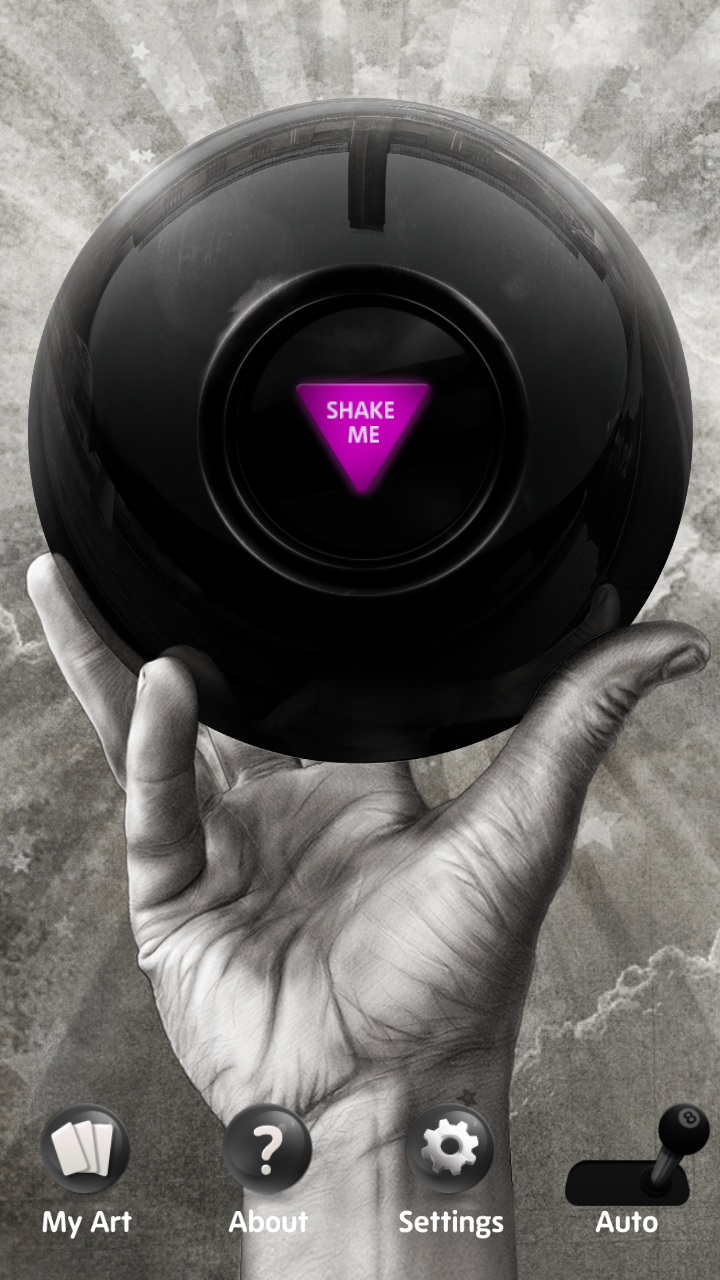
\includegraphics[width=\textwidth]{fig/tateball_screenshot}
		\caption{A screenshot of the main view of Magic Tate Ball}
		\label{Fig:tateball_screenshot}		
	\end{subfigure}	
	\caption{Place views in stedr and Cooltura and the main view of Magic Tate Ball}
\end{figure}

The application provides a help site which gives a thorough guide to the user on how to accomplish tasks. This is in accordance with Nielsen's heuristic of help and documentation. The application also helps the user when errors occur, for instance by offering the user a refresh opportunity when the map does not load the places. The language used in the application is both user-centered and consistent, avoiding misunderstandings and making it easy for the user to understand what different actions entails. \newline

The application does not provide any personalization feature, which is the main difference between stedr and our application. The customer’s motivation for creating an entirely new application instead of expanding stedr was mainly because they wished to test personalization systems on users, and thus needed an application focused mainly around the personalization aspect. In addition, it became possible to access a larger number of stories than stedr currently does. 

\subsection{Cooltura}

Cooltura is another application developed under the TagCloud umbrella. The version of Cooltura evaluated here is a demo version, so more developed versions of the application may include more functionality and address some of the issues discussed here. \newline

The content is somewhat similar to stedr, with respect to the places and the stories available. In fact, when clicking to view stories in Cooltura one is directed to the stedr app. Cooltura does not use a map like stedr, but instead a list of available locations. This makes it far easier for the user to navigate to the right place, especially since the selection is quite limited. When viewing a specific place on Cooltura the user gets a view with a main picture and some text describing the place as seen in \textbf{Figure \ref{Fig:cooltura_screenshot2}}. Like in stedr the user can scroll down to see more content, but unlike stedr the main picture is not static, that is, the user see less and less of it as it scrolls down. This is more in accordance with Nielsen's point of aesthetic and minimalist design, where less relevant information fills up less space in the user interface. The same is true for the view for a specific tourist attraction. The application does not provide any help site, but the possible user actions are quite few and similar (most of them are about navigating to the desired place), so this might not be a problem.\newline

It appears that the application intends to make use of personalization, but this is not implemented at the time of writing this report \cite{AS4}. The “Anbefalte steder”-view in Cooltura now list every place added in the application (which is three different places), but the heading suggests that personalization is planned for. 

\subsection{Magic Tate Ball}

Magic Tate Ball is an application that presents the user with an artwork based on the input parameters: date, time-of-day, geographical location, live weather data and ambient noise levels \cite{AS5}. The content in the application is the artwork, a description of the artwork and an explanation of why the artwork was chosen. Personalization is the main selling point of Magic Tate Ball. The application uses the input parameters to give the user some control of what content is presented as the user can turn each of these parameters on and off. Even though the application provides an explanation to why an artwork was chosen, how it was chosen remains in the dark (e.g. how to know which input parameter was emphasized in the personalization).\newline


The main task in the application is to be presented with an artwork. This is done by shaking the phone or by clicking a button in the center of the magic ball, see \textbf{Figure \ref{Fig:tateball_screenshot}} for a screenshot of this. Another task is to browse all artworks presented to the user, which is done by swiping or clicking on arrows. Providing these two options makes it easy to for different types of users, those accustomed to swiping and those who are not. When the application is processing to come up with an artwork to present to the user, it shows the user what the input parameters are. This is in accordance with Nielsen's heuristics on visibility of system status. \newline

\cleardoublepage
%===================================== CHAPTER 7 Tools =================================

\chapter{Tools}

This section briefly describes all the tools used for this project, which includes development tools, communication tools and any additional tools.

\section{Development tools}

\subsection{Front-end}
\begin{itemize}
	\item Ionic \cite{es1} - Ionic is a front-end UI framework designed to assist the development of hybrid mobile applications. By using this framework it became easy for the team to speed up the design of the interface and test the application both on computers and devices. More details about Ionic can be found in \textbf{Section \ref{subsec:ionic}}
	\item PhoneGap (Apache Cordova) \cite{RA2} - PhoneGap is a framework that enables software developers to automatically wrap HTML5, CSS and JavaScript code into platform-specific code that can run on devices such as iOS and Android phones and tablets. The Ionic framework is based on using PhoneGap for compiling its code. More details about PhoneGap can be found in \textbf{Section \ref{subsec:phonegap}}
	\item Android Studio \cite{es22} - Android Studio is the official IDE for Android application development, it was necessary to have this installed in order to develop our application on android devices. It also provided a way to install various plugins that were useful or needed for the project.
	\item Node.js \cite{es23} - Node.js is a platform built on Chrome's JavaScript runtime for easily building fast, scalable network applications. This was another tool that was necessary to install, because PhoneGap is built on it. First released in May of 2009, Node.js has been gaining much popularity as a server-side platform. 
	\item Gulp.js \cite{es24} - Gulp is a build tool that is used as a part of PhoneGap in order to automate many common tasks, such as build processes and plugin handling.
	\item Sass \cite{es25} - Sass is an extension to CSS which adds functionality such as being able to use variables, nested rules and inline imports. Sass helps keep stylesheets organized, and is fully compatible with regular CSS syntax. Sass is the preferred tool for handling stylesheets in Ionic.
	\item Proto.io \cite{protoIO} - This a prototyping framework aimed for mobile apps, and it allowed the team to make very quick and functional prototypes that were used for user testing, both by the team and by the customer. When discussing design solutions, it was much faster and simpler to make revisions to the prototype than it would be to redesign the application itself. 
	\item Balsamiq \cite{es3} - Wireframing and mock-up tool which was used to create early mock-ups of the different user interface views. This was used because it allowed the team to quickly make wireframes for the interfaces, and it gives a more professional look than by  just making paper prototypes.
	\item Icomoon \cite{es4} - This is an application with the purpose of generating an icon font from svg files that you upload to it. You can also resize, adjust positions, and set default pixel sizes for the icons. The application turns all the icons into crisp-looking and easy scalable icons. It also automatically generates the HTML and CSS code which you can use to integrate the code into your own application. In this project, Icomoon was used to make the category icons that show the various categories on each story
	\item FontForge \cite{es5} - After creating an icon font with Icomoon, FontForge was used to make manual adjustments to the icons themselves. FontForge is an editor with many advanced options for giving icons a smoother look and symmetry.
	\item Karma \cite{KF3} - Karma is a test runner for AngularJS. With Karma it is possible to write JavaScript tests and run it in different browsers on both desktops and mobile phones. It is easy to run a test for every integration you make. More details about how Karma was used in this project can be found in \textbf{Section \ref{sec:unit_testing}}	
\end{itemize}

\subsection{Back-end}
\begin{itemize}
	\item Docker \cite{EHW2} - Docker is an open platform that provides the possibility for system developers to build their application and deploy it to other computers or servers, which can then run the same application, unchanged. The motivation for using Docker was mainly so the team could run the developed application on SINTEF's own server. More details about Docker is described in \textbf{Section \ref{subsec:docker}}
	\item MySQL \cite{es8} - MySQL is one of the most widely used open source databases. It has many advantages when it comes to scalability and flexibility, and it is well suited for many types of application development. More details about this project's database and its design can be found in \textbf{Section \ref{sec:database_design}}
	\item Digitalt musem API \cite{digitaltMuseum} - The source of the stories in the application was Digitalt Fortalt, and in order to access these it was necessary to use Digitalt museum's API. The API is documented on its website and was incorporated into the project's database. Details about the API and the use of it can be found in \textbf{Section \ref{sec:harvesting}}
	\item PHPUnit \cite{KF2} - PHPUnit is a framework for writing and performing unit tests on PHP code. More details about how PHPUnit was used in this project can be found in \textbf{Section \ref{sec:unit_testing}}
	\item JUnit \cite{jUnit} - JUnit is a framework for doing unit testing in Java. 
	\item DbUnit \cite{dbUnit} - DbUnit is an extension of JUnit that can be used to test methods accessing a database. Among its advantages is the ability to put the database in a known state before each test, which gives the tester control over what to expect as results of tests that change the contents of the database.
	\item Mahout \cite{as9} \todo{Mahout krever at man har Apache Commons Math, Guava-libraries og slf4j. Skal disse nevnes?} - Mahout is a project that provides scalable machine learning algorithms. Mahout is primarily focused on algorithms for collaborative filtering, clustering and classification. How Mahout has been used in this project is described in \textbf{Section \ref{sec:personalization_how}}.
\end{itemize}

\section{Communication tools}
\label{sec:communication tools}

\begin{itemize}
	\item Google Drive \cite{es10} - Used for creating and sharing documents with the whole group, as well as editing shared documents in real-time. it also made it possible to share all files, whether it was images/diagrams/spreadsheets, or anything else. That was why the team decided to use this as a good solution for sharing all documentation.
	\item Dropbox \cite{es11} - Used to share documents between the group and the customer. This tool was used upon request by the customer.
	\item Facebook \cite{es13} - Used for discussions and notifications of various things such as meeting times. This was used because Facebook is something everyone was already familiar with, and something that most of the team members use on a regular basis, so messages would be quickly noticed.
	\item Trello \cite{es15} - Task management application, this was a handy way to quickly see what needs to be done and what has already been completed, similar to a scrum task board . Because of this, the team found it to be a good tool to use, as it speeds up the process of managing work tasks and gave a better overview of the progress.
\end{itemize}

\section{Additional tools}
\label{sec:additional_tools}

\begin{itemize}
	\item GitHub \cite{es12} - Used for making a code repository to be shared by the group while developing the system. The customer requested the use of GitHub, and it was also used because it seemed like the easiest way to share and implement code, as well as sharing the code with the customer.
	\item Draw.io \cite{es14} - This tool was the primary way of making diagrams and models, such as use-cases and WBS chart. This tool was chosen for this because it provides a lot of templates for different types of graphs, and as everyone uses the same tool for all diagrams the report achieves a consistent style for every diagram.
	\item Ganttify \cite{RG1} - Converting Trello boards into Gantt Charts, makes the process of creating a gantt chart and milstone plan easier and faster.
\end{itemize}

\cleardoublepage
%===================================== CHAPTER 3 Project management =================================

\chapter{Project management}

The following chapter describes planning the progress of the project, managing resources, controlling potential risks and assure quality of the project. The project management includes a delegation of work tasks and responsibilities, risk management, a work breakdown, time management and quality assurance.

\section{Risk management}

Risk management includes planning and handling all the various potential risks to the project.

The risk analysis contains a list of possible occurrences that could be harmful to the project. Provided for each risk is a short description, an estimated likelihood that the risk will happen, an estimated impact to the project if it happens, the importance of the risk, a preventive action to try to avoid the problem and a remedial action if the problem were to occur. Likelihood and impact estimates were rated on a scale from 1 to 9, with 9 being the highest, and the importance was calculated by multiplying likelihood with impact. The risk list is sorted by the importance value, thus the risk to be most aware of at each stage of the development process was at the top of the list.
 Risks were updated regularly and changes were made when we discovered new issues that needed to be managed. 

 \textbf{Table \ref{Tab:riskexample}} describes four of the most important risks in the risk analysis. The complete risk analysis is located in the \textbf{Appendix A \ref{Tab:risklist}}.


\begin{center}
	\begin{longtable}{ | p{3.5cm} | p{2cm} | p{1.5cm} | p{2cm} | p{3.5cm} | p{3.5cm}|}
		
		\caption[Risk list example]{Risk list example } \label{Tab:riskexample}\\
		\hline
		\textbf{Description} & \textbf{Likelihood(1-9)} & \textbf{Impact(1-9)} & \textbf{Importance (Likelihood * Impact)} & \textbf{Preventive action} & \textbf{Remedial action}\\ \hline
		
		The group does not receive quality feedback from supervisor & 6 & 6 & 36 & Be prepared for supervisor meetings. Prepare concrete questions and discuss issues with supervisor & Ask qualified aquaintances to read and give feedback on the report. \\ \hline
		
		Project complexity / Project too difficult & 5 & 5 & 25 & Do not plan many complicated tasks & Downgrade demands \\ \hline  
		
		Poor communication within the group leading to misunderstandings and doubts about the progress of the project & 4 & 6 & 24 & Write meeting minutes to document decisions. Have frequent meetings where every team member explains what they have done and what they are planning to do & Make a group decision to solve the misunderstanding \\ \hline

	\end{longtable}
\end{center}


\section{Scrum team and roles}
\label{sec:scrum_team_and_roles}

The role delegation in the team is detailed in \textbf{Table \ref{Tab:roles}}. The delegation of roles was primarily based on personal interest and motivation. The tasks were divided up into main responsibility areas for back end and front end before assigning people to each one. However, this was only  a guideline for main responsibilities, and the group members had to be flexible and work on some tasks outside of their main areas.

\begin{table}[!h]
	\small
	\centering
		\begin{tabular}{ | p{3.7cm} | p{2.8cm} | p{10.5cm} |}
			\hline
			\textbf{Role} & \textbf{Responsible} & \textbf{Details} \\ \hline
			
			\textbf{Product Owner} & Jacqueline Floch (SINTEF) & \\ \hline
			
			\textbf{Main back end staff} & Hanne Marie, Eivind, Kjersti, Audun & \\ \hline
			
			Interaction between server modules & Hanne Marie & This involves making the different server components communicate and work together, such as the database, personalization module, Docker file, etc. \\ \hline
			
			Personalization & Eivind & Involves the procedure for taking a user’s context information and preferences, and based on this choose which stories to present to the user. Also involves collaborative filtering to select stories for a user based on the preferences of other users. \\ \hline
			
			Test responsible & Kjersti & Involves creating a test plan for each kind of test (unit, usability, integration, etc.) and documenting the results, as well as assuring test quality and that the tests are actually conducted properly. \\ \hline
			
			Database Manager & Audun & Involves setting up and managing the database. Manage which elements to save in the database and how to present the data upon request. \\ \hline
			
			\textbf{Main Front end staff} & Ragnhild, Roar, Espen & \\ \hline
			
			iOS responsible & Ragnhild & Involves developing and giving the app a look and design that feels intuitive and follows design conventions according to iOS systems. This is both on a technical and design level. \\ \hline
			
			Android responsible & Roar & Involves developing and giving the app a look and design that feels intuitive and follows design conventions according to Android systems. This is both on a  technical and design level. \\ \hline
			
			Framework responsible & Espen & Involves developing various parts of the UI, and researching the framework to ensure that the front end design can be made and is made according to the team’s and customer’s expectations. \\ \hline
			
			\textbf{Additional roles} & Roar, Kjersti, Espen & \\ \hline
			
			Scrum Master & Roar & Project leader, responsible for arranging meetings, delegating work tasks, and overseeing the general progress of the project. Facilitate the communication and cooperation between the group members. \\ \hline
			
			Customer relations & Kjersti & This includes all communication with the customer, as well as other authorities that are a part of the project. \\ \hline
			
			Report management & Espen & This involves overseeing the report work and ensuring that all components of the report are in place.  Deliver the report within deadlines and make changes as needed and in accordance with advice from supervisor. \\ \hline
		\end{tabular}
	\caption{Role delegation}
	\label{Tab:roles}
\end{table}

\section{Work breakdown structure}

A work breakdown structure is a decomposition of the project and its goal is to break down each part of the development process into manageable parts to ease the planning and execution of the development. Each element in the diagram can be a product, data, service or a combination of the three. One of the benefits of detailing a project this way appears when doing cost estimation and scheduling the team around the project (i.e. should ease the project planning and help allocate the team’s resources).\newline

The work breakdown structure should show a hierarchical decomposition of the project phases and its components. Each main phase is at a top-level and will outline the generic parts of the software development processes. The way the WBS (Work Breakdown Structure) is developed is by starting with the end objective and subdividing each main part into manageable components in terms of size, complexity and duration. Each sub objective is to follow the 80 hour rule. This means that a subtask is not to exceed 80 hours in magnitude.  The WBS for this project is shown below in \textbf{Fig \ref{Fig:wbs}}

\begin{figure}[h!]
	\centering
	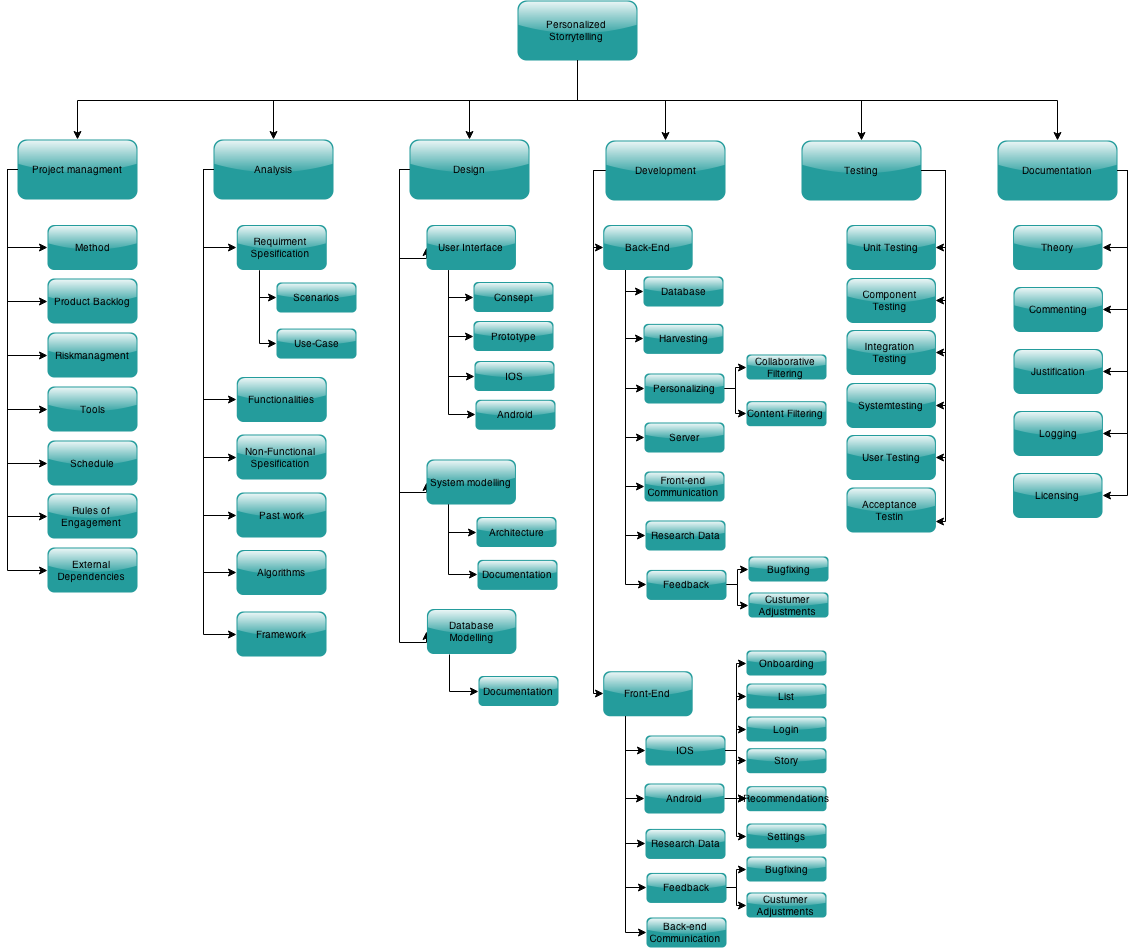
\includegraphics[width=\textwidth]{fig/wbs}
	\caption{Work breakdown structure}
	\label{Fig:wbs}
\end{figure}

\section{Project milestone plan}
\label{sec:milestone_plan}

TODO: put the Gantt and burndown chart here and describe the time/sprint planning.\newline

Milestones are used as tools in project management to give the team some clear and specific goals to work towards as the project timeline moves ahead. There are several milestones throughout the project, some are large milestones like; alpha and beta versions of the software. There are also milestones related to the project report, like the midterm submitting. and final delivery. Milestones can add some value to the project scheduling when used in the right manner and when setting realistic goals. Components that are important for the milestone plan are; key dates, key deadlines and external deliveries.  The team used a combined Gantt chart with milestones noted for better visualization, and to better allocate resources for meeting the milestone goals.\newline

The planned deliveries to the customer is the following dates. 
\begin{itemize}
\item 20.02.15 First prototype on paper
\item 27.02.15 Second prototype presented in proto.io[KF2]
\item 17.03.15 First working software(alpha-version)
\item 10.04.15 Second working software(beta-version) 
\item 01.05.15 Final product
\end{itemize}

\section{Quality assurance}

According to Sommerville quality assurance is “the definition of processes and standards that should lead to high-quality products and the introduction of quality processes into the manufacturing process” [AS6]. In large systems, designed to be used in a long term perspective, quality documentation is important. However, in this project a small system was developed and Sommerville notes that a more informal approach can then be applied, focusing on “establishing a quality culture” [AS6] within the development team.\newline

Therefore, this section will describe three features considered important by the group to establish such a quality culture, and thus improving the quality of the product, namely group interaction, version controlling, and interaction with the customer. Risk management and testing are also important aspects of quality assurance, and these are discussed in separate chapters(see \textbf{Chapter \ref{chap:risk_management}} for risk management and \textbf{Chapter \ref{chap:testing}} for testing). 

\subsection{Group interaction}

As was noted in \textbf{Section \ref{sec:scrum}} (Pre-study - Scrum) an important part of the scrum methodology is the close collaboration between the team members. Scrum provide some events to enhance this collaboration, for instance the daily scrum meetings, and some artifacts, such as the sprint backlog. These features of scrum was used by the group and created a framework for the process development. However, scrum does not define how the group should interact, and the group interaction consisted of more than the methods provided by scrum, for instance when doing sessions of collaborative work.\newline

In order to ensure that the scrum events and the interaction external to these events would create the desired quality culture, the team discussed and agreed upon some basic rules of engagement for the project. These rules specified how the team should create a quality process in order to create a quality product, for instance by setting ground rules for communication between the group members. The tools described in \textbf{Section \ref{sec:communication tools}} (Tools-communication tools) were used to facilitate the implementation of the rules. In addition, meeting minutes from every meeting was made so that every group member would be aware of the status of the project even if they were not present at the meeting.\newline

The division of the group described in \textbf{Section \ref{sec:scrum_team_and_roles}} (Project management - Scrum team and roles) meant that a member of the front end part would have more detailed information about what other front end developers were doing than what individual members of the back end part were doing, and vice versa. However, when important decisions were to be made in one part of the project or important problems had to be solved, both parts would be involved in the discussion, even if the decision did not affect their part of the project directly. An example of such a decision was the choice of colours to use in the user interface.

\subsection{Git and version controlling}

The code for this project is hosted by GitHub, a tool described in \textbf{Section \ref{sec:additional_tools}} (Additional tools). GitHub uses the version control system git, which makes development easier by allowing multiple local branches and thereby giving users the opportunity to try out code before committing them to the master branch. The master branch is the main branch and should only include stable code. The group chose to create two repositories, one for the back end part of the project and one for the front end part since the group also was divided in this way. Doing it this way made keeping track of branches and issues on Github clearer since these often would be at a level of detail only relevant to the developers in that part of the project. 

\subsection{Customer interaction}

In \textbf{Section \ref{sec:scrum}} (Pre-study-scrum) it was noted that the project was not clearly defined at the start. This meant that good customer interaction was critical, so that the group and the customer would be in agreement of what was expected of the end product. Communication with the customer was done by weekly meetings (some weeks were skipped in the later part of the project period because there were no issues to discuss), mail and by a shared Dropbox folder. In addition, the customer had access to the code on GitHub. \newline

A couple of days before the weekly meetings, the group would add a meeting agenda to the Dropbox folder. This was done to improve the structure of the meeting and to give the participants time to consider the issues on the agenda, which in turn should increase the benefits of the meeting and increase the likelihood of making decisions. Making decisions and coming to an agreement with the customer on key issues was considered important to push the project forward. After the meeting the group would add a minute of the meeting to Dropbox, so that the customer would know if all the participants had a similar understanding of the issues discussed and the decisions made. Communication by mail was mainly used to rescheduling of meetings and by the customer to give additional information to the group. 



\cleardoublepage
%===================================== CHAPTER 6 Design and architecture =================================

\chapter{Design and architecture}

To get a brief overview of the complete product and its required parts, the design and architecture are presented in this chapter. This is not meant to give a complete understanding of the system, but rather an overview on how the different parts of the product work together to give a pleasant user experience.

\section{Architecture}

The overall architectural design of the system was made to achieve a rough mapping of what needed to be done in terms of actual programming. The architecture focuses heavily on interactions between the different instances in the systems without going into the specific details on how this is done. To illustrate the architecture, two different views were created. One showing only the components, and the other showing the processes in the different components. The overall system structure can be seen in \textbf{Figure \ref{Fig:system_structure}}, this shows the four different components and how they interact. As shown in this diagram, the system is created as a client-server model, where the mobile application constitutes the client, which communicates with the PHP back-end server. The server is connected to a database, and Digitalt fortalt provides an API to retrieve stories from.\newline

The \textbf{Figure \ref{Fig:architecture}} shows a diagram presenting the architecture for the application. As seen in the legend, the square boxes represent individual components or processes. The boxes with oval corners represent compound processes or larger parts. These are mainly shown because they give an overview of which processes belong to and will be performed by which part of the system. Double lined boxes are external sources which provide an API. Lastly, arrows indicate information flow.

\begin{figure}[h!]
	\centering
	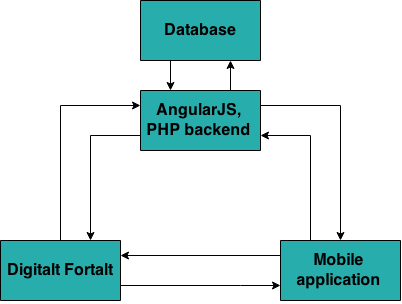
\includegraphics[width=0.5\textwidth]{fig/system_structure}
	\caption{Diagram of the overall system structure for this project.}
	\label{Fig:system_structure}
\end{figure}

It is a difficult task to model a whole system in an accurate way, and while the architecture diagram shows an overlook, it can not give much insight into the complexity of each process. This is further complicated by the fact that in the startup phase of the project there are a great number of unknowns. Both complexity and requirements are subject to change. As such, the diagram should only be used as a guide for understanding the composition of the complete system.

\begin{figure}[h!]
	\begin{center}
		\advance\leftskip-3cm
		\advance\rightskip-3cm
		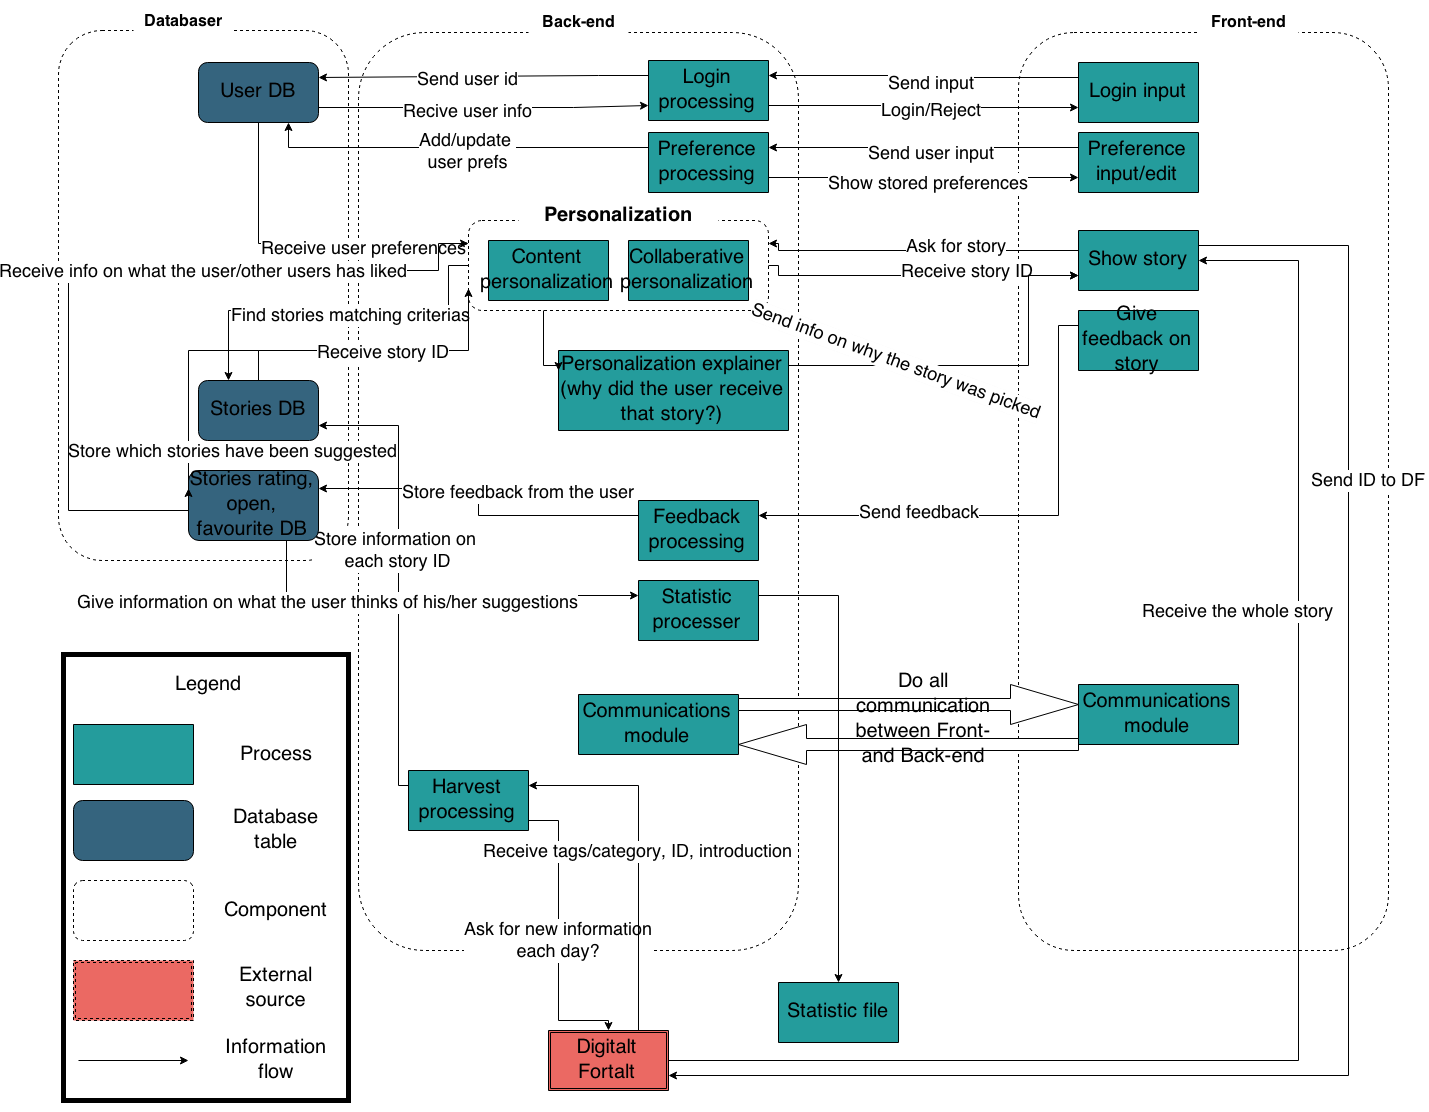
\includegraphics[keepaspectratio=true,scale=0.4]{fig/architecture}
		\caption{Diagram of the architecture for this project.}
		\label{Fig:architecture}
	\end{center}
	\end{figure}

\section{Front-end structure}
\label{sec:frontend_structure}
The front-end of the application was designed by using Ionic and AngularJS, and this section will describe how a system made in AngularJS is structured.

AngularJS provides templates to create systems based on a Model-View-Controller(MVC) architecture, and also provides a variety of components to assist in making the programming more effective and speeding up the application. It is essentially another layer of abstraction above writing regular JavaScript. These are some of the main concepts that are used to create an Angular application:

\begin{description}
	\item[Model] \hfill \\ 
	Manages all the data that can be interacted with by the user. The model also keeps the views up to date and can be manipulated by controllers.
	
	\item[View] \hfill \\ 
	The interfaces that the user can see. This means some form of visual representation of the model.
	
	\item[Controller] \hfill \\ 
	The logic and behavior of the views. The controllers also make changes the model.
	
	\item[Directive] \hfill \\ 
	Special functionality applied to the DOM elements, you can create your own directives as well as use the numerous ones provided by AngularJS itself. In "Vettu hva?", several of these were used, such as directives that call on some function when DOM elements are clicked on, or directives that show or hide parts of the DOM based on some condition.
	
	\item[Module] \hfill \\ 
	A module encapsulates a part of the application. Instead of having a single "main" function that holds the application together, Angular applications normally have multiple modules that work together. The benefit of this is that the application is decomposed into logical parts that can be reused, loaded, and tested in any order. In "Vettu hva?", each controller is its own module. The part of the program that communicates with the back-end is also encapsulated in a module. Furthermore, there is a module that starts up the application and binds together views and controller into different states.
	
	\item[Scope] \hfill \\ 
	The scope contains all the elements that the application currently has access too. It can be viewed as a container that stores the current model, and so if a controller or directive is going to modify or access the model, this has to be done by using the scope.
	
	\item[Service] \hfill \\ 
	A service contains "global" logic that is accessible to the entire application. In "Vettu hva?", this is used in the module that contains the communication with the back-end. This module has three different services, which respectively gives the application access to user data, story data, and requests from front-end to back-end.
\end{description}

\section{User interface}

\todo{Introduksjon}

\begin{figure}[h!]
	\centering
	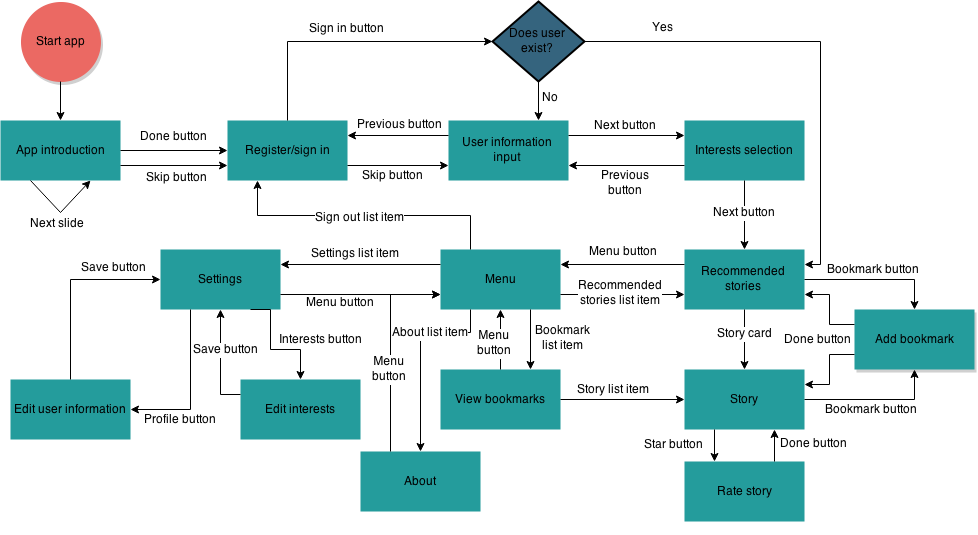
\includegraphics[width=\textwidth]{fig/flow_diagram}
	\caption{Diagram of the flow between views in the user interface.}
	\label{Fig:flow_diagram}
\end{figure}

While designing the user interface, some attention was paid to the projects described in \textbf{Section \ref{sec:existing_solutions}}. The group analyzed this previous work as a basis to decide what would be good or bad design choices for "Vettu hva?". A few general conclusions described in \textbf{Section \ref{sec:existing_solutions}} were that having static images occupying screen space is poor design, and that lists are normally easier to navigate than maps.\newline

The \textbf{Figure \ref{Fig:flow_diagram}} explains the overall flow between all the different views in the application. The blue boxes represent views, while the white ones represent modals placed on top of the view the user came from. The text of the arrows explain what the user clicked in the view the arrow comes from, and the arrow points to which view this action leads to.  The functionality of the more complex views will then be explained in further detail.



\begin{description}
	
	\item[Recommendation view] \hfill \\ 
	This view displays the stories that should be the most relevant to the user. The user can browse them by swiping through them or by clicking the left and right arrows. When tapping on a card the detailed view of the story will be displayed. The bookmark icon in the top bar opens a modal for adding a bookmark. 
	
	\begin{figure}[h!]
		\centering
		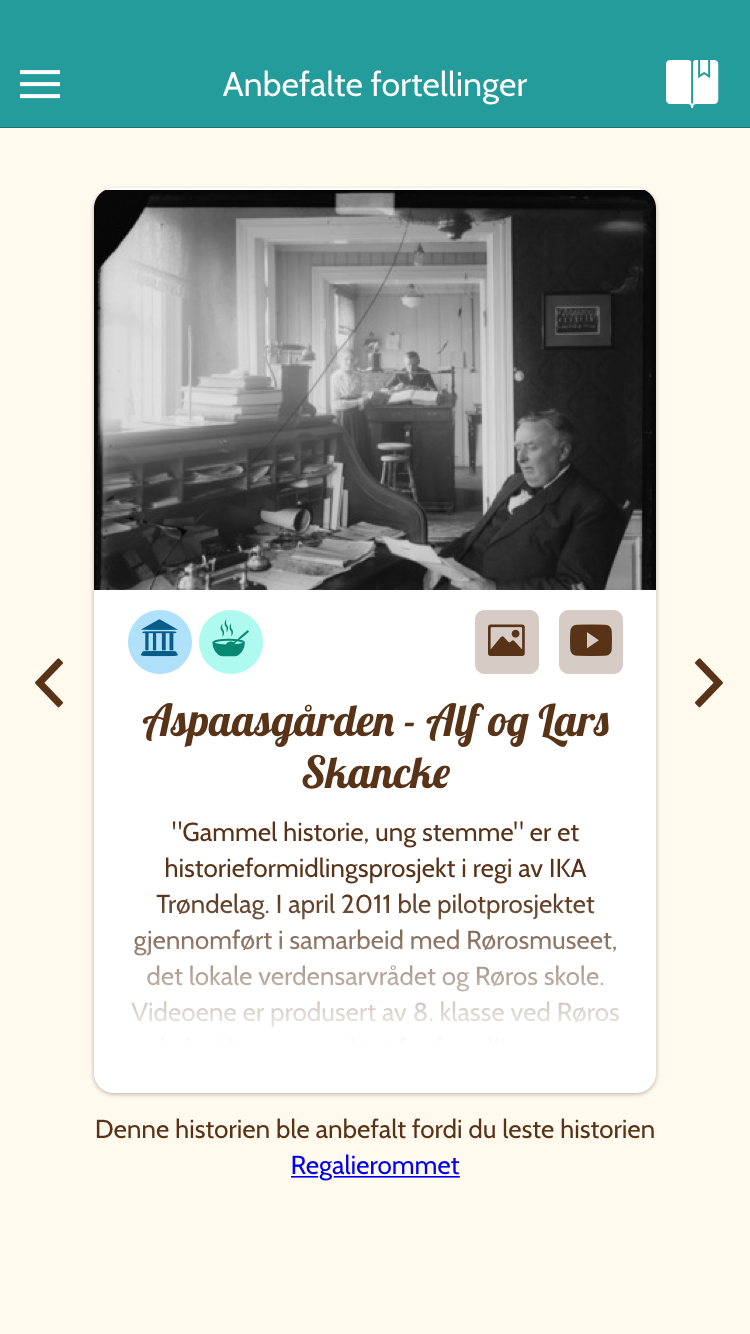
\includegraphics[width=0.4\textwidth]{fig/screenshot_recommendations}
		\caption{Recommendation view}
		\label{Fig:recommendation_view}
	\end{figure}
	
	\item[Story view] \hfill \\
	This view displays the chosen story in detail. There is a box which displays the media files associated with the story. The tabs above it will depend on which media types the story contains. Videos will be displayed by default if there are any, as they can be a major component of the story which should not be hidden in another tab. When tapping on a video or image it will be displayed in fullscreen mode. The user can give feedback on the story either by tapping the stars on the bottom part of the view, or by tapping the star icon in the top bar which will open up a modal. The modal will ask the user to rate the story, and the user can exit it by tapping “Ferdig” or by tapping outside of the modal. Tapping the bookmark icon will make the same modal as in the recommendation view appear. 

\end{description}

\begin{figure}[h!]
	\ContinuedFloat
	\centering
	
\includegraphics[width=0.4\textwidth]{fig/screenshot_story}
	\caption{Story view}
	\label{Fig:story_view}
\end{figure}

\section{Front-end - back-end communication}
\label{subsec:frontend-backend_communication}

Communication between front-end and back-end was handled using HTTP post requests.
AngularJS \$http is a core service for reading data from remote servers, which is called every time the application needs to add, retrieve, update or delete data. When an HTTP request is made, four fields are set: method, headers, URL and data. The method field determines the HTTP request method, which in this application is set to post, and the headers field sets the content type to JSON. The URL is the location of the remote server script that handles HTTP requests. In the data field the action to be executed is specified, in addition to any data needed to perform the desired action.\newline

Each HTTP request is managed by the same back-end PHP script. This script decodes the HTTP request, determines which action to perform and executes it. When the script has finished executing, a JSON response is returned to front-end with the desired data. "Get story" is an example of a request. When a user wishes to read a story front-end sends the JSON formatted paramaters userId, storyId and request type, in addition to the previously mentioned fields, as an HTTP request to back-end. Back-end retrieves story information from the database and Digitalt fortalt, which is then returned as a JSON formatted response to front-end. Other request examples are "Add user", "Edit user" and "Get recommended stories".

\section{Back-end overview}
The back-end design is divided into five sections, such that each section addresses a separate concern. A concern is a set of information that affects the code of the application. The value of such a separation is that it simplifies the development and maintenance of the application code. By splitting the code into separate parts the system is more logically structured, and cleaner code is achieved. The result is as an example that SQL related code is maintained by one part of the system, while HTTP processing is executed by another. Below is a description of the different back-end sections.

\begin{description}
	\item[Models] \hfill \\
	Consisting of the classes storyModel, userModel and preferenceValue. The models are used to temporarily hold information about a story, a user and a user's preference value for a story to be utilized by other files. Information is either retrieved from the database, sent from front-end, harvested from Digitalt museum's API or a combination of these. These models also contain formatting methods, which makes it possible to return story or user information to front-end.
	
	\item[Database] \hfill \\
	This section contains the classes dbStory, dbUser, dbHelper and harvesting. The db classes are responsible for accessing the database. dbStory contains methods for adding or retrieving story related information from the database and dbUser is responsible for user related information. dbHelper consists of more general methods and is the class which establish a connection with the database. The harvesting script is responsible for collecting all database stories from Digitalt museums API and adding stories to or updating stories in the database (see \textbf{Section \ref{sec:harvesting}}).
	
	\item[Personalization] \hfill \\
	Consisting of the classes computePreferences and runRecommender. This section computes preference values for each Digitalt fortalt story in the database for each user. runRecommender is also responsible for initializing the Mahout recommendation engine when a user's preference values have been calculated.
	
	\item[Recommender] \hfill \\
	This section consists of the Java code and recommender.jar file which make up the Mahout recommender (see \textbf{Section \ref{sec:personalization_how}}).
	
	\item[Requests] \hfill \\
	Contains the controller script, which receives and handles front-end HTTP requests and returns JSON responses (see \textbf{Section \ref{subsec:frontend-backend_communication}}).
	
\end{description}

\textbf{Figure \ref{Fig:overall_backend}} depicts the different back-end classes introduced in the previous paragraphs and give an overview of their dependencies.

\begin{figure}[h!]
	\centering
	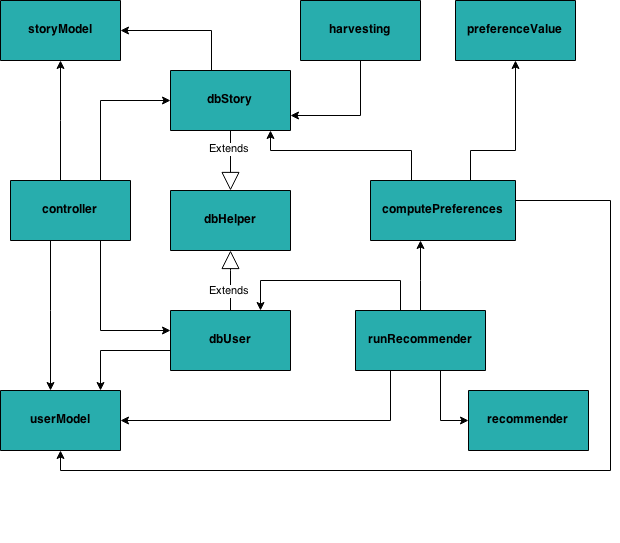
\includegraphics[keepaspectratio=true,scale=0.6]{fig/overall_backend}
	\caption{Class diagram of the overall back-end structure}
	\label{Fig:overall_backend}
\end{figure}

\section{Category mapping} 
\label{sec:categorymapping}

There are 31 subcategories presented at Digitalt fortalt. Each story can have 0 to 31 subcategories attached to it. To achieve content-based filtering the user has to select some categories of interest. To make it easier for the user, these subcategories are divided into nine main interest categories. Some of these categories were already predefined in a TAG CLOUD document provided by the customer, while the rest was changed according to discussions with the customer. The subcategories were put into the category interest field that fit them best, with some subcategories being in several category interests. In \textbf{Table \ref{Tab:categorymapping}} this mapping is illustrated. It is obvious that some category interests will have more stories, and some subcategories such as history contain more stories than most others. In such a way, it was intended to create nine category interests that contain roughly the same amount of stories. Even distribution of stories into category interests was intended, however, when a subset of stories was chosen this intention did not hold true as can be seen in chapter \textbf{Section \ref{sec:harvesting}}. Furthermore, the category interests needed to be distinct while still encompassing all the subcategories. 

\begin{table}[!h]
	\begin{center}
		\caption{Category mapping performed to facilitate, and simplify content-based filtering. Each subcategory is assigned to one or more category interests.}
		\label{Tab:categorymapping}
		\begin{tabular}{ | p{5cm} | p{12cm}|}
			\hline
			\textbf{Archeology} & Arkeologi og forminne \\ \hline
			\textbf{Architecture} & Arkitektur \\ \hline
			\textbf{Art and design} & Bildekunst, dans, design og formgjeving, film, fotografi, media, teater \\ \hline
			\textbf{History} & Historie, historie og geografi, kulturminne, sjøfart og kystkultur, språkhistorie \\ \hline
			\textbf{Local traditions and food} & Bunader og folkedrakter, dans, fiske og fiskeindustri, fleirkultur og minoritetar, Hordaland, kultur og samfunn, kulturminne, musikk, Rallarvegen, samer, sjøfart og kystkultur, språk, tradisjons- mat og drikke \\ \hline
			\textbf{Literature } & Litteratur, teikneseriar \\ \hline
			\textbf{Music} & Musikk \\ \hline
			\textbf{Nature and adventure} & Fiske og fiskeindustri, naturhistorie, sport og friluftsliv \\ \hline
			\textbf{Science and technology} & Fiske og fiskeindustri, fotografi, "kjøretøy, bil og motor, veitransport", media, "natur, teknikk og næring", "teknikk, industri og bergverk", skip- og båtbygging \\ \hline
		\end{tabular}
	\end{center}
\end{table}


\section{Digitalt museum's API and harvesting}
\label{sec:harvesting}

All content related to stories displayed in the application was collected from Digitalt fortalt. At the request of the customer the stories collected are limited to the areas Nord-Trøndelag and Sør-Trøndelag. The reason for this was that it would increase the likelihood of users reading similar stories, and thus make it easier to evaluate the personalization. The API \cite{digitaltMuseum} used to retrieve stories belongs to Digitalt museum. This API enables search through data from Digitalt museum, displaying pictures, and provides access to an XML representation of available objects. Digitalt fortalt is established on the same technical platform as Digitalt museum \cite{HM2}. This makes the integration better between the two and the remaining services in Norvegiana. Norvegiana is a data model, database and a web service with the purpose of making cultural heritage information more accessible \cite{HM3}. Example services available in Norvegiana are Digitalt museum, Digitalt fortalt, Arkivportalen and Musikkarkiv.\newline 

Some info, such as the categories for each story, are harvested and stored in the database. This is mainly to facilitate personalization. The actual story and the related media are fetched from Digitalt fortalt at the request of a specific story from front-end. At the time of writing the number of harvested stories is 169. This may vary as the harvesting is done each day. The stories are distributed unevenly over the nine categories; both the history and local traditions categories have over one hundred stories connected to them, while the literature category only have two stories connected to it. Media formats distribution also varies, with only fifteen stories having sound and both picture and video included in over one hundred stories.  

\section{Personalization}
\label{sec:personalization_how}

Users receive recommended stories by means of content-based and collaborative filtering, described in \textbf{Section \ref{sec:personalization_algorithms}}. The system gathers information about the stories and the users, and feeds this information into the recommender engine Mahout which produces a list of recommendations for the specified user. The details of Mahouts inner workings will not be presented here. What will be described is how the input data delivered to Mahout is gathered and produced by our application, what methods of Mahout is used and when they are used, and how the resulting list of recommendations is dealt with.\newline

Both content-based and collaborative filtering rely on giving a numerical value that express how much a user likes a story. We call this a preference value. In our application this value is computed by combining several measures representing different types of user feedback. These are: the rating a user have given to a story, the categories the user has expressed an interest in, the number of times a story has been recommended to the user, the number of times the story has been opened and the number of times a story has been put in the to-be-read list. Weights are assigned to the measures to differentiate between what impact they should have on the preference value. Rating is considered the most important user feedback, since this value is given to a story by direct user action. The other measures are either less connected to a specific story or more intangible. When computing recommendations, preference values for all stories for the user in question are calculated first.\newline

Each time Mahout is run, up to ten recommendations are inserted in the database. How these are chosen depends on a number of factors. Since a requirement from the customer was to include false recommendations, one of the recommendations is always picked from the lower parts of the recommendation rankings. The other stories are picked from the top of the rankings. Depending on two factors some top recommendations may be skipped for a given run. The first of these factors is that rated stories are not recommended again to the user (only an issue for content-based filtering). The other one is whether the list of recommendations should be added to the existing list of recommendations browsed by the user in the recommendation view or not. When adding to the existing list, recommendations should not be repeated.\newline

Mahout uses a data model and a similarity model to compute recommendations. The data model is a collection of triplets, where each triplet consists of a user ID, a story ID and a preference value. The selection of which preference values to include is different in content-based and collaborative filtering. The similarity model is also different for content-based and collaborative filtering. A description of these differences follows in the subsequent sections.    

\subsection{Content-based filtering}

When doing content-based filtering, the input data model consists of a collection of all the preference values for the user we are making recommendations for. This means that the size of the model will be equal to the number of stories harvested from Digitalt fortalt. To make recommendations Mahout also need measures describing how similar stories are. Similarities between stories are computed based on the subcategories found in the second column in \textbf{Table \ref{Tab:categorymapping}} using the cosine similarity formula: 

\begin{equation}
similarity = \frac{\vec{x}\cdot\vec{y}}{||\vec{x}||\cdot||\vec{y}||}
\end{equation}

The dot product in the numerator is in our system equivalent to the number of common subcategories for two stories, while the denominator is the product of the square roots of the number of subcategories for each of the two stories. If two stories have exactly the same subcategories the similarity value will be 1, and if they do not share any subcategory the value will be 0. \newline

These similarities are put in a CSV file at the time of harvesting. This file is read before the recommendations are computed and the similarity values are put in the appropriate Mahout objects. Mahout then uses the data model and the similarity model with similarity values for all possible pairs of stories to produce a ranked list of recommendations. This list is enhanced with an explanation of why a story was recommended, using a Mahout method that returns the stories most influential for a given recommendation.


\subsection{Collaborative filtering}

Collaborative filtering uses a data model with multiple users. Only the stories a user has rated will be included in the data model since this is the most precise user feedback. In our application collaborative filtering is done by combining two different methods provided by Mahout, namely item-based recommendation and user-based recommendation. The item-based approach creates a similarity model based on similarity between items in the data model using a logarithmic Likelihood function, while the user-based approach creates a similarity model based on similarity between users in the data model using Pearson correlation. To prevent dissimilar users from affecting the recommendations in the user-based approach, a threshold value for the similarity is set. The two lists of recommendations are produced and then merged, assuming both have content to get one list of ranked recommendations. If only one of the lists has content then the predicted rating for the story is used to decide what story to serve next.\newline

As was noted in \textbf{Section \ref{sec:personalization_algorithms}} collaborative filtering requires a large amount of data to make recommendations. Since only rated stories are included, collaborative filtering cannot be run when a new user starts using the application as the user will not be part of the data model. The criteria for using collaborative filtering needed to be met is that the user has rated at least ten stories which at least ten other users also have rated. In the event of too few collaborative story recommendations content-based filtering is used. 

\section{Database design}
\label{sec:database_design}

The database was designed with the goal of facilitating the recommendation of stories to users. The data model underpinning the database is visualized in the ER-diagram in \textbf{Figure \ref{Fig:er_diagram}}. User and story are the central entities in this diagram, since the goal of the application is to connect users to stories. Both of these entities has a number of attributes describing the entity. The central relationship in the diagram is the recommendation-relationship, where a user and a story is connected. This connection is described by some additional attributes, such as rating, tag and state. \newline

To make the right connections between user and story, some attributes describing the user and the stories are necessary to store in the database. For instance, in order to make recommendations based on nine predefined categories, every story is mapped from subcategories gathered from Digitalt fortalt to one or more of the nine categories (see \textbf{Section \ref{sec:categorymapping}}). A user is connected to one or more of these categories by the setting of personal preferences. In addition, the database stores information about the changing state of recommended stories in order to make better recommendations. \newline

Another goal of this project was to provide some research data to the customer. To do this, some data about the use of the application is stored. This includes registering what actions are taken during a user session. The state entity records changes in the state of stories connected to a user. For research purposes the customer also wished to know the relationship between satisfaction of a story (i.e. the rating) and the media format contained in the story.

\begin{figure}[h!]
	\centering
	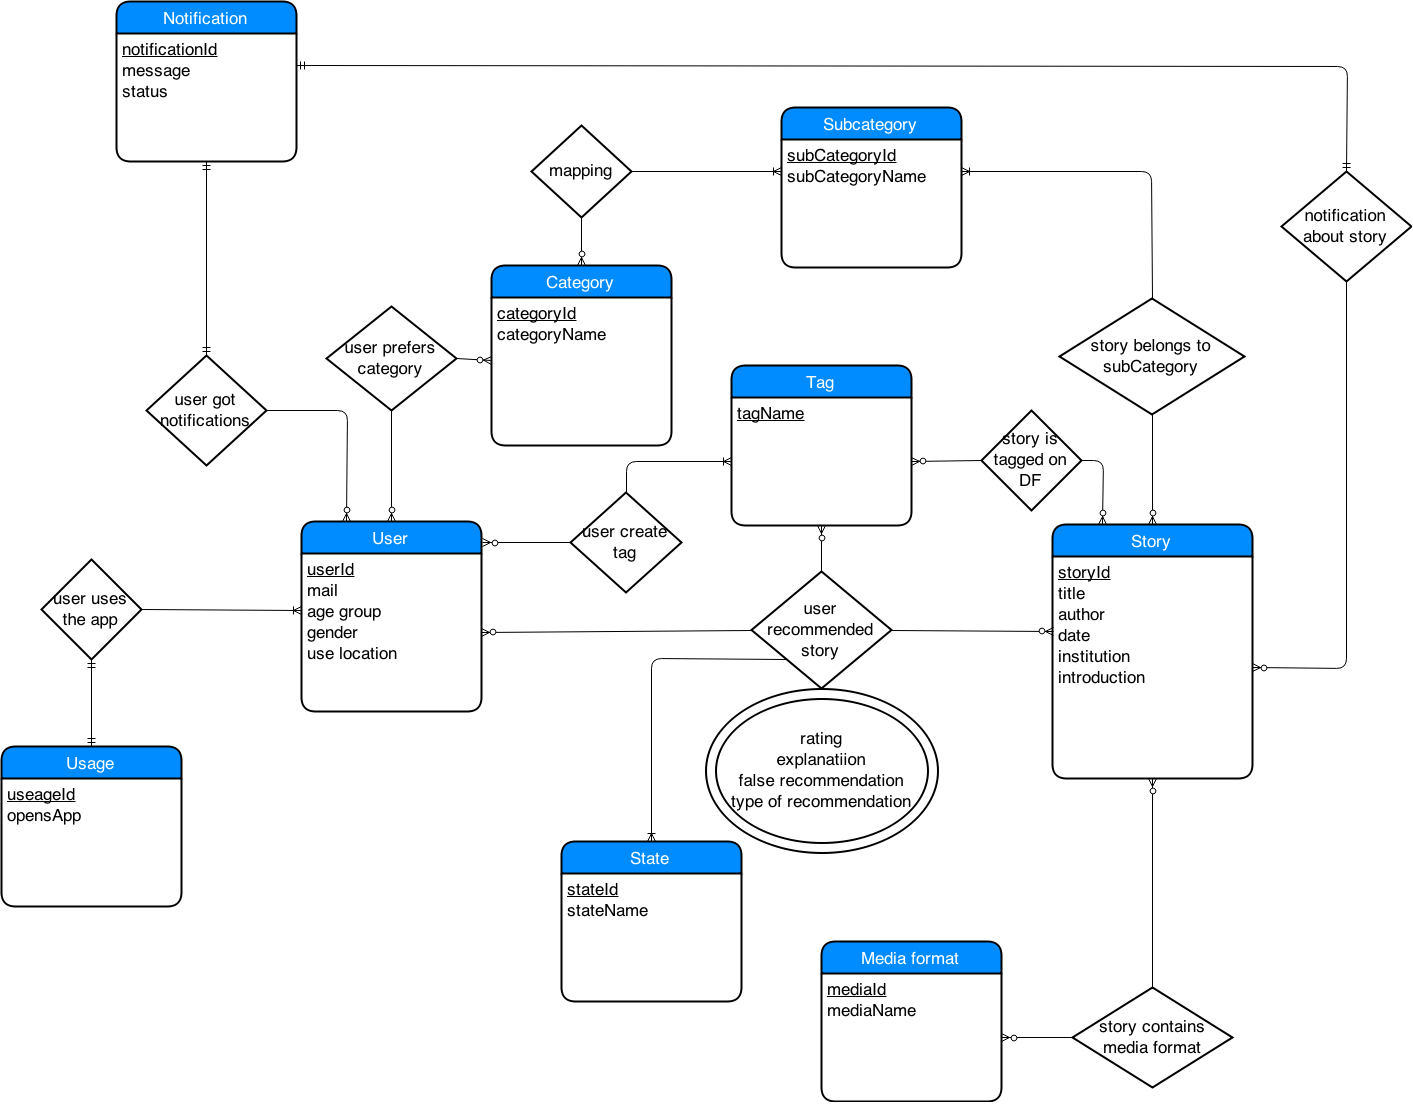
\includegraphics[width=\textwidth]{fig/er_diagram}
	\caption{ER-diagram showing the data model.}
	\label{Fig:er_diagram}
\end{figure}


\section{Docker}
\label{subsec:docker}

Docker \cite{EHW2} was made to help automation of application deployment. This happens by providing a virtual operating-system-level abstraction. This means that on a server, it is possible to run several virtual operating systems called docker images, which can easily be deployed to another server. This is beneficial for software development, because it means it is easy to setup identical back-ends at different locations. The customer used this on their servers, which made using it during development a good choice as well. A benefit of using docker is that it can directly access repositories on Git. This means that the latest revision is guaranteed to run when starting the back-end. However, there are also drawbacks. It is not easy to update files within the docker image currently running without rebuilding it. This means that to update a single line of code, the whole image needs to be rebuilt. Which means that while the newest revision is guaranteed to be running, any changes made to the application after the start of that docker image requires manually stopping, rebuilding, and restarting the docker image. \\

A docker image based on Ubuntu was used. In the Dockerfile, which is used to automate the deployment, all required dependencies were installed through Ubuntu's command line. A Linux, Apache, MySQL, and PHP (LAMP) stack, Java, and Mahout were the most critical dependencies. The setup of these tools was written to files which are downloaded from GitHub at runtime along with the back-end source files. After the Dockerfile is run an image is built and launched as wanted.


\cleardoublepage
%===================================== CHAPTER 8 Implementation =================================

\chapter{Implementation}

This chapter discusses the details of the system implementation process, both for front-end and back-end implementation, but also how the project was managed throughout the process.


\section{Project progression}
The project progression derives from the product backlog (\textbf{Appendix \ref{app:product_backlog}}), meeting minutes (\textbf{Appendix \ref{app:meetingreport}}) and Trello archive and will only briefly summarize what was done at each sprint and only serves as a "quick tour" through the development process.

\begin{description}
	
	\item[Sprint 1 - 23.01.15 - 30.01.15] \hfill \\ 
	The first week mainly consisted of getting familiar with each other and the assignment. As soon as the introductions were done, we talked about our personal goals to set the expectation as a group. We formalized the rules of engagement (\textbf{Appendix \ref{app:rules_of_engagement}}) for the group to sign, and also delegated responsibilities. Later we established a meeting agenda with the customer and met with them for the first time.
	
	\item[Sprint 2 - 30.01.15 - 06.02.15] \hfill \\ 
	In sprint 2 we began planning and formalizing the requirements. Large sections of work like sketching a WBS (\textbf{Figure \ref{Fig:wbs}}), generating a product backlog (\textbf{Appendix \ref{app:product_backlog}}), and making use cases were done this week. Other design work like the architecture and UI mock-ups were also started on.
	
	\item[Sprint 3 - 06.02.15 - 13.02.15] \hfill \\ 
	This was the first week of development. We started testing the API (\textbf{Subsection \ref{subsec:back_end_tools}}) and finalized some paper prototypes for user testing (\textbf{Subsection \ref{subsec:prototype}}) and also completed the design for the database and overall system architecture (\textbf{Figure \ref{Fig:architecture}} and \textbf{Figure \ref{Fig:er_diagram}}). Research on personalization (\textbf{Section \ref{sec:personalization_algorithms}}), the front-end framework Ionic (\textbf{Section \ref{subsec:ionic}}), and differences between the two operating systems \todo{ref crossplatform OS}IOS and Android were noted.
	
	\item[Sprint 4 - 13.02.15 - 20.02.15] \hfill \\ 
	For this sprint we analyzed the existing work done in the past (\textbf {Section \ref{subsec:stedr}}) to see if would fit our needs, and continued the research on collaborative filtering (\textbf {Section \ref{sec:personalization_algorithms}}). Some group members also spent time learning Docker (\textbf {Subsection \ref{subsec:docker}}). We mapped the Digitalt fortalt categories to our own (\textbf{Section \ref{sec:categorymapping}}) and conducted and evaluated the paper prototype tests as well. During this sprint the database code was also starting to take shape. We did a prioritization of the functional requirements in order to better plan the next sprint.  
	
	\item[Sprint 5 - 20.02.15 - 27.02.15] \hfill \\ 
	In this sprint we managed to get the harvesting (\textbf {Section \ref{sec:harvesting}}) up and running after the database was ready. A lot of work with the internal models on the back-end was done. The front-end team moved steadily though the initial work on the prioritized views (login, story and list). There was also a revision of the prototype to accommodate the customer's feedback from their user tests.
		
	\item[Sprint 6 - 27.02.15 - 06.03.15] \hfill \\ 
	Finalizing the database communication was done in order to fully test the front-end and to get the back-end team started on the personalization. The test plan (\textbf {Section \ref*{chap:testing}}) was in the stage of being attuned and formalized for the documentation. After the new prototype was finished, another round of user tests were conducted and the work continued on each of the application views.
	
	\item[Sprint 7 - 06.03.15 - 13.03.15] \hfill \\ 
	Some work to meet a report delivery was done early in the sprint. Later in the sprint, the back-end was showing good progress on finding/testing a suitable filtering framework, while the front-end refined the appearance of each view to better fit the user needs. The was also work done on resolving some issues with the server communication.
	
	\item[Sprint 8 - 13.03.15 - 20.03.15] \hfill \\ 
	The application was taking shape on many fronts, so this week we worked more on video support and started with the on-boarding section of the application. On the back-end the Mahout (\textbf {Section \ref{sec:personalization_how}}) framework setup was on the way. There was also some work spent on testing.

	\item[Sprint 9 - 20.03.15 - 27.03.15] \hfill \\ 
	This week we polished some features and functionality to hit the milestone Beta version (\textbf {Section \ref{sec:milestone_plan}}) in order to prepare the application for some testing in the wild during the upcoming Easter. Further development on the Mahout framework, content-based filtering and fixing of some unforeseen issues on the harvester was also done.
	
	\item[Easter - 27.03.15 - 07.04.15] \hfill \\ 
	The application was tested under informal conditions on family and friends, a so-called "in the wild" test.
	
	\item[Sprint 10 - 08.04.15 - 17.04.15] \hfill \\ 
	We dealt with the feedback from usability tests conducted during the Easter. Some platform-specific issues needed some focus to be resolved. We did some more polish on the views and cleared out some front-end bugs. on the back-end, work continued on filtering both collaborative and content-based, which it would for the rest of the sprints. 

	\item[Sprint 11 - 17.04.15 - 24.04.15] \hfill \\ 
	The application is beginning to be nearly finished on a functional level. Resources were dedicated to polishing, and bug fixing became the focus while a lot of testing was conducted on the server. The last big task that the back-end worked on was to finalize the filtering.

	\item[Sprint 12 - 24.04.15 - 01.05.15] \hfill \\ 
	Sprint 12 was similar to sprint 11, but there was a significant increase in the workload this week due to the upcoming final milestone of having an application ready for delivery to the customer. We intended to accomplish this by the end of this week. This did not happen, but we had aimed for a final build earlier than necessary. We planned for some last minute changes and allowed time to fix undiscovered bugs, which was exactly what happened. We also used some extra time for unit and system testing.
	
	\item[Sprint 13 - 01.05.15 - 08.05.15] \hfill \\ 
	This week was spent on various bug fixing for some members for the group, while the majority did mainly report and documentation work. We planned an acceptance test with the customer the following week. We went through the application and did extensive functional testing prior to the customer meeting.

	\item[Sprint 14 - 08.05.15 - 15.05.15] \hfill \\ 
	During the testing done the week before, more undiscovered issues were uncovered and we needed some more time for polishing and fixing. We had not yet locked in a date for the customer to do an acceptance test, except before the end of the month. The customer agreed to set up a final meeting the following Monday, which we felt would give us time to take care of our main issues, and even give us some time to go the extra mile.
	
	\item[Past 15.05.15] \hfill \\ 
	At the start of the week we met with the customer to go through the functionality in conjunction with the functional requirements to see if the customer also thought we hit our goal (See \textbf {Section \ref{sec:acceptance_test}}).\newline
	  
	Work was conducted after the last sprint(sprint 14) this was mainly fixing some bugs, finalizing the report and the application and source code handover. The final burn down of the work progression for all the sprints is shown below in \textbf {Figure \ref{Fig:burnDownAfter}}.
	
\end{description}

\begin{figure}[h!]
	\centering
	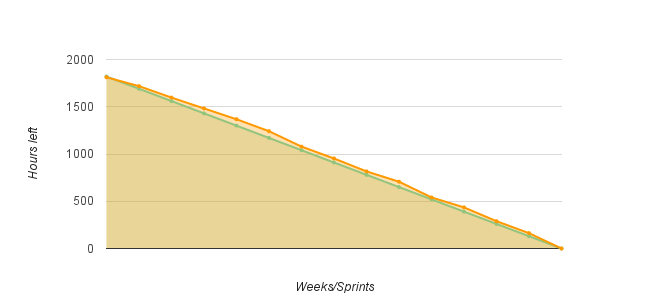
\includegraphics[width=\textwidth]{fig/burnDownAfter}
	\caption{Final burn down chart}
	\label{Fig:burnDownAfter}
\end{figure}

\section{Front-end}

This section will be an elaboration of some challenges and limitations that arose during the creation of the user interface, both concerning the design and the implementation aspects of the process.

\subsection{Designing the user interface}
\label{subsec:prototype}
The user interface design was an essential part of the project, as the customer prioritized usability over all other non-functional requirements. The design therefore went through many iterations of working on a prototype and continually getting feedback from customer and user tests. This feedback loop was important as the customer did not have all the specific requirements to the application from the beginning, and because making everything easy to understand for the user was also challenging. Balsamiq was first used to create a basic wireframe, but as its functionality was limited, the next iteration of the design was made using Proto.io. This made it possible to receive better feedback on the flow of the app and not just the views individually. \newline

While designing the user interface, some attention was paid to the projects described in \textbf{Section \ref{sec:existing_solutions}}. The group analyzed this previous work as a basis to decide what would be good or bad design choices for "Vettu hva?". A few general conclusions described in \textbf{Section \ref{sec:existing_solutions}} were that having static images occupying screen space is poor design, and that lists are normally easier to navigate than maps.\newline


The target audience for the application included both those who have an interest in cultural activities, and also those who do not have any interest or experience about this, so as to encourage more of the general population to discover an interest in the subject. A specific target audience of 16-19 year old teenagers were promoted as a possible focus, because of the possibility of encouraging a young audience to develop an interest in cultural heritage. However, this was not stated until around  midway in the project timeline. This fact made it difficult to consider target audience when making design decisions. \newline

The prototype has been through multiple iterations. Early on, it was imagined to have a sort of “magic” discovery function where a user would for example rub a crystal ball and receive a recommended story. This idea was later discarded because the team and customer realized
 it would be better usability to present the user with multiple recommended stories that they could simply browse through instead.\newline

Another of the early ideas was for the user to receive a “daily story” or some sort of schedule for being presented with recommended stories. However, due to workload and time constraints, this requirement was heavily down-prioritized. The most important parts were the personalization and usability aspects, so receiving notifications seemed like an unnecessary extra feature.\newline

In the first prototype a media preference view was also included when creating a new user. In this view the user should put the media formats (text, images, video, audio) in order by which format the user preferred. This was discarded in the second prototype, as it was difficult for users to understand the purpose of it and the customer agreed it was not necessary. 
\begin{figure}[h]
	\centering
	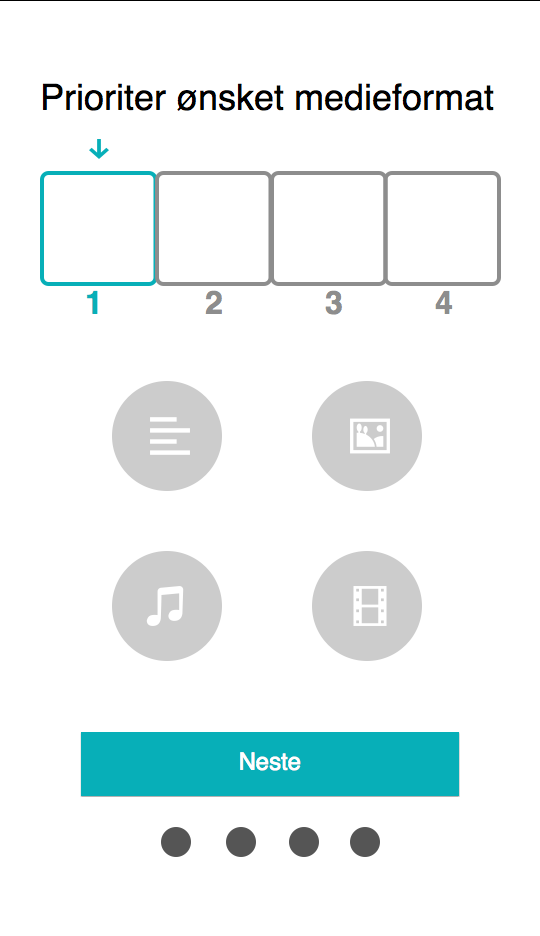
\includegraphics[scale=0.5]{fig/prototype_media}
	\caption{Media preference view from the first prototype which was later discarded.}	
\end{figure}

The application uses many different icons in various parts of the interface, and these have been the source of much debate and redesign. The icons used to represent categories were not always understood by users, and some categories like “local tradition and food” were difficult to represent universally with just a single icon. Also the bookmark icon shown in the upper right area of \textbf{Figure \ref{Fig:prototype}} was confusing to some users, and there was a concern in the team that this icon might not accurately represent that it allows the user to save the story in a bookmark list.\newline

A big issue for the interface design has been the handling of the different media elements (text, pictures, audio, video) and how these should be positioned relative to each other. For a while the team designed the application to have one tab for each of these four elements in the story view, as shown to the left in \textbf{Figure \ref{Fig:prototype}}. The customer had a concern that this might not be the optimal solution, as a user would for example not be able to read text and view pictures simultaneously. After some discussion, the interface was redesigned so that the text would be persistent, and instead the user could tab between pictures, audio, and video. The resulting design can be seen to the right in \textbf{Figure \ref{Fig:prototype}}. \newline

\begin{figure}
	\centering
	\begin{subfigure}[h]{0.3\textwidth}
		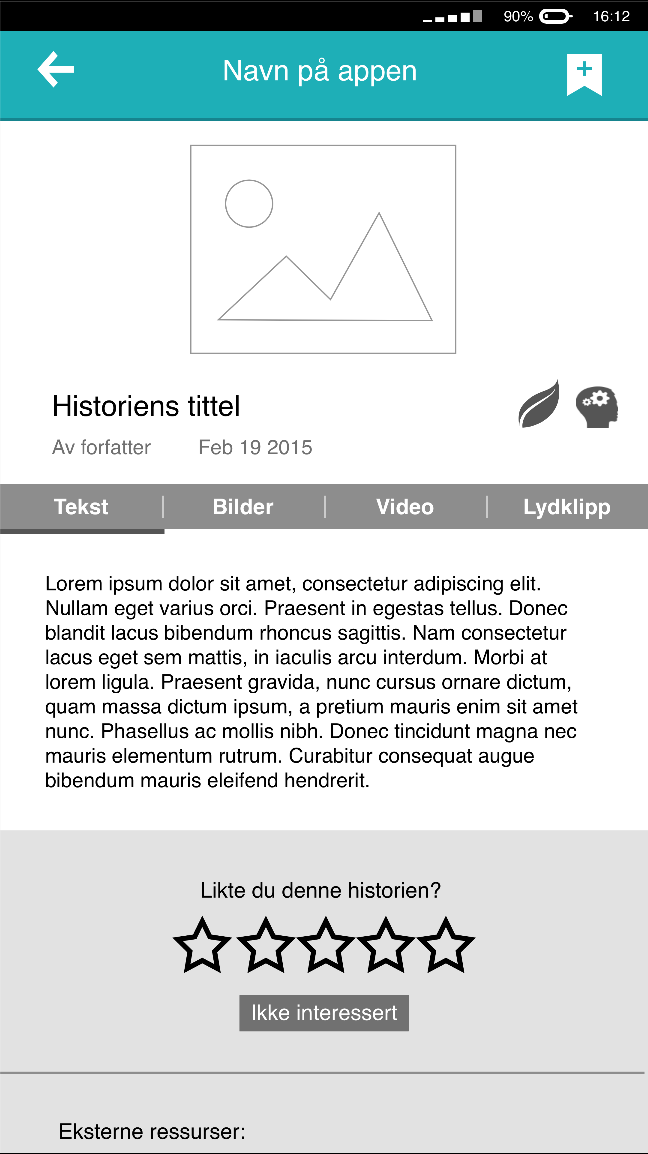
\includegraphics[width=\textwidth]{fig/prototype1}
	\end{subfigure}
	\begin{subfigure}[h]{0.3\textwidth}
		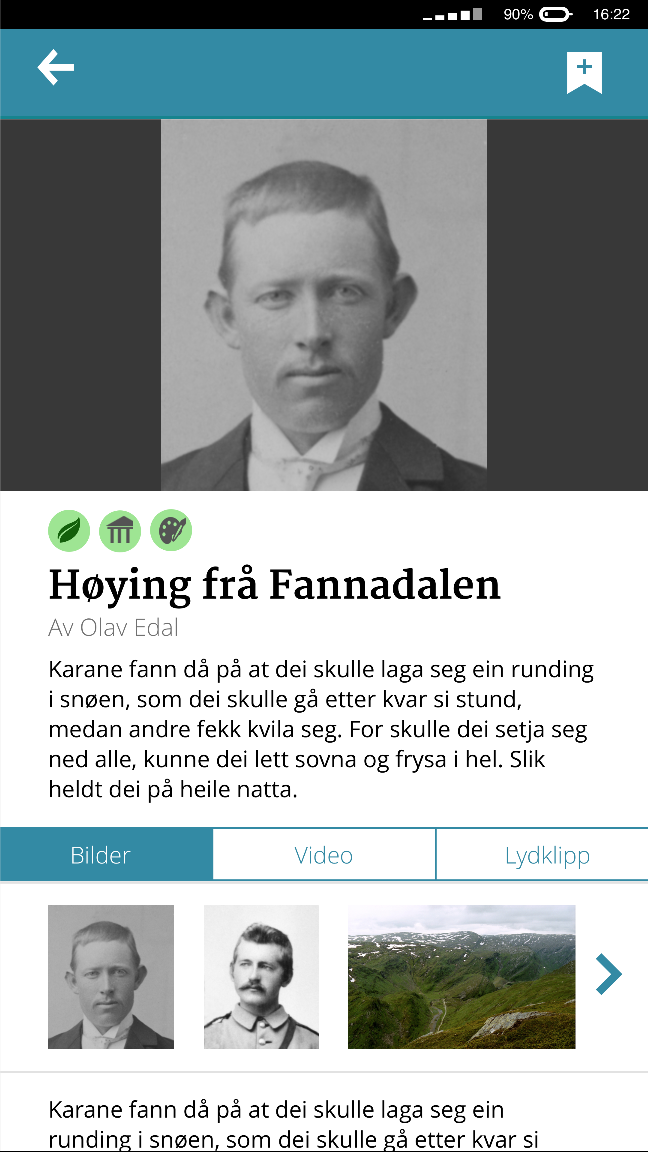
\includegraphics[width=\textwidth]{fig/prototype2}
	\end{subfigure}
	\begin{subfigure}[h]{0.3\textwidth}
		
\includegraphics[width=\textwidth]{fig/screenshot_story}
	\end{subfigure}
	\caption{Comparison of the story view in the first and second versions of the prototype and the final design implemented.}
	\label{Fig:prototype}
\end{figure}


\subsection{Implementing the user interface}
\label{subsec:user_interface}

Early on in development, the team discovered several limitations to the Ionic framework. For example, when using a list to display stories, it was not possible to swipe the list both left and right. The idea was to swipe one way to add a story to be read later, and swipe the other way to reject a story from the list entirely.  Because this proved to be impossible, the views were redesigned into a different solution which was much less based around swiping.\newline

As this is an application for mobile devices, it had to be adapted to work on different screen sizes. The team found that it would most likely be best to target a relatively small screen size and then simply enlarge it for bigger screens. This eliminated the issue of having to compress the components to fit smaller screen sizes and potentially be forced to redesign the whole view to fit small screens.\newline


Adopting accurate naming conventions for the different components has also been a considerable issue. Stories can be saved in bookmark lists, but these lists have interchangeably been called collections and tags in the system. Also when asking a user to input their preferred categories to receive stories from, there has been some confusion because of interchangeably calling these categories for interests,  preferences, and categories.\newline

Implementing media, and especially video, has been a challenge in the project. An issue with this has been that playing videos is handled differently on iOS and Android, which had resulted in some bugs that only appear on one platform and not the other. These types of issues have been problematic to fix and has taken up much time. In addition, the videos provided by the Digitalt fortalt website come from different sources. Some of them are Youtube videos, others are Vimeo videos, and there are also other variations. Integrating all these different formats smoothly into the application has been a considerable challenge as well. \newline

Being able to reject a recommended story was a feature that was supposed to be implemented, but it was more difficult than it seemed. The problem was with the slide component from the Ionic framework, which did not do well with dynamic content. When removing a slide from the middle of the list of recommendations, it would not update properly and swiping did no longer work. \newline

It was also decided to remove the "not interested" option when rating a story. This was considered when testing the prototype, but was not decided until after the development had started. It was not intuitive what the button would actually do, and the user can convey the same "not interested" message in other ways. In order to rate, the user has to at least look at the story. If the user does not like the story after looking at it, then it is both more intuitive and useful that the user gives a low rating rather than "not interested". 





\section{Back-end}

This section describes the development of each part of the back-end. It aims to give a timeline of the development and explain how and why important decisions were made. The different parts described here are Docker, the database, the personalization, the choice of language and the e-mail part of the application.  

\subsection{Docker}

Using Docker as a deployment tool proved easier than initially expected. This is mainly because there exists a good amount of documentation and examples online. Initially the Docker setup was based entirely on a project called tutum \cite{EHW3}. Using this projects Dockerfile it is possible to only specify the Git repository of an application to have an Apache server running with this application. Furthermore, it is possible to define a password to use for the database. This suited the back-end work very well since it filled the initial requirements. However, as requirements developed and understanding of Docker increased, a more tailored and advanced setup was used. In this setup a second image is used to save the database between restarts, which means that it is possible to update code without having to start the database anew. In addition to this, harvesting from Digitalt fortalt is performed at 03:05 server time, each night. \\

Once work on personalization started it was necessary to have Java in the Docker image as well. This proved uncomplicated and worked as intended. Passwords and other important keys were put in a separate file that can be included along with the Dockerfile where this is required.

\subsection{Database}

Based on the first version of the functional requirements for the application, an initial ER-diagram was made in the middle of February. At this stage the customer and the team had not come to an agreement on a prioritization of the non-functional requirements. This meant that it was for instance not clear how important the performance of the system would be for the customer, an attribute of the system which would influence how much info should be stored for each story in the database versus how much info should be retrieved from Digitalt fortalt every time a user views a story. However, the changes to the initial diagram have been relatively minor. Some of the alterations were based on updated requirements from the customer (for instance regarding research data), while others stemmed from the group and were optimization of the data model or changes made to facilitate the personalization.\newline

The relational database was created from the ER-diagram using the mapping algorithm in \cite[p.270-278]{AS2}. Some of the tables in the database has the potential for NULL values, but this was accepted as it was considered more important to keep the mapping from one entity to one table. In addition, the database already had quite a few tables and further splitting would make the extraction of information more costly, with numerous join operations. \newline 

The team did not understand how to do the personalization until mid March. The decision on how to do this introduced changes to existing tables and the need to create additional tables and views in the database. Mahout had requirements for the input data, which meant that a view was created to store all the necessary data for collaborative filtering. Using this view made it straightforward to put the desired data from the database into Mahouts data model.

\subsection{Personalization}

At the start of the project much time was devoted to understanding content-based and collaborative filtering and how the theoretical descriptions of these techniques could be turned into a practical implementation in our application. When the back-end part of the group had a better understanding on how this could be done, an important decision was whether to use open-source recommender engines or to implement the algorithms ourselves. After studying the math and complexity involved in writing our own implementation it became clear that the best solution would be to use existing recommender engines, even if this would require some adjustments to already written code. \newline

As the project was nearly halfway through when the decision to use an open-source recommender engine was made, the team did not find the time to do a thorough review of the many different alternatives. This increased the probability of choosing the wrong tool to work with and violated the stated preventive action in the risk list (see \textbf{Appendix \ref{app:risklist}}). However, the customer suggested three different recommender engines that might be worth looking into, one of which was Mahout (see \textbf{Section \ref{sec:rec_tools}} for a evaluation of the three different engines). In choosing a tool the customer had done some research on, the group found that the risk of making a wrong choice decreased somewhat. In addition, Mahout presented its features in a way that resembled the groups research on filtering algorithms and it was therefore reason to believe that getting started with Mahout would not require much additional research. Of particular importance was the fact that Mahout offered a short explanation on how to do content-based filtering using their recommender engine. Most such engines provided functionality for doing collaborative filtering, but it was not always clear how content-based filtering could be done.\newline

Mahouts website provided some guiding on how to build a recommender which made it possible to use the tool without thorough knowledge of how the different methods worked. Most of the work in the beginning of doing the personalization thus centered around how to gather and produce data in a format acceptable to Mahout and how to treat the output recommendations. Content-based filtering was implemented first, as this was the customer's wish and because the first recommendations presented to a user would always be content-based. Since Mahout does not provide methods for finding similarities between items based on their attributes, the group had to implement this. There exist a vast number of functions to compute similarity between objects. The group did some research on different similarity measures, but the literature did not provide a clear-cut answer to which measure was best fitted to our data. Cosine similarity was chosen for its simplicity and because a story's subcategories lent itself well to be represented as a vector.\newline

The customer requested the use of both item-based and user-based collaborative filtering. There was some doubt in the group as to whether the produced recommendations from the two methods could be combined, but it was found that this was possible as both take the same data model as input. When doing user-based collaborative filtering, a threshold value had to be set to tell the recommender engine which users should affect the recommendations. This concerns the similarity found between users. It was difficult to set this value as the computation of the similarity is done by Mahout and because the group did not know what threshold value would be reasonable to set. The value is set by means of trial and error, looking at the resulting recommendations produced using different values, and by looking at example use of this method. \newline

A challenge in the project has been to assess the quality of the recommendations. Reasons for this has been the limited amount of harvested stories and the use of Mahout as a black box. The first point was a limitation set by the customer. They wanted to limit the amount of harvested stories to ease the evaluation of "Vettu hva?". With fewer stories the probability of different users reading the same stories would increase, and thus require fewer users to get the collaborative filtering running (the cold start problem described in \textbf{Section \ref{subsec:prestudy_collaborative}} would be resolved faster). \newline

The second point was down to the implementation of the project and mainly concerns collaborative filtering. Content-based filtering has fewer variables and it was possible to check if input categories produce recommended stories that in fact are connected to those categories. Collaborative filtering involves more variables and it was not obvious from the raw data to see which users should influence recommendations for a user and what weights to assign to the different users preference values. In general, collaborative filtering finds patterns in the data that are less obvious found there than content-based filtering. By using Mahout as a black box this pattern finding has been hidden to the team. This could have been remedied by studying the implementation of Mahout, but the time required to do this was not found to be within the confines of the project. A broader test of the application with real users could also have given some insight into the quality of the recommendations, but this was outside the scope of the project. \newline


\subsection{Language}
\label{subsec:backend_language}
\textbf{PHP}\newline
PHP is a server-side scripting language produced by The PHP Group that is especially suited for web development  \cite{HM8}. It is a general-purpose scripting language often used to provide dynamic content from a web server to a client. During the pre-study period several reasons for choosing PHP as the main back-end language were presented. Firstly, all back-end team members were experienced in the use of PHP. Secondly, as inexperienced users of Docker, more documentation existed on how to implement PHP with Docker than with the other language alternatives considered. Lastly, it was easily combined with the HTTP protocol used by front-end to request and receive data (see \textbf{Section \ref{subsec:frontend-backend_communication}}).\newline

\noindent\textbf{Java}\newline
Java is a very popular general-purpose object oriented programming language developed by Sun Microsystems and later Oracle Corporation \cite{HM9}. Java was later in the project chosen as a secondary back-end language. This was because Mahout, which was used to implement the recommender engine (see \textbf{Section \ref{sec:personalization_how}}), is written in Java. 


\subsection{E-mail}

To create a user in “Vettu hva?” the user only needs to provide an e-mail address. E-mail was chosen as the identifier because it is unique for a specific person. When a user tries to log in and the e-mail does not exist in the database, a new user is created and the user is assigned a user ID and the ID is returned to front-end. A message is also sent to the provided e-mail, to confirm that the user is registered. If the e-mail already exists, the previously created user ID is returned to front-end and the user can continue where he/she left of. The mail service used to send the confirmation e-mail is an e-mail sending library for PHP called PHPMailer. Originally, the plan was to use the built in mail() function in PHP. However, in order for this to work a properly configured local SMTP server was required. This proved to be too much work for this assignment, so the solution was to use PHPMailer with a “Vettu hva?” gmail. PHPMailer can be used to send e-mails from existing mail servers, like Google Mail, by providing a username (gmail) and password.

\cleardoublepage
%===================================== CHAPTER 9 Testing =================================
\chapter{Testing}
\label{chap:testing}

The following subsections describes the strategies for the testing levels unit test, integration test, system test, costumer acceptance test and usability test. 
The unit, integration and system tests were done in a iterative manner. After the test suits were performed and the results were documented, the testers mended the issues in the system if they appeared during the test. After the mending, the test suit was executed again. This cycle was repeated until there was no issues left in the system and all test cases got the expected result. 
The issues that were discovered during all the tests are described in every testing level section. 


\section{Unit testing}
\label{sec:unit_testing}
The purpose of unit testing is to ensure that every piece of code that are implemented in the system are functional and correct. The group performed unit tests on new units of code before implementing them in the system. It was necessary to prioritize what units that should be tested, considering the amount of time given for the project. 
The units in this testing was PHP, Java and JavaScript classes. Therefore it was necessary to use different unit testing tools. Backend code was tested using PHPUnit framework \cite{KF2}, and JUnit \cite{jUnit} and the extension DbUnit \cite{dbUnit}. The user interface code was tested by using a AngularJS unit testing tool, called Karma \cite{KF3}. 
The classes that were tested is listed up under the unit column in \textbf{\Crefrange{Tab:phptesting}{Tab:karmatesting}}. The classes that were left out in the documented testing were tested manually by the developers. If issues were detected during the unit tests, the developers would mend the issues and run the tests again. This cycle was repeated until there was no issues left and all test cases got the expected result.

\subsection{Roles and Responsibilities}
To get a structured testing experience, the team had to delegate responsibility for the units. The roles correspond with the roles that were given at the start of this project (see \textbf{Section \ref{sec:scrum_team_and_roles}}), so the tester would have good knowledge to the code and know how it works. The delegated responsibilities is presented in \textbf{\Crefrange{Tab:phptesting}{Tab:karmatesting}}.



\begin{table}[H]
	\caption{Shows the delegated responsibilities in testing the back end part of the system written in PHP code.}
	\label{Tab:phptesting}
	\begin{center}
		\begin{tabular}{ | l | l | l |}
			\hline
			\multicolumn{3}{|c|}{\textbf{PHPUnit testing}} \\
			\hline
			\textbf{Unit ID} & \textbf{Unit} & \textbf{Responsible} \\ \hline
			U1 & Database Helper & Kjersti \\ \hline
			U2 & Database Story & Kjersti \\ \hline
			U3 & Database User & Eivind \\ \hline
			U4 & User Model & Eivind \\ \hline			
			U5 & Compute Preference Value & Kjersti \\ \hline			
		\end{tabular}
	\end{center}
\end{table}

\begin{table}[H]
		\caption{Shows the delegated responsibilities for the back end part of the system written in Java code.}
		\label{Tab:junittesting}
	\begin{center}
		\begin{tabular}{ | l | l | l |}
			\hline
			\multicolumn{3}{|c|}{\textbf{JUnit and DbUnit testing}} \\
			\hline
			\textbf{Unit ID} & \textbf{Unit} & \textbf{Responsible} \\ \hline
			U6 & Recommendation  & Audun \\ \hline
			U7 & Database connection with Java & Audun \\\hline			
		\end{tabular}
	\end{center}

\end{table}

\begin{table}[H]
	\caption{Shows the delegated responsibilities for testing the user interface.}
	\label{Tab:karmatesting}
	\begin{center}
		\begin{tabular}{ | l | l | l |}
			\hline
			\multicolumn{3}{|c|}{\textbf{AngularJS Karma testing}} \\
			\hline
			\textbf{Unit ID} & \textbf{Unit} & \textbf{Responsible} \\ \hline
			U8 & UI Login & Ragnhild \\ \hline
			U9 & UI Story View & Ragnhild \\ \hline
			U10 & UI Setting & Roar \\ \hline
		\end{tabular}
	\end{center}

\end{table}


\subsection{Test Cases}
The testers created test cases and used these as a guide for performing the tests. The test cases has an ID and describes exactly what the test should do, what input data to use and what is expected to happen when the test is running. The test cases are presented in \textbf{Appendix \ref{app:unittest}}.

\subsection{Detected and mended issues}
This section includes some of the most important issues that were discovered the unit testing, and how they were solved. 

In the database communication there was some changes done during the development which made it easier to handle the code. One example was to make the database connection return an array where the array keys matched the column names. This way made it easier to access the different values returned from the database.  
Another issue that was discovered with the media format per story that was not stored correctly in the database, because of an error during the harvesting of the stories from Digitalt Fortalt. These types of issues were solves with several checks to see if the information was in the right format or was not null. 

During the tests of the first version of the recommender it was running with the time of 11-12 seconds. This was improved by increasing the efficiency of the communication with the database. The recommender was more efficient when the insertion of preference values and recommendations was done with one insert statement to the database instead of respectively 167 and 10 statements. Previously the recommender fetched a whole table from the database with the preference values. Fetching preference values for a specific user instead of all users helped the recommendation module to run faster too.




\section{Integration test}
\label{sec:integration_testing}

Integration testing were performed after unit testing and before system testing. After the back end and front end code was testet and integrated, the integration testing started and focused on that these two modules communicated correctly and that the data was moving between them in the right manner. 
Because of the time limitations and the difficulty with learning a new interface to perform integration testing, the developers decided to perform the integration testing with unit test cases. The unit testing framework was already known to the developers and therefore easier and less time consuming to use. All the tests was executing by simulating HTTP requests from the UI and check that the back end gives the correct response to the specific HTTP request. 
If issues were detected during the integration tests, the developers would mend the issues and run the tests again. This cycle was repeated until there was no issues left and all test cases got the expected result. \newline


\subsection{Test cases}
The test cases were made by first having a closer look at the different modules and the data flows between them. The modules in question are shown in \textbf{Figure \ref{Fig:architecture}} of the architecture. for this project. The modules that the integration testing was performed on were front end(User Interface), back end with a general processing module and a personalization module, and the database. Because of the personalization module of our system is considered to be a crucial one, the most important data flows was the users input in the form of preferences and ratings. Also the communication with the database was crucial because the users information about ratings and preferences should be stored properly to get a beneficial recommendation. The test cases are described in \textbf{Table \ref{Tab:integrationtestcases}}.


\subsection{Detected and mended issues}

The following paragaph includes some of the most important issues that were discovered the integration testing, and how they were solved.

The issue that was considered to be the most time consuming one, was to update a user in the database. This issue was detected in the test case I.3. When a user was updated in the UI in the application, the unchanged information that should still be there, was deleted. This was tried to be fixed several times with methods that was not adequate. The problem was eventually solved with fetching all information about a user in the database, update the fields in the user model that had been changed, and then insert all the information in the database again. \newline

Other minor issues that were handled were syntax-issues, redundant code that created unnecessary confusion and missing table attributes in the database.\newline
Changes in the code where made to obtain better structure in the code, such as dividing long code files into smaller ones and to make sure functions returns a response if an error occur. \newline

Due to a misunderstanding between frontend and backend developers, the database returned names of category preference and story category, and not ids. \newline


\section{System testing}
The system testing were perfomed after the unit test and integration tests. The test gave the developers a measure of whether the system met all the goals set for the project.  The system test included performing a black box testing of the system, where the test cases was based on the use cases(\textbf{Section \ref{subsec:use_cases}}) and the specified requirements(\textbf{Section \ref{subsec:summary_functional_requirements}})  defined earlier in this report. \newline
In this test one of the developers were executing the test. Because it is a black box test, the tester executed the test cases with no access to the code. The tester went through all of the test cases one by one and performed the test cases manually. If issues were detected during the integration tests, the developers would mend the issues and the tests was runned again. This cycle was repeated until there was no issues left and all test cases got the expected result. Due to the time limits of this project the team were not able to write scripts to perform the test cases. \newline

When the system test was performed, the testers evaluated the tests results and then decided if the system as a whole fulfilled all goals for the project. If issues were detected, the developers would mend them and run the tests again. This cycle was repeated until the all the test cases got the expected result. The test should, if done in the expected manner, help the developers of this project to verify and validate if the application meets all the requirements.\newline

\subsection{Test cases}
The test cases cover the use cases in \textbf{\ref{subsec:use_cases}} and requirements in \textbf{\ref{app:functional_requirements}}. 
Each test case has a test identifier and an approach for the tester, and a description of what was intended to happen when the test case was performed. The tester will be referred to as “the user”. 
Some of the test cases have a dependability of other tests. If an issue is detected in one test case, it might cause issues in its dependent test cases. \textbf{Table \ref{Tab:systemtest1}} and \textbf{Table \ref{Tab_systemtest2}} are presenting two of the test cases that were used. The whole test case document are in \textbf{Appendix \ref{app:systemtest}}. 

\begin{table}[H]
	\centering
	\caption{System test case for creating a recoverable profile.}
	\begin{tabular}[b]{ | l | l  |}
		\hline
		\textbf{Test ID} & T1  \\ \hline
		\textbf{Test Item} & Create recoverable profile \\ \hline
		\textbf{Approach} & \begin{minipage}{5in}The user locate and press the “register user” button in the app. Applies the email in the correct format.. The response is valid and the user gets feedback. \end{minipage}\\ \hline
		\textbf{Input data} &  “newuser@example.com”\\ \hline
		
		\textbf{Expected results} & \begin{minipage}{5in}The user writes the correct email address and get the correct feedback from the system: "Kontakter server" and will be directed to the startup page.\end{minipage}\\ \hline&\\[-3.8ex]
		
		\textbf{Testing task} & \begin{minipage}{5in}
			\begin{enumerate}[noitemsep]
				\item Click  “create user”-button.
				\item Apply email address to the email input field 
				\item Receive feedback feedback from the system
				\item Check email inbox to se if the correct mail from the system was received 
			\end{enumerate} \end{minipage}
			\\&\\[-3.8ex] \hline
			\textbf{Depends on tests}& NaN \\ \hline	
			\textbf{Pass/Fail} & Passed \\\hline				
		\end{tabular}
		\label{Tab:systemtest1}
	\end{table}
	
	
	\begin{table}[H]
		\centering
		\caption{System test case for login with email registration}
		\begin{tabular}{ | l | l  |}
			\hline
			\textbf{Test ID} & T2  \\ \hline 
			\textbf{Test Item} & Log in with email registration \\ \hline
			\textbf{Approach} & \begin{minipage}{5in}The user locate the login-button and applies the registrated email and obtain access to the system and the profile connected to this email address . \end{minipage}\\ \hline
			\textbf{Input data} &  valid email: “user@example.com”, \newline example invalid email: “mail@example”\\ \hline&\\[-3.8ex]
			\textbf{Expected results} & \begin{minipage}{5in}
				\begin{itemize}[noitemsep]
					\item The first time the user have logged in \newline System Response:  Choose preferences-view should appear.
					\item The user have done this process before \newline System Response: "Vennligst vent mens vi finner historier vi tror du vil like" and direct the user to the view with the recommended stories.
					\item The user types an email with wrong email format \newline System Response: "Ikke en gyldig adresse" 
					
				\end{itemize} \end{minipage}
				\\ &\\[-3.8ex]\hline&\\[-3.8ex]
				\textbf{Testing task} & \begin{minipage}{5in}
					\begin{enumerate}[noitemsep]
						\item Navigate to the login view
						\item Apply email address to the email input field
						\item Receive response from system
					\end{enumerate}\end{minipage}
					\\ &\\[-3.8ex]\hline
					\textbf{Depends on tests} & T1 \\ \hline					
					\textbf{Pass/Fail} & Passed \\\hline
				\end{tabular}
				
				\label{Tab_systemtest2}
			\end{table}
			
			
			\subsection{Detected and mended issues}
		
			\todo{Fyll ut hvordan de forskjellige bugsene ble fikset}
			Found repeating recommended stories. This was solved by checking if the frontend array and the top ten recommendations and the ratings done by the user. 
			Picture description, 
			categories ? 
			Sound clips not working.
			Log in and out, log in again with a different user - Gives the previous users recommendations. 
			Use a long time to load recommendations - or it doesnt show up at all.
			Can not scroll down if you are scrolling by touching the frame of video, picture and sound 
			Cant remove bookmark list the user made.  
			Icons are different in different views.
			Cant scroll if you have many bookmark lists.
			
			\section{Customer acceptance test}
			\label{sec:acceptance_test}
			
			Customer acceptance test (CAT) will be executed during the whole software development life cycle. After a sprint, the customer will test the product, evaluate and bring feedback. In the early stages of the project process this contains testing of the prototypes. When working software is delivered to the customer after a sprint, the customer use their own real input data to test the behaviour of the system. This kind of testing might reveal a different result than from a regular unit or system testing, when the data could be more realistic when the customer defines it. The customer brought feedback either in meetings or through email. The planned delivery dates are presented in \textbf{Section \ref{sec:milestone_plan}} Project milestone plan.  
			
			\renewcommand{\arraystretch}{2}%
			\begin{center}
				\begin{longtable}{ | p{4cm} | p{13cm} | }
					
					\caption[Customer Acceptance test]{Customer Acceptance Test - First paper prototype } \label{Tab:cattest1}\\
					\hline
					\textbf{Delivery} & First paper prototype\\ \hline
					\textbf{Date} & 20.02.15 \\ \hline 
					\textbf{Comments} &Intuitive interface. The selection of categories is good and fast. Category icon in the listview looks very good.
					\\ \hline
					\textbf{Issues} &	
					\begin{itemize}
						\item It should have a description of why the user have to sign in by email and give the user the option to choose age group and gender,
						\item The customer thinks it is easier to click something than to drag a icon from one place to another. 
						\item The customer prefer one story per view when the user browse recommended stories, the swiping from one story to another should be explained. 
						\item Customer want a to-be-rated list and a to-read list. To have a trash is confusing. It is okay to not prioritize the notifications in the app. 
					\end{itemize}	
					\\ \hline
					
				\end{longtable}
			\end{center}
			
			\renewcommand{\arraystretch}{2}%
			\begin{center}
				\begin{longtable}{ | p{4cm} | p{13cm} | }
					
					\caption[Customer Acceptance test]{Customer Acceptance Test - Second prototype presented in prototyping tool} \label{Tab:cattest2}\\
					\hline
					\textbf{Delivery} & Second prototype presented in prototyping tool\\ \hline
					\textbf{Date} & 27.02.15 \\ \hline 
					\textbf{Comments}&
					The customer is overall pleased with the prototype, but they have some constructive comments. 
					There are some confusing icons, some lack of consistent terminology, missing introduction for the app, suggestions for other text for buttons and headlines.
					\\ \hline
					\textbf{Issues} 	 &	 	 	 	
					\begin{itemize}[noitemsep]
						\item Overlap between not interested and one star. Remove the not interested.
						\item The author of a story expects that the story is presented the way he/her made it. It would be more correct to have the elements of the story together, in accordance with the authors intention.The elements of every story is now separated with the tabs in the storyview. 
					\end{itemize}
					\\ \hline
					\textbf{Suggestions} &
					\begin{itemize}[noitemsep]
						\item Have a number connected to the rating stars.
						\item It is interesting for the customer to know if the user prefer picture, video or sound. The system should log this for every user. 
						\item 	It is important to collect the information about the user of the system(age, gender, preferences), want to make it hard for the user to skip this step. Profile information such as age and gender can not be changed after the specification is once set by the user. 
						\item Have a little text that appear when you hover the category icons, or apply a function where you can press a button and reveal the descriptions of the categories. \newline
						\item Have the option to share the saved stories on social media. The customer have given this a low priority.
					\end{itemize}
					\\ \hline
				\end{longtable}
			\end{center}
			
			\renewcommand{\arraystretch}{2}%
			\begin{center}
				\begin{longtable}{ | p{4cm} | p{13cm} | }
					
					\caption[Customer Acceptance test]{Customer Acceptance Test -First working software } \label{Tab:cattest3}\\
					\hline
					\textbf{Delivery} & First working software\\ \hline
					\textbf{Date} & 17.03.15 \\ \hline
					\textbf{Comments} & The customer likes the user interface of this version and says that it is not necessary to add more functionality, except for the concept view that are not yet implemented. The customer thinks that fetching the stories from Digitalt Fortalt is working fast enough.  \\ \hline			
					\textbf{Issues} & 
					\begin{itemize}[noitemsep]
						
						\item Missing a concept description for the application 
						\item There are some stories that do not have categories connected to them. 
						\item These stories should be included in the collaborative filtering.
					\end{itemize}
					\\ \hline		
				\end{longtable}
			\end{center}
			
			\renewcommand{\arraystretch}{2}%
			\begin{center}
				\begin{longtable}{ | p{4cm} | p{13cm} | }
					
					\caption[Customer Acceptance test]{Customer Acceptance Test - Second working software} \label{Tab:cattest4}\\
					\hline
					\textbf{Delivery} & Second working software\\ \hline
					\textbf{Date} & 20.04.15\\ \hline
					\textbf{Comments} & The customer is satisfied with the appearance and structure in the story view. 
					\\ \hline
					\textbf{Issues} & 
					\begin{itemize}[noitemsep]
						
						\item There are only 3 stories in the recommendation view 
						When you choose interests in the setup of the application - the interests are not marked when you click on them. \newline
						\item When choosing a gender in the setup of the application, the selection is not stored in the settings view
						The customer discovered some stories have mismatched icons connected to them. \newline
						\item Stories that include a sound clip, does not view this immediately. The sound clip is located inside a tab, and the user would have to click on this will reveal it. \newline
						\item  Some stories include video clips that are not playing.  \newline
						\item  A user have to sign in every time to visit the app, the user is not remembered. \newline
						\item  A story that are read are not automatically stored in the ‘Read List’. \newline
						\item  Uncertain about the cross in the corner of a story in ‘recommended stories view’. The use of this button could mean two things. Either that the user is not interested in this story, or that the user have read this story and just want to close it for now. \newline
						\item  The application does not at any time give the user new recommended stories. \newline
						Missing some kind of feedback when a user has changed the interests in settings. The system should let the user know that it is trying to get new recommended stories based on the new interests. \newline
						\item Some stories do not have a picture attached to it. The customer is suggesting a default picture for these stories.
					\end{itemize}
					\\ \hline 
					
					
					
				\end{longtable}
			\end{center}
			
			\renewcommand{\arraystretch}{2}%
			\begin{center}
				\begin{longtable}{ | p{4cm} | p{13cm} | }
					
					\caption[Customer Acceptance Test - Final product]{Customer Acceptance Test - Final product} \label{Tab:cattest5}\\
					\hline
					\textbf{Delivery} & Final product\\ \hline
					\textbf{Date} & 01.05.15 \\ \hline
					\textbf{Comments} & Customer reported positive feedback and expressed contentment towards the final product.  The last meeting was spent on going through the requirements list to see if the product met al requirements. There was some comments during the review. 
					R18 is not conducted but the customer sees no problem with this and is satisfied with how the system looks now. 
					R22: The information about the app is now hidden and should be moved to a different location in the menu.   \\ \hline
					\textbf{Issues} \\ \hline
				\end{longtable}
			\end{center}
			
			\section{Usability testing}
			
			The user testing was performed by the front end developers. The preliminary work for the user test included doing an analysis of the requirements, and used these as a base for making several test cases. 
			A test case included several test steps that the user followed, and the tester observed how the user reacted in every test case. After each test finished there was a discussion with follow-up questions the user had to answer to get a better insight into what was problematic and what was easily understandable. For further information on this see the framework for the usability testing in Appendix XX(Usability test template).
			
			\subsection{Introduction}
			%FRA USERTEST ROUND 1/2
			The user testing was performed over several days where the first test was conducted the in on the 21th and 22th. of february 2015. This was an early paper prototype while the second session was with the revised prototype on the digital devices (see Proto.io), this was carried out on feb. 28th and march 1th. All the tests were performed in accordance with the guidelines and tips provided in the book: Designing the User Interface: Strategies for Effective Human-Computer Interaction (5th Edition) – 2009 \todo{Bør inn i bibliografien og refereres til herfra}
			
			\subsection{Test Cases}
			
			\begin{itemize}
				\item Create a user 	
				\begin{enumerate}
					\item Login 
					\item Set personal data 
					\item Add at least 2 categories 
				\end{enumerate}
				\item Read a story 
				\begin{enumerate}
					\item Browse the suggestions 
					\item Add a story to "Les senere" 
					\item Read another story and look at images 
				\end{enumerate}
				\item Find and delete 
				\begin{enumerate}
					\item Find the "Les senere" collection
					\item Delete a story from the collection
					\item Read another story from the list 
				\end{enumerate}
				\item Change settings 
				\begin{enumerate}
					\item Navigate to settings 
					\item Change preferences 
				\end{enumerate}
				
			\end{itemize}
			
			\subsection{Test users}
			
			\todo{table needs caption and refer to it at some point}
			\begin{table}[H]
				\begin{center}
					\begin{tabular}{ | l | l | l | l |}
						\hline
						\textbf{Gender} & \textbf{Age} & \textbf{Application usage} & \textbf{Other} \\ \hline
						Female & 26 & Medium & Reads some \\\hline
						Male & 32 & High & Does not read much \\\hline
						Female & 51 & Low & Reads alot \\\hline
						Male & 31 & High & Reads some \\\hline 
						
					\end{tabular}
				\end{center}
			\end{table}
			
			The test subjects was in advance  asked how much and how many applications they use on the handheld devices. They were also asked if and how much reading they see themselves generally doing.
			
			Low - 1-2 applications/ 1-2 times a day.
			Medium - 2-4 applications/ 2-4 times a day.
			High - more the 5 applications/ more than 5 times a day.
			
			
			\subsection{Summary}
			Time set aside for each test was about 20 min for the test and with about 10 minutes for some follow-up questions. Both observations during the test and the answers provided in the follow-up is implemented in the view feedback and/or the general changes.
			
			To summarize the tests; each user had his or her own problems with the application but on the whole the user is able to do the task they are asked to complete. So considering the scenarios and use-cases the application is translating and making the user understand what its functionalities are. There are of course some major inadequate parts, but this is as intended for the test and we are aware of the missing parts.
			
			When it comes to the intuitive understanding, the application has some work to be done. This is covered on a per view basis. And since the user group is not narrow enough we go to design for everybody and this will act as a constraint for the UI. 
			
			The parts where users are confused are mentioned in the views section.
			
			Paths are on the whole followed by the majority of the testers with some deviation, but this is expected since the prototype is a bit unclear on its formulation on some of the views. But to conclude, the users are almost without issues following the scenarios to the point.
			
			\subsection{title}
			\renewcommand{\arraystretch}{2}%
			\begin{center}
				\begin{longtable}{ | p{4cm} | p{3cm} | p{9cm}|}
					
					\caption[Usability test]{Usability Test } \label{Tab:usabilityTest}\\
					\hline
					\textbf{View} & \textbf{Desired next step} & \textbf{Comments}
					\\ \hline
					
					\textbf{1. Intro/Tutorial} & 2 & 
					\begin{itemize}
						\item “Do  I swipe?”
						\item This view is very lacking in content
						\item Are the user able to navigate both ways at the start
						\item It`s nice to have a introduction to the application
					\end{itemize}
					Changes:
					Add animation/intro
					\\\hline
					
					\textbf{2. Login} & 3  & 
					\begin{itemize}
						\item Several users don’t want to login, they want to test the application first.
						\item “Am I supposed to verify mail after entering?”
						\item	The text over Email is not clear about  what its for. (Need new wording)
						\item The text was too small
						\item Mail verification?
					\end{itemize}
					Changes:
					\begin{itemize}
						\item Change wording
						\item Make the “Hopp over” button a small link and encourage users to user the “Logg inn”
						\item  Add a “?” for hints
					\end{itemize}
					\\\hline
					
					\textbf{3. Profil} & 4 & 
					\begin{itemize}
						\item Should separate this from the personalization, some user thought this was part of the recommendation. 
						\item Is this research data or for the application
					\end{itemize}
					Changes:
					\begin{itemize}
						\item Explain why this is needed and if this is related to the personalizing.
						\item Make the default NONE selected
						\item Add/Change a category to “Hemmelig/Ønsker ikke dele”
					\end{itemize}
					\\\hline
					
					\textbf{4. Interests} & 5  & 
					\begin{itemize}		
						\item “What is this”
						\item This would need an explanation 
						\item Can one choose more the one.
					\end{itemize}			
					Changes:
					\begin{itemize}
						\item Change the wording: “Velg kategorier”
					\end{itemize}\\\hline
					\textbf{5.Media format} & 5 & 
					Text>Image>Sound>Video
					\begin{itemize}
						\item The sound icon was interpreted as music
						\item Some users did not understand this; it was not the icons what how this affected the stories
						\item several users reported the this was a bit confusing 
					\end{itemize}
					Changes:
					\begin{itemize}
						\item Removing this view; because is not adding much to the application and user tests uncovering a lot of misunderstanding about its function and meaning.
					\end{itemize}
					\\\hline
					
					\textbf{6. Recommendations} & 6 & 
					\begin{itemize}
						
						\item The read later is very misunderstood, they don’t seem to understand that this is placed in a list. And what happen when I press this again
						\item Missing hint to the swipe right/left
						\item The user feels a bit dumped into this view
						\item “What can I touch?”
					\end{itemize}
					Changes:
					\begin{itemize}
						\item Remove button and add a bookmark icon at the top right of the card. 
						\item Adding cards at either side to show that there is more. (or adding a card deck to incentive a swipe)
						\item Add a loading animation, Simulating the “magic” that is finding stories for the user.
						\item Add/Change title: Anbefalte Fortellinger/Historier
						\item Make it clear the the card is touchable (ie. make the text fade out in the card)
						\item Add and function to remove the card.
					\end{itemize}
					\\\hline
					
					\textbf{7. Story View} & 7 & 
					\begin{itemize}
						\item Bookmark icon was not understood by some.
						\item Everything else ok.
						\item “Where do I touch”
						\item A bit of confusion about what the “ikke interessert” button does.
					\end{itemize}
					Changes:
					\begin{itemize}
						\item Add a back button
						\item Change name of button “Ikke interessert”
						\item Make a better link to the icons (Add color etc.)
					\end{itemize}
					\\\hline
					
					\textbf{8.Story view(images and videos)} & 8 & 
					\begin{itemize}
						\item 	Expects full screen when touching
					\end{itemize}
					
					
					Changes:
					NON
					\\\hline
					\textbf{Story bookmark} & 9  & 
					\begin{itemize}
						\item “Can I change the name of the lists?”
					\end{itemize}
					
					Changes: None	
					\\\hline
					\textbf{9.Menu} & 10  &
					\begin{itemize}
						\item “What is utforsk?” 
					\end{itemize}
					Changes
					\begin{itemize}
						\item Change name of “Utforsk” - Make is clear that this is where the main function/personalisation happens  		 	
						\item Skill “Utforsk” og innstillinger (ie. old font)
					\end{itemize}			
					\\\hline
					\textbf{10. List} & 10 \textgreater 12 &
					\begin{itemize}
						\item Some users is a bit unsure about how to delete a story.
						\item Want to swipe both direction
					\end{itemize} 
					
					Changes:
					\begin{itemize}
						\item Add a hint to show the one can swipe
						\item 	Add swipe both ways?
					\end{itemize}
					
					\\\hline
					\textbf{11.Settings} & 4   & 
					\begin{itemize}
						\item This look exactly the same
					\end{itemize}
					Changes: 
					\begin{itemize}
						\item Remove the page indicator?
					\end{itemize}
					\\ \hline
				\end{longtable}
			\end{center}
			
			General changes/implementation before next usertest:
			
			Add navigation between the setup views make the user also able to navigate back 
			Add finalized icons
			Add the intended color scheme 
			
			
			\cleardoublepage
%===================================== CHAPTER 10 Evaluation =================================

\chapter{Evaluation}

This chapter describes the final evaluation and reflection by the team for different aspects of the project. This includes positive and negative sides, what worked well and what could have been done differently.

\section{Product quality}

We are satisfied with the functional and aesthetic aspects of the application. The customer also expressed that they were happy with the final result. Regarding the requirements described in \textbf{Appendix \ref{app:requirements}}, we completed all the requirements except for requirements with a low priority because of time constraints.
The final application passed all the different tests (unit, integration, system, usability) as shown in \textbf{\Crefrange{app:unittest}{app:usabilitytest}}. The system can still be further developed in the future, but the group has concluded that we are pleased with what has been accomplished on the application during these 4 months of work.\newline

While the number of harvested stories - 169 - sets some limits on the quality of the recommendations from the user's point of view, some things could have been done to improve the recommendations from a system point of view (i.e. to produce as good recommendations as possible with the available data). This includes testing and optimization of different variables such as the weights used to compute preference values, the formula for computing similarities between stories, the use of different Mahout methods in the recommendation process and the use of Mahout methods to evaluate recommendations. The reason why this has not been done is lack of time, since a working application has been prioritized.

\section{Development process}

We used the agile development methodology Scrum, which has helped our work. The frequent meetings were efficient to coordinate our work and share progress, which was a necessity in a group of 7 members. Scrum is also well suited to respond to requirement changes, which was relevant in this case as the requirements for our application had to be reevaluated and changed several times over the course of the project.

\section{Project management}

Project management in this section details how we planned and followed up our project, how well we complied with the process model, and how effectively we distributed work.\newline

We could have estimated time better, as it was significantly off and some tasks proved bigger or smaller than we initially thought. It caused moments of stress when we spent too long on some tasks and didn't delegate enough time, which meant we had to down-prioritize other tasks. However, guessing how much time to use for a task is difficult, and more so when there is little to no experience with said task within the group. A better option might have been to guess units in stead of hours to remove the pressure of completing a task within the time limit.\newline

It was hard to use the Scrum sprints effectively. The sprints didn't always have concrete endings, and sometimes it was hard to decide what tasks to work on next. Occasionally we ended up planning to research, instead of specific tasks. We could have done more planning in between sprints and specified the tasks more clearly.\newline

The role distribution has worked well. Every person performed well in their tasks and we finished the tasks that we wanted to. By dividing up the tasks to small packages, it was possible for each person to work on a specific task at a time, while not having to worry about other factors.\newline

The requirements have been subject to many changes, and because of this, Scrum has worked quite well for us. The process has allowed us to adapt and change the application as needed to reflect the changes in the requirements.

\section{Team}

We had meetings often and kept each other up to date about status, and maintained good communication in general. We agreed about most things and we set ground rules at the beginning on how to work together. We were able to coordinate with each other so we could work independently and still have minimal problems. Everyone contributed and took initiative to get work done. Each member was quick to point out issues and we took initiative to solve problems as fast as possible.\newline

However, it should be mentioned that we divided up the work tasks, for example into front-end and back-end, and these divisions were permanent. This is not a problem in itself, but it meant that the back-end staff did not know much about how the front-end was implemented, and front-end staff did not know much about how the back-end worked. The level of individuality might at times have been too high because of this.\newline

Sometimes the creativity stagnated in the group, even though it wasn't necessarily anyone's fault. We had to go back and forth several times to come up with some solutions. Examples of this were coming up with the name of the application, and also figuring out creative ways to make the user interface user-friendly. On the positive side, the members in the group have been able to come up with good solutions when coding, that have worked well in the end. By constructively criticizing and testing continuously, we have been able to reach good solutions for the implementation. It has been easy to bounce ideas off each other and make decisions as a team.\newline

Cooperation inside each group (front-end and back-end) has been very good. The members of front-end worked well together, and the members of the back-end also worked well together. The response from other group members when one person had a trouble has also been very good, and issues has been resolved quickly because of the tight and efficient communication.\newline

Communication between front-end and back-end staff could have been better. One group did not always know much about what the other did until very late in the project. Even though we did have meetings to share progress, when it came to the code specifics, each group was largely unaware of how the other group had implemented it. The team members could also have been better at communicating when they would not be available for meetings, or show up late. Because of this, numerous meetings were unnecessarily delayed because of this.\newline

In our group we had similar competencies, but different levels of experience. It strengthened our group in the way that some members has special experiences that were useful to perform certain tasks. For example Unix experience, as well as database knowledge. And over the course of the project, a great deal of new experience was gained such as in the front-end framework used and the tools this required.

\section{Customer interaction}

The customer meetings have been frequent (one meeting every week) and this has been useful. We had many things to discuss, and issues we had to reach an agreement on with the customer. The communication was sometimes difficult, because we did not always understand what the customer wanted, and they did not always understand our thoughts and ideas on how to solve problems.\newline

It has been useful for us to prepare for the customer meetings by writing an agenda before each meeting, and discuss in the group what we wanted to talk about with the customer. On the other hand, we could have been better at coming to an agreement inside the group about issues before each meeting. Occasionally we went to a meeting and team members gave ideas and opinions that not all the other team members understood or agreed with.\newline

We could also have been better at clearly stating our ideas about our solutions to the customer.  There has been several incidents where the customer did not understand or agree with our solutions, which cost us time as we had to reevaluate parts of the design.

\section{Limitations}

Before the start of the project, several constraints were identified in advance, and were described in \textbf{Section \ref{sec:assumptions}}. These factors as well as others limited the group in various ways.

\begin{itemize}
\item Time was the most prominent limiting factor. For 7 people with an estimated 20 hours of work each week per person, it was not possible to implement every functionality and idea that we wanted to include. This limitation was handled by using scrum to effectively organize our work, as well as making a prioritized list of requirements to make sure that the most important parts of the application would be completed first.

\item The framework limited us in some way. As discussed in \textbf{Section \ref{subsec:user_interface}} there were some of our early design choices that proved to be very difficult to implement with the chosen framework. This was handled by redesigning the interface in a way that could more easily be implemented with the framework. 

\item The experience and knowledge in the team was at times a limiting factor. \textbf{Table \ref{Tab:team}} shows the team's background competencies and also shows that there was little experience with mobile application development. We also had no experience with recommender engines, which meant that in order to bypass this limitations we had to allocate some time to research the topics that we lacked knowledge in. This limitation therefore led to a further restriction on our time.

\item We have received various feedback on the report from different supervisors and other sources as well. Some of these feedbacks contradicted each other, and this limited us to using our own discretion for the choices we made with regards to the report. Some of the feedback was of a subjective nature, such as how to structure and order the different sections of the report. This was the sort of feedback that we occasionally had to disregard because the different parties that reviewed the report each had their own arguments for which structure provides the best possible readability.

\end{itemize}

\section{Lessons learned}

Throughout the project, we discovered multiple things that we could have done differently. Here are the top three lessons we learned from this subject.

\begin{itemize}
\item We have learned that it is important to plan the work for each iteration properly. This ended up being a bit confusing when we did not always know what tasks to work on for each sprint.

\item It is important to evaluate the requirements often, and make sure that we have understood them properly. Requirements need to be referred to often while implementing the application, and they need to be assessed and discussed during customer meetings so that they are understood the same way by both the group, and the customer.

\item We should have researched how to implement the personalization techniques earlier. This was started very late in the process and took up a lot of time. The reason it was delayed to begin with was because we wanted other functionality to be implemented first, but in retrospect it should have been started on earlier than we did. The necessary level of research needed for this was underestimated.
\end{itemize}

\cleardoublepage
%===================================== CHAPTER 11 Conclusion and future outlook =================================

\chapter{Conclusion and future outlook}

This report has detailed the initial development for the mobile application "Vettu hva?" and attempted to give the reader an understanding of how this application facilitates the discovery of stories concerning cultural heritage, and also encourages users to develop an interest in this subject.\newline

Personalized content is a central part of many applications and web sites in the present time, and it is a topic that is continuously being researched and improved. Social media and collaborative solutions are increasingly becoming a standard in network-based systems. It is likely that applications such as "Vettu hva?" will have more elements of collaboration between users, and more interaction with social media in the near future.\newline

Some future plans for "Vettu hva?" include adding functionality for sharing stories on social media such as Facebook. There are also plans for adding filtering based on geolocation. Once the application has gone through several rounds of testing, it will be important to use the data gathered from the tests. A first step would be evaluating the recommendations and looking at how they can be improved. Furthermore, fine tuning the interface would be a natural progression after further testing. There are many possibilities for future work, and several directions "Vettu hva?" can take.


\cleardoublepage

%% PART 4
\titleformat{\chapter}
{\normalfont\sffamily\Huge\scshape}
{}{0pt}
{\begin{tikzpicture}[remember picture,overlay]
	\node[yshift=-3cm] at (current page.north west)
	{\begin{tikzpicture}[remember picture, overlay]
		\fill [primary] (-0.1,-1) rectangle
		(\paperwidth,3cm);
		\node[anchor=west,xshift=.10\paperwidth,yshift=.0025\paperheight,rectangle]
		{};
		\node[anchor=west,xshift=.10\paperwidth,yshift=-.065\paperheight,rectangle]
		{\color{primary}\Huge\MakeUppercase{#1}};
		\end{tikzpicture}
	};
\end{tikzpicture}
}
\pagestyle{fancy}
\fancyhf{}
\renewcommand{\chaptermark}[1]{\markboth{\chaptername\ \thechapter.\ #1}{}}
\renewcommand{\sectionmark}[1]{\markright{\thesection\ #1}}
\renewcommand{\headrulewidth}{0.1ex}
\renewcommand{\footrulewidth}{0.1ex}
\fancyfoot[LE,RO]{\thepage}
\fancypagestyle{plain}{\fancyhf{}\fancyfoot[LE,RO]{\thepage}\renewcommand{\headrulewidth}{0ex}}

\addcontentsline{toc}{chapter}{Bibliography}

\bibliographystyle{unsrt}
\bibliography{ourlib}

\cleardoublepage	%% Edit your references in "ourlib.bib"

\titleformat{\chapter}
{\normalfont\sffamily\Huge\scshape}
{}{0pt}
{\begin{tikzpicture}[remember picture,overlay]
	\node[yshift=-3cm] at (current page.north west)
	{\begin{tikzpicture}[remember picture, overlay]
		\fill [primary] (-0.1,-1) rectangle
		(\paperwidth,3cm);
		\node[anchor=west,xshift=.10\paperwidth,yshift=.0025\paperheight,rectangle]
		{\color{white}\LARGE APPENDIX \Huge\thechapter};
		\node[anchor=west,xshift=.10\paperwidth,yshift=-.065\paperheight,rectangle]
		{\color{primary}\Huge\MakeUppercase{#1}};
		\end{tikzpicture}
	};
\end{tikzpicture}
}

\appendix
\pagestyle{fancy}
\fancyhf{}
\fancyhead[L]{\leftmark}
\fancyhead[R]{\rightmark}
\fancyfoot[LE,RO]{\thepage}			% Setter inn de forsvunnede sidetallene
\renewcommand{\chaptername}{Appendix}
\begin{appendices}	
	
\chapter{Rules of engagement}
\label{app:rules_of_engagement}
\begin{figure}[!h]
	\centering
	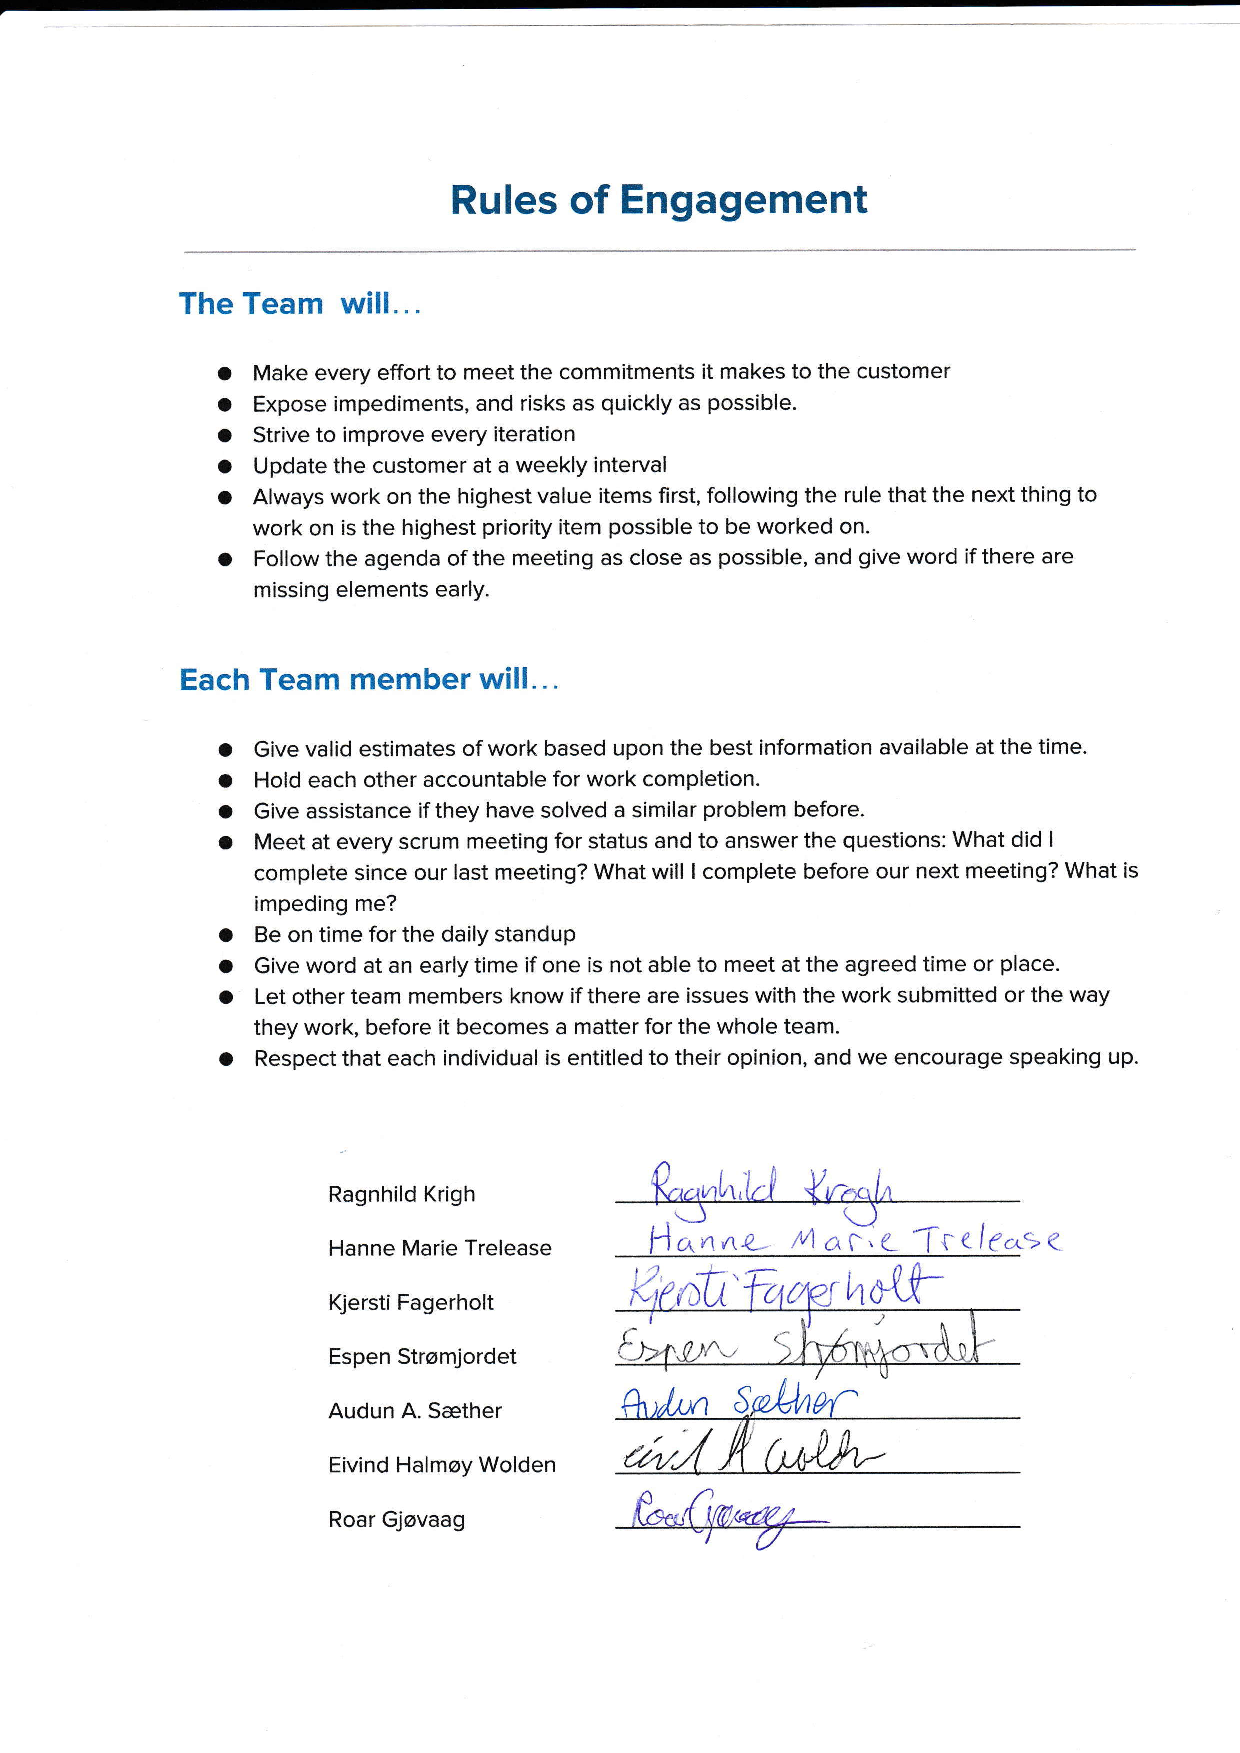
\includegraphics[trim=3cm 3.5cm 1.5cm 3cm,clip,height=13.9cm, width=11cm]{pdffig/RulesOfEngagement}
	\caption{Rules of engagement document}
	\label{fig:rules_of_engagement}
\end{figure}

\chapter{Risk list}
%$\\[0.5cm]$
\label{app:risklist}

L: Likelihood (1-9)\\
I1: Impact (1-9)\\
I2: Importance (Likelihood * Impact)\\
\small
\begin{longtable}{ | p{4.5cm} | p{1cm} | p{1cm} | p{1cm} | p{4.5cm} | p{4.5cm} |}\caption{Risk list}\label{Tab:risklist}\\
	\hline
	\textbf{Description} & \textbf{L} & \textbf{I1} & \textbf{I2} & \textbf{Preventive action} & \textbf{Remedial action} \\ \hline\endhead
	
	
	Underestimate the time planned to use for assignments & 8 & 8 & 64 & Estimate a little higher. Continuous meetings. Continuous status update on tasks & Extra work hours and help each other. Have a clear prioritization of tasks so that some less important tasks can be delayed if needed. \\ \hline
	
	The group does not deliver updated information on the report and cannot maximize the quality of the feedback obtained from the supervisor & 6 & 7 & 42 & Always make sure the report meet the demands upon delivery & Ask concrete questions to the supervisor or other competent acquaintances of the group members \\ \hline
	
	An issue in the code that is not understood or can not be fixed. & 5 & 8 & 40 & Comment on the code, and talk with each other about the work done on the code & Get help from the supervisor or other people involved. \\ \hline
	
	The group does not receive quality feedback from supervisor & 6 & 6 & 36 & Be prepared for supervisor meetings. Prepare concrete questions and discuss issues with supervisor & Ask qualified acquaintances to read and give feedback on the report.  \\ \hline
	
	Project complexity / Project too difficult & 5 & 5 & 25 & Do not plan many complicated tasks & Downgrade demands \\ \hline
	
	Poor communication with the customer leading to misunderstandings and doubts about the progress of the project & 4 & 6 & 24 & Be well prepared for meetings by establishing an agenda for the meeting and sharing it with the customer beforehand. Establish a good customer relationship. Send email to the customer for clarification & Send email to the customer for clarification. Cooperate with customer to reprioritize tasks \\ \hline
	
	Poor communication within the group leading to misunderstandings and doubts about the progress of the project & 4 & 6 & 24 & Write meeting minutes to document decisions. Have frequent meetings where every team member explains what they have done and what they are planning to do. & Make a group decision to solve the misunderstanding \\ \hline
	
	Wrong choice of development tools & 4 & 6 & 24 & Do thorough research before deciding which tools to work with & If early in project, consider changing tools \\ \hline
	
	Absence of group member(s) over a period of time & 6 & 4 & 24 & Every member of the group should be aware of what all members are working on, so that they can step in and take over the absent person's tasks & When the progress is halted by a person's absence, other group members should take over the tasks needed for further progress \\ \hline
	
	The workload is distorted. Some members of the group work too much, while others work too little. & 5 & 4 & 20 & Continuous meetings, after every meeting the team members delegate assignments. The leader of the meeting also have to make sure that everyone gets approximately the same amount of work. & Redelegate work tasks within the group. \\ \hline
	
	Poor choice of programming language. It becomes difficult to produce the product before deadline & 2 & 9 & 18 & Good research and discussion in the group. Do not choose a language that some people in the group do not have experience with & Reevaluate non-functional requirements with the customer \\ \hline
	
	Customer changes requirements & 6 & 3 & 18 & Constant communication with customer & Use an agile development process to better adapt to changes \\ \hline
	
	Data loss & 2 & 8 & 16 & Local copy and regular backups & Restore latest available backup \\ \hline
	
	Disagreement within the group on key issues in the project & 3 & 5 & 15 & Establish ground rules regarding how to discuss key issues and how to make decisions final. Make democratic decisions & If the disagreement cannot be solved, one may involve the supervisor \\ \hline
	
	Personal conflicts between group members & 2 & 7 & 14 & Establish ground rules for the team so that emerging conflicts are solved as early as possible & First try to solve the conflict between the group members in question. If this does not work, involve the whole group. A last resort would be to involve the supervisor \\ \hline
	
	Product does not meet requirements & 2 & 7 & 14 & Request product feedback from customer & Assess which changes must be made and prioritize the most important parts to change \\ \hline
	
	Overestimate the time planned to use for assignments & 3 & 4 & 12 & Investigate the assignments so it is clear what they include, and how much effort it would take to perform them. & When the assignment is done long before the estimated time, use the extra time on the more time consuming assignments. \\ \hline
	
	Missing deadlines & 1 & 8 & 8 & Have frequent meetings and plan well & Do extra work hours to finish the work as quickly as possible \\ \hline
	
	Product is not user-friendly & 3 & 2 & 6 & Perform usability tests & Assess which changes must be made and prioritize the most important parts to change \\ \hline
	
	Technical issues(server down) & 2 & 3 & 6 & & Use the backup \\ \hline
\end{longtable}

\noindent
\chapter{Requirements}
\label{app:requirements}
\label{app:functional_requirements}

\renewcommand{\arraystretch}{2}
\begin{center}
	\small
	\begin{longtable}{ | p{1cm} | p{3cm} | p{5cm} | p{1.5cm} | p{2.5cm} | p{3cm} | }
	\caption[Functional requirements]{The requirements listed up and  prioritized by the customers wishes} \\
	
	\hline {\bf ID} & {\bf Name} & {\bf Description} & {\bf Priority} & {\bf Use Case Ref.} & {\bf Comments}\\ \hline
		\hline
		\multicolumn{6}{| >{\columncolor[gray]{0.8}}c |}{General}	\\\hline			
		R1 &  Language & The documentation should be written in English. The application will be written in Norwegian and the stories from Digitalt fortalt will appear as they are, most of them in Norwegian. & H  &  &  A non-functional requirement \\\hline
		
		R2& Cross-platform & The application should run on both Android and iOS. & H &  & A non-functional requirement 	\\\hline
		
		R3& Cross-platform design & The application design should appear similar on both Android and iOS. & H &  & A non-functional requirement\\\hline
		\pagebreak
		\hline
		\multicolumn{6}{| >{\columncolor[gray]{0.8}} c |}{Sign up /Sign in view}	\\\hline			
		
		R4& User recovery & The application should provide the opportunity for the user to enter email address, which then becomes the user identifier in the system from the user's point of view. & H & U1,U2 & This means that the user can access the profile from different devices.		\\\hline
		
		R5& Anonymous sign in & The application should provide the option to enter the application without registering a user by mail address.  & H & U1 & Device remembers user. User got id in database, but not mail\\\hline
	
		R6& Demo view & It should be possible to run the application mode in a demo view where the system cannot identify the user & L &  &				\\\hline
		
		R7& Personal info & The application should obtain some personal info about the user, such as age group and gender. & H & U3 & Only for research purposes \\\hline
		
		\multicolumn{6}{| >{\columncolor[gray]{0.8}} c |}{Preferences/Settings}	\\\hline
		
		R8 & Initial specification of preferences & 
		The user should be asked to set preferences in the startup process. & H & U3 &  \\\hline
		
		R8A & Set category preference & 
		The user should be asked to enter a number of preferred categories. & H & U3 &  \\\hline
		
		R8B & Set location preference & 
		The user should be asked to specify a preferred location. & L & U3 &  \\\hline
		
		R8C & Set notification preferences & 
		The user should be asked to set some preferences about notifications & L & U3 &  \\\hline
		 
		R9&	Changing preferences&  The application should provide a settings view where the user can change the preferences. & H & U9 &	\\\hline
		
		\multicolumn{6}{| >{\columncolor[gray]{0.8}} c |}{Main view: Browse recommended stories}	\\\hline
		
		R10& 
		Show list of recommended stories & The application should provide the user with a list of recommended stories based on the set preferences. The stories is presented by a picture and a short text harvested from Digitalt fortalt. & H & U4  &\\\hline
		R11& Recommend story outside user's preferences  & The application should once in a while recommend a story outside the user comfort zone, i.e. a story that the recommender algorithm does not pick out. & M &  & Purpose: To broaden the user's horizon. The purpose is not to test the algorithm\\\hline		
		
		R12& Make decision about story  & The application should provide the user with three options regarding each recommended story: to choose to read the story now, to reject the story or to save the story for later & H & U4 &\\\hline
		
		\multicolumn{6}{| >{\columncolor[gray]{0.8}} c |}{Story view}	\\\hline
		
		R13& Present story & The application should present the chosen story in a specific story view.The presentation of the story should be in accordance with the presentation on Digitalt fortalt. & H & U6 &\\\hline				
	
		R14& Give feedback / rating on story  & The application should provide the user with the opportunity to rate the story. The rating is in the form of a star system with 5 stars.  & H & U7 &\\\hline
				
		R15 & Bookmark story  & The user should be given the opportunity to connect a story to bookmarks. The bookmarks could be predefined by the system, like "Les senere" or defined by the user & M  & U5 &\\\hline
		
		R16& Link to Digitalt fortalt  & Every story should include a link to the corresponding story on Digitalt fortalt. & H & U6 &	\\\hline
		
		R17& Explain why a story was recommended & The application should provide an explanation why a given story was recommended. & H & U4 & Could just be a general statement like: "Other users who liked similar stories to you, also liked this one"\\\hline
		
		\multicolumn{6}{| >{\columncolor[gray]{0.8}} c |}{List view}	\\\hline
		
		R18& Show stories connected to a bookmark in a list & The application should show a list of bookmarked stories for each bookmark. The stories is presented by a picture and a short text. & M &  U8 &		\\\hline
		
		R19& Choose bookmark & The application should provide the user with the opportunity to choose different bookmarks. Bookmarks include: to-read,read and user-defined bookmarks & M & U8 &\\\hline
		
		\multicolumn{6}{| >{\columncolor[gray]{0.8}} c |}{Notifications}	\\\hline
		
		R20& Notifications outside the application & The application should send a notification to the user's device at the time specified in the preferences  & L &  &	In agreement with the customer this requirement will not be met			\\\hline
		
		R21& Notifications inside the application & The application should create a notification after a defined amount time to remind the user of stories that have been read but not rated & L &  & In agreement with the customer this requirement will not be met\\\hline
		
		\multicolumn{6}{| >{\columncolor[gray]{0.8}} c |}{About app}	\\\hline
		
		R22 & About the application  & The application should include an about section, which should include basic info about the project. This include references to TAG CLOUD. & H  & U10 &\\\hline
	
		\multicolumn{6}{| >{\columncolor[gray]{0.8}} c |}{Quick tour}	\\\hline
	
		R23A & Quick tour at start up & The application should provide a new user with an explanation of the application at start up.
		& H &  & \\\hline
		
		R23B & Quick tour in menu & The application should provide the opportunity to revisit the quick tour via the menu.
		& L &  & \\\hline
		
		\multicolumn{6}{| >{\columncolor[gray]{0.8}} c |}{Personalization}	\\\hline
		
		R24& Use content-based filtering & The application should use content-based filtering to recommend stories to user initially. This should in particular be based on category preferences. & H  &  & Implement this before R25. \\\hline
		
		R25& Use collaborative filtering & The application should collaborative filtering to recommend stories when the user base is large enough for the algorithm to be effective. & H  &  &\\\hline
		
		\multicolumn{6}{ | >{\columncolor[gray]{0.8}} c |}{Research}	\\\hline		
		
		R26& Gather data to SINTEF for research & The application should gather and store information about the use. This include frequency of use, success rate of recommendations and perhaps other things.  &  &  & Detailed list of what this included provided in mail from the customer. The customer will view this data through the database \\\hline
		
	\end{longtable}
\end{center}
\pagebreak

\chapter{Project Management}
\label{app:project_managment} 

\begin{comment}
\section{WBS Description}
\label{app:wbs_description}


\begin{itemize}
	\item \textbf{Project Management}
	\begin{itemize}
		\item \textbf{Method} \newline
		How does the team work, what kind of development process is used
		\item \textbf{Product Backlog} \newline
		What is to be produced, and estimation of its costs. Maintained on Trello
		\item \textbf{Risk Management} \newline
		What are the project's risks and what is done to counter/prevent them? 
		\item \textbf{Tools} \newline
		What tools are needed to execute the project.
		\item \textbf{Schedule} \newline
		When does the team meet, customer meetings, etc.
		\item \textbf{Rules of Engagement } \newline
		What are the team’s core principles
	\end{itemize}
	\item \textbf{Analysis}
	\begin{itemize}
		\item \textbf{Requirement Specification} \newline
		Specify what the product should be used for
		\begin{itemize}
			\item \textbf{Scenario} \newline
			Describing ways to use the product and in what context
			\item \textbf{Use-Case} \newline
			Describing ways to interact with the product
			
		\end{itemize}
		\item \textbf{Functionalities} \newline
		Define the functionalities of the system
		\item \textbf{Non-Functional Specifications} \newline
		Define the system’s non-functional dependencies	
		\item \textbf{Past Work} \newline
		How does the past work affect this project, what is to be reused and copied	
		\item \textbf{Algorithms} \newline
		What algorithms are of use to the personalization	
		\item \textbf{Framework} \newline
		What framework should be used for the cross-platform development
	\end{itemize}
	\item \textbf{Design}
			\item \textbf{User Interface} \newline
			What should the application look like
			
			\begin{itemize}
				\item \textbf{Concept} \newline
				Making a mockup and iterating
				
				\item \textbf{Prototypes} \newline
				Finalizing the mockup into a prototype to test on customer/users
				
				\item \textbf{IOS} \newline
				What are the distinctions between the systems
				\item \textbf{Android} \newline
				What are the distinctions between the systems
			\end{itemize}
			\item \textbf{System Modeling} \newline
			Top-level software design
			
			\begin{itemize}
				\item \textbf{Architecture} \newline
				How is the system built, how does the component fit together
				\item \textbf{Documentation} \newline
				Detailed software design
				
			\end{itemize}
			\item \textbf{Database Modeling} \newline
			Model how the database should work
			\begin{itemize}
				\item \textbf{Documentation} \newline
				Detailed database design
			\end{itemize}
	\item \textbf{Development}
			\item \textbf{Back-end} \newline
			\begin{itemize}
				\item \textbf{Database} \newline
				Implementing a database
				\item \textbf{Harvesting} \newline
				Harvest the data from Digital Fortalt
				
				\item \textbf{Personalizing } \newline
				Main objective for the project
				\begin{itemize}
					\item \textbf{Collaborative Filtering} \newline
					Filter content on the basis of other users
					\item \textbf{Content-based Filtering} \newline
					Filter content on the basis of you past feedback
				\end{itemize}
				\item \textbf{Server} \newline
				Getting the server up and running managing reboots and updates
				\item \textbf{Front-end Communication} \newline
				How should the system communicate with front-end
				\item \textbf{Research Data} \newline
				I what way would the research data be recorded and saved
				\item \textbf{Feedback} \newline
				Handling feedback
				\begin{itemize}
					\item \textbf{Bug-fixing} \newline
					Setting a side time for fixing bugs
					\item \textbf{Customer Adjustment} \newline
					Be ready for requirement modifications and small adjustments on functionalities
				\end{itemize}
			\end{itemize}
			\item \textbf{Front-End} \newline
			\begin{itemize}
				\item \textbf{IOS / Android} \newline
				\begin{itemize}
					\item \textbf{Onboarding} \newline
					Make a introduction for the application
					\item \textbf{List} \newline
					Make stories viewable in a list 
					\item \textbf{Login} \newline
					Login view
					\item \textbf{Story} \newline
					Presenting a story in accordance with the source
					\item \textbf{Recommendation } \newline
					View to present the recommendations 
					\item \textbf{Settings} \newline
					View for changing the personal settings
				\end{itemize}
				\item \textbf{Research Data} \newline
				Log and send the research data
				\item \textbf{Feedback} \newline
				Accommodate user feedback and customer feedback 
				\begin{itemize}
					\item \textbf{Bug-fixing} \newline
					Setting a side time for fixing bugs
					\item \textbf{Customer Adjustment} \newline
					requirement modifications and UI adjustments.
				\end{itemize}
				\item \textbf{Back-end Communication} \newline
				Set up communication with back-end
			\end{itemize}
	\item \textbf{Testing}
		\begin{itemize}
			\item \textbf{Unit Testing} \newline
			Complete unit test on as many function as feasible 
			\item \textbf{Component Testing} \newline
			Complete component testing on relevant modules and components 
			\item \textbf{Integration testing} \newline
			Test the integration between the modules
			\item \textbf{System testing} \newline
			Test the system as a whole
			\item \textbf{User Testing } \newline
			Test the application on potential users 
			\item \textbf{Acceptance testing} \newline
			Preform a acceptance test on the customer 
		\end{itemize}
	\item \textbf{Documentation}
		\begin{itemize}
			\item \textbf{Theory} \newline
			Find relevant theory for the project 
			\item \textbf{Commenting} \newline
			Well commented code 
			\item \textbf{Justification} \newline
			Justify decisions 
			\item \textbf{Logging} \newline
			Log meeting, activities and work hours
			\item \textbf{Licensing} \newline
			Update and write about the licensing deal, on repositories and other relevant places 
		\end{itemize}
\end{itemize}
\end{comment}

\section{Status report example}
\label{app:status_report}

Status report week 6\newline


		\textbf{Introduction} \newline
		This week has mostly been spent organising and making decisions that will impact the whole project.\newline
		
		\textbf{Progress summary} \newline
		The decisions that have been made will decide how the work is distributed in the coming weeks. Work has been made on defining goals and milestones. Furthermore, some of the tools to complete the given tasks have been found.\newline
		
		\textbf{Open / closed problems}\newline
		Closed problems:
		\begin{itemize}
			\item A cross-platform framework have been chosen.
			\item A rough estimate of what needs doing, how long it will take and when it is due has been performed in the form of a product backlog.
			\item A list of functional requirements have been compiled after a discussion with the customer.
			Use case diagrams and scenarios have been made.
			\item Justification on some of the choices made so far have been written for the report:
			\begin{itemize}
				\item Scrum
				\item Framework
			\end{itemize}
			\item Complete a WBS chart.
			\item A rules of engagement have been signed, this helps solidify what is expected of every member in the group.\newline
		\end{itemize}
		
		Open problems:\newline
		No specific ongoing problem at the end of this week.\newline
		
		Choosing a cross-platform framework was a difficult process for various reasons. There is not much experience in the group using such tools. Additionally there was an internal debate about what is expected from the customer and what does the team expect the end product to look like. This was discussed in light of the the constraints imposed from various aspects. However, the team members now feel confident that an appropriate tool have been chosen and are aware of some limitations this leads to.\newline
		
		Understanding properly what the customer wants and prioritizes has also been a focus this week. While this sounds easy enough, the technical details are often lost in communication. This is something that will require constant feedback and monitoring so that the project stays on track in regards to what is desired by the customer.\newline
		
		\textbf{Planned work for next period}\newline
		\begin{itemize}
			\item Familiarization with the chosen framework.
			\item Familiarization with digitaltfortalt.no API.
			\item Creating a design prototype is a goal, this will unify the group and make sure all members are working towards the same goal. Furthermore, this will explore what options there are and highlight any basic flaws in design.
		\end{itemize}
\raggedbottom
\newpage

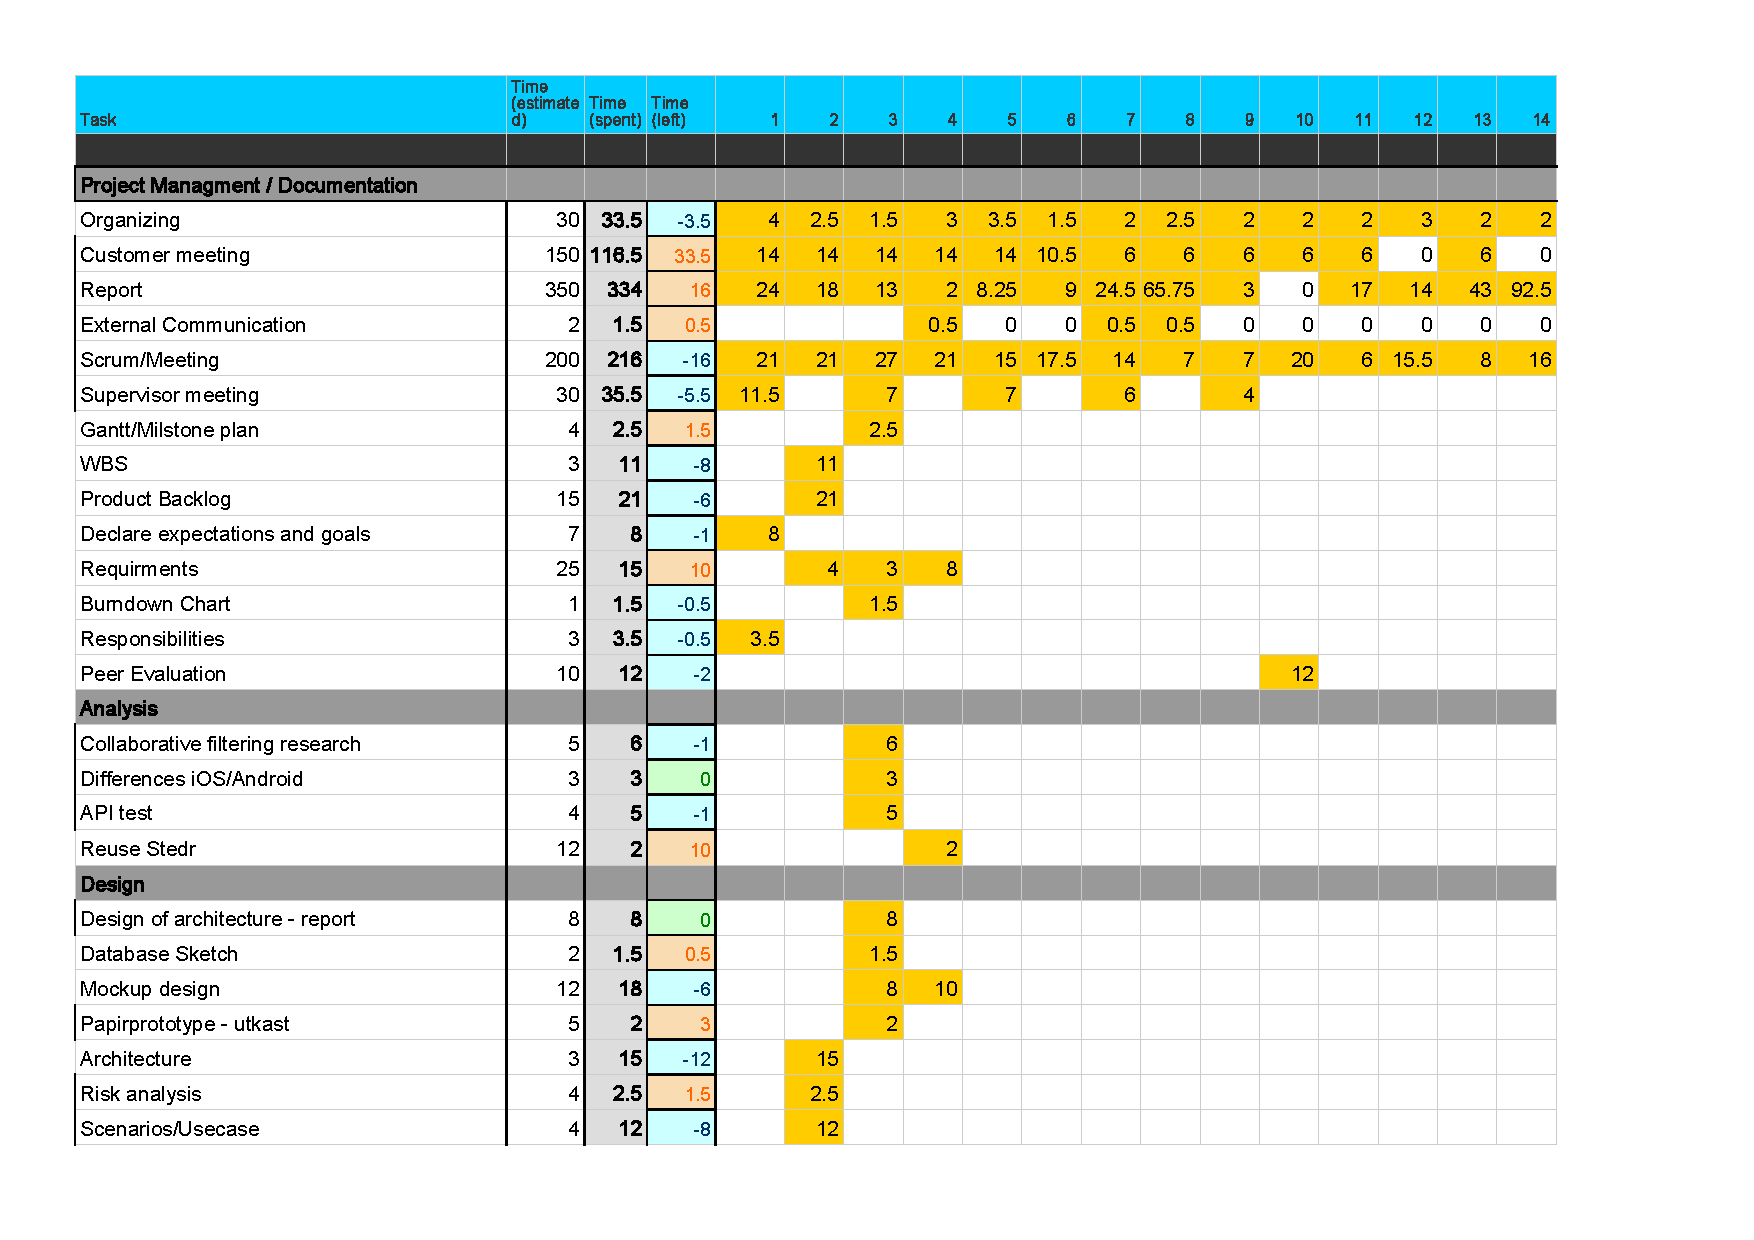
\includepdf[pages=1, pagecommand=\section{Product backlog}\label{app:product_backlog}, scale=0.9, angle=-90, offset=0cm -1.3cm]{pdffig/sprintBurndownChart}
\includepdf[pages=2-3, scale=1, angle=-90]{pdffig/sprintBurndownChart}

\chapter{Testing}		

\section{Unit test cases}
\label{app:unittest}
\renewcommand{\arraystretch}{2}%
\begin{center}
	\small
	\begin{longtable}{ | p{1.4cm} | p{5.5cm} | p{4cm} | p{4.5cm} | p{1.8cm}|}
		\caption[Unit test cases]{ Unit test cases presented by a testId, description of how the test should be performed, what input data to use and expected results.} \label{Tab:unittestcases}\\
		
		\hline {\bf Test case ID} & {\bf Description} & {\bf Input data} & {\bf Expected results} & {\bf Result}\\ \hline
		
		\multicolumn{5}{| >{\columncolor[gray]{0.8}} c |}{Unit 1: Database Helper}	\\\hline
		
		
		UN1.1 & Update one rating value in the database & Random userId, random storyId, updateValue: 2 & The function should return true when running the database request. & Pass \\\hline
		
		UN1.2 & Update rating values in the database & Random userId, random storyId, update Value : 5 & The function should return true when running the database request & Pass\\\hline
		
		UN1.3 & Update new tag\footnote{A tag is equivalent to a bookmark. Because of references to variable names such as tagName, this has not been changed in this section.} that user have created & Random userId, tagName: 'NyTestTag2' & The function should return true when running the database request& Pass \\\hline
		
		UN1.4 & Update a user's tag which is connected to a story & Random userId, Random storyId, tagName: 'Les senere' & The function should return true when running the database request& Pass \\\hline
		
		UN1.5 & Update a user's action of rejecting a story & Random userId, Random storyId & The function should return true when running the database request & Pass \\\hline
		
		UN1.6 & Update a story as recommended & Random userId, Random storyId & The function should return true when running the database request & Pass\\\hline
		
		UN1.7 & Get rating on a story done by a user  & Random userId, Random storyId & Should return row with the rating presented as a integer & Pass\\ \hline			
		
		UN1.8 & Get the predefined tags connected to a user & Random userId & Should return row with the tags "Les senere" and "Les" which all users in the system is connected to. If this user has self made tags, they should be included & Pass\\ \hline
		
		UN1.9 & Get all the tags connected to a user & Specified userId: 105 & Should return row with the tags "Les senere" and "Les" which all users in the system is connected to, included the added tag 'NyTestTag' & Pass\\ \hline
		
		UN1.10 & Get the tags connected to a story and a user & Specified userId: 105, specified storyId: 'DF.1295' & Should return row with the tag 'NyTestTag' & Pass \\ \hline
		
		UN1.11 & Get stories with timestamp & -  & Should return rows with 167 storyId and a timestamp which indicate when the story was last changed & Pass \\ \hline
		
		UN1.12 & Get subcategories to a specific story & Random storyId & Should return a row with an array of subcategory Ids & Pass\\ \hline
		
		UN1.13 & Get story information & Specified userId: 105, specified storyId: 'DF.5220' & Should return row with an array with the keys: userId, storyId, explanation, rating, false\textunderscore recommend, recommended\textunderscore ranking, in\textunderscore front-end\textunderscore array, estimated\textunderscore Rating & Pass  \\ \hline
		\multicolumn{5}{| >{\columncolor[gray]{0.8}} c |}{Unit 2: Database Story}	\\\hline			
		
		UN2.1 & Fetch story & Specified storyId: 'DF.1812', specified userId: 105 & Should return row with an array of the categories to the story and tags and tagName that are connected to the userId  & Pass\\ \hline
		
		UN2.2 & Get recommended stories for a user & random userId &  Should return 10 rows with stories, and they should include: userId, storyId, recommended\textunderscore ranking, explanation, false\textunderscore recommend, title, introduction, author, categories and mediaId & Pass\\ \hline
		
		UN2.3 & Get list of stories which is tagged by a user & Specified userId: 103, tagName: 'NyTestTag' & Should return rows with stories, and they should include: storyId, title, author, introduction, date, tagName, categories and mediaId & Pass\\ \hline
		
		UN2.4 & Get subcategories per story & - & Should return 167 stories  with numericalId and subcategory ids  & Pass\\ \hline
		
		UN2.5 & Get all stories with storyId, numericalId and categories & - & Should return 167 rows with storyId, numericalId and categories & Pass\\ \hline
		
		UN2.6 & Get states per story  & Specified userId: 258, specified storyId: 'DF.1600'& Should return a row with stateId, numTimesRecorded and latestStateTime &  Pass\\ \hline
		\multicolumn{5}{| >{\columncolor[gray]{0.8}} c |}{Unit 3: Database User}	\\\hline
		
		
		UN3.1 & Add user   & example mail: example@example.com & Should return a userId that is not null &  Pass\\ \hline
		
		UN3.2 & Get user from Id & UserId: generated new Id. & Should return a userId from the database which is equal the userId input & Pass\\ \hline
		
		UN3.3 & Update user e-mail &UserId: generated new id,\newline e-mail: newmail@example.com &  Should return a e-mail from the database which is equal the e-mail input & Pass\\ \hline
		
		UN3.4 & Update user age & UserId: generated new Id ,\newline age group: 0 & Should return a user model from the database, which includes the age group that is equal to the age group input.  & Pass\\ \hline
		
		UN3.5 & Update user categories & UserId: generated new id, \newline category preference: [2] & Should return a row with user model from the database with the category preference that is equal to the category preference input.  & Pass\\ \hline
		
		UN3.6 & Get user from e-mail & UserId: generated new id, \newline email:54@example.com & Should return a user model from the database, which includes the e-mail that is equal to the e-mail input.   & Pass\\ \hline							
		
		UN3.7 & Get user categories & UserId: generated new id, \newline category preferences: [1,3,5,7,9] & Should return the categories from the database that is equal to the category preferences input  & Pass\\ \hline
		
		UN3.8 & Get user e-mail from Id  & UserId: generated new id  &  Should return a  user model from the database,which includes the e-mail that is equal the e-mail input. & Pass\\ \hline
		\pagebreak
		\hline
		\multicolumn{5}{| >{\columncolor[gray]{0.8}} c |}{Unit 4: User Model}	\\\hline
		
		UN4.1 & Initiate User   & userId:1, \newline mail: example@example.com & Should create a user model with the correct input. The getters should return the values that matches with the input values& Pass\\ \hline
		
		UN4.2 & Set all user details &userId:1, \newline mail: example@example.com,gender: 0, age group: 1, use of loc. : 0 , category preference: [1,3,5,7,9] & Should add the correct user details to the user model. The getters should return the values that matches with the input values  & Pass\\ \hline
		
		UN4.2 & Print all  &  userId:1, \newline mail: example@example.com,gender: 0, age group: 1, use of loc. : 0 , category preference: [1,3,5,7,9] & The printAll function should return a string with all the correct attributes and values that matches the input values .   & Pass\\ \hline
		
		\multicolumn{5}{| >{\columncolor[gray]{0.8}} c |}{Unit 5: Compute Preference Value}	\\\hline
		
		
		UN5.1 & Compute preference value for all stories for a  user & Random userId & Should return 167 rows from the database, and every row should include: storyId, userId, numericalId and preferenceValue  & Pass\\ \hline
		
		UN5.2 & Compute preference value of a story for a user  & Random userId , specific 'DF.1098' & Should return an array with userId, storyId, numericalId and the preference value& Pass\\ \hline
		
		UN5.3 & Compute preference value & Specific storyId  & Should return the preference value which is the type double & Pass\\ \hline
		
		
		
		
		\multicolumn{5}{| >{\columncolor[gray]{0.8}} c |}{Unit 6: Recommendation}	\\\hline
		
		UN6.1 & Run recommender & Random userId  & & Pass\\ \hline	
		
		UN6.2 & New content-based recommendation & Input: setUp.xml - a data model with userIds and connected preference values. & The recommender should return the correct number of recommendations when it should create new ones &  Pass\\ \hline			
		
		UN6.3 & Add content-based recommendation & Input: setUp.xml- a data model with userIds and connected preference values. & The recommender should return the correct number of recommendations when its adding recommendations to existing ones & Pass\\ \hline	
		\hline
		\multicolumn{5}{| >{\columncolor[gray]{0.8}} c |}{Unit 7:  Database connection with Java}	\\\hline
		
		UN7.1 & Insert recommendation  & userId: 1,\newline  storyId: Df.1098,\newline DF.1501,\newline explanation: 0, \newline false\textunderscore rec. :0, \newline ranking: 3,4,\newline estimatedValue: 0,0 & Expected table in XML-representation(insert-expected.xml) is the same as the actual from the database & Pass\\ \hline			
		
		UN7.2 & Insert and update  & userId: 1, \newline storyIds: DF.1709,DF.1849, \newline explanation:“updated”, \newline false\textunderscore rec. : 1,0, \newline typeoffrec. :1,1, \newline  ranking: 3,4 estimatedValue: 4.5, 2.5   & Expected table in XML-representation(insertUpdate-expected.xml) is the same as the actual from the databas & Pass\\ \hline										
		
		UN7.3 & Delete recommendations & UserId: 1 & Expected table in XML representation(delete-expected.xml)  is the same table returned from DB & Pass\\ \hline		
		
		UN7.4 & Rated  & UserIds: 3,5 \newline	numericalId: 1812,1901 & The getRated function should fetch the correct stories. The input rating should be the same as the returned ratings & Pass \\ \hline						
		UN7.5 & Test front-end array & Numerical Ids: 1849, 1901  & Get stories from front-end array should match the front-end array in XML format(setUp.xml) & Pass\\ \hline	
		
		UN7.6 & Create explanation  & Numerical Ids: 1098,1115,1501  & The create explanation function should return a string with the correct storyIds and their titles. & Pass\\ \hline								
		\pagebreak
		\hline
		\multicolumn{5}{| >{\columncolor[gray]{0.8}} c |}{Unit 8: UI-Log in}	\\\hline			
		
		UN8.1 & Log in with an already existing user\newline - Check if response is correct & existinguser@\newline mail.no & The user should get access and be directed to the recommendation view(main view) & Pass \\ \hline			
		
		UN8.2 & Log in with a non-existing user \newline - Check if response is correct & “newemail@\newline gmail.com” & The user should get access and be directed to the setup view.& Pass \\\hline	
		
		UN8.3 &  Login a user with the wrong e-mail format \newline - Check if response message is correct & “newemail” & The user should not get access and get a textual response from the system that the format of the input is wrong.& Pass\\ \hline	
		\hline
		\multicolumn{5}{| >{\columncolor[gray]{0.8}} c |}{Unit 9: UI-Story View}	\\\hline			
		
		UN9.1 & If story contains sound clip or video, check if these are presented properly & - story with video\newline
		-story with sound clip & Should show the presence sound clip and video in the tabs. Should be able to handle the different video types, and be able to play them. & Pass \\ \hline			
		
		UN9.2 & Give a rating\newline - Check if the stars change color and response message are visible to the user.  & & Stars should change color when user performs rating, and the user should get a response message from the system which says that this story has been rated. & Pass \\\hline	
		
		UN9.3 & Give the story a new bookmark with a name\newline -add this \newline -Check if response message is visible to the user  & “new bookmark”  & When a new bookmark is made and the story is stored here, the user should get response message about this.& Pass\\ \hline	
		\hline
		\multicolumn{5}{| >{\columncolor[gray]{0.8}} c |}{Unit 10: Settings}	\\\hline					
		
		UN10.1 & Update profile with the wrong e-mail format  & updateemail  & The user should get a response message from the system that the input was not valid and that the user should try again. & Pass  \\ \hline
		
		UN10.2 & Update profile with a e-mail that already exists in the system  & “alreadyexistingemail\newline @email.com”  & The user should get a response message from the system that the input was not valid and that the user should try again.   & Pass \\\hline	
		
		
	\end{longtable}
\end{center}
\raggedbottom
\newpage		


\section{Integration test cases}
\label{app:integrationtest}


\renewcommand{\arraystretch}{2}%
\begin{center}
	\small
	\begin{longtable}{ | p{1cm} | p{5.5cm} | p{4cm} | p{4.5cm} | p{2cm}|}
		
		\caption[Integration test cases]{Integration test cases} \label{Tab:integrationtestcases}\\
		\hline
		\textbf{Test case ID} & \textbf{Description} & \textbf{Input data} & \textbf{Expected results} & \textbf{Result} \\ \hline
		
		I.1 & Simulate a HTTP request which will log in a user for the first time with an e-mail address. \newline Call getUserFromEmail to the database & e-mail: 'testnr16@example.com,\newline requestType: addUser & The HTTP request should return successful message included the newly created userId. The database  function should return a row with the userId, mail, age\textunderscore group, gender and use\textunderscore of\textunderscore location  & Pass \\ \hline
		
		I.2 & Simulate a HTTP request which will log in a user for the first time without an e-mail address. \newline Call getUserFromId to the database & e-mail:null, \newline request type:addUser  & The HTTP request should return a successful message included the newly created userId The database function should return the usermodel containing userId, mail, age\textunderscore group, gender and user\textunderscore of\textunderscore location.  & Pass \\ \hline
		
		I.3 & Simulate a HTTP request which will update a users profile. \newline Call getUserFromId to the database.  \newline Check if the updates where correct & e-mail: 'testMail23@example.com', request type: updateUser,  & The HTTP request should return a successfull message. The database function should return a usermodel where the e-mail match the input.& Pass\\ \hline
		
		I.4 & Simulate a HTTP request that will create a new test user without an e-mail. Simulate another HTTP request which will update e-mail to this test user, with an email that already exists in the system \newline  Call the getUserFromId function to the database. \newline Check if the user is not updated & e-mail: 'testMail23@example.com' & The HTTP request should return a failure message. The database function should return an usermodel where the e-mail is null. & Pass\\ \hline
		
		I.5 & Simulate a HTTP request that will create a new test user without an e-mail. \newline Simulate another HTTP request which will update e-mail to this test user \newline  Call the getUserFromId function to the database. \newline Check if the user is updated &  & The HTTP request should return a successful message. The database function should return an usermodel where the e-mail matches the input. & Pass\\ \hline
		
		I.6 & Simulate a HTTP request that will create a new test user with an e-mail\newline  Simulate another HTTP request that will return the user model from the users e-mail \newline Check if the returned data has all attributes required, and that the data match with the input data & e-mail: 'getUserFromEmailTest@example.com",\newline request type: addUser/getUserFromEmail  & The HTTP request should return a usermodel with the attributes userId, e-mail, age\textunderscore group, gender, use\textunderscore of\textunderscore location and with the data which match the input data.& Pass \\ \hline
		
		I.7 & Simulate a HTTP request that will create a new test user without an e-mail.\newline  Simulate another HTTP request that will return the user model from the users id. \newline Check if the returned data has all attributes required, and that the data match with the input data & e-mail: null,\newline request type: addUser/getUserFromId  & The HTTP request should return a usermodel with the attributes userId, e-mail, age\textunderscore group, gender, use\textunderscore of\textunderscore location and with the data which match the input data. & Pass\\ \hline
		
		I.8 & Simulate a HTTP request that will create a new test user without an e-mail. \newline Call the getNumberOfRatingsDoneByThisUser to the database. \newline  Simulate another HTTP request which will connect a rating to a story for this user.  \newline Call the getNumberOfRatingsDoneByThisUser to the database again \newline Check if another rating is registered & e-mail: null,\newline request type: rating, storyId: 'DF.52201, random userId  & The HTTP request should return a usermodel with the attributes userId, e-mail, age\textunderscore group, gender, use\textunderscore of\textunderscore location and with the data which match the input data. & Pass \\ \hline
		
		%THIS IS NOT DONE YET
		I.9 & Simulate a HTTP request that will create a new test user without an e-mail. \newline  \newline  Simulate another HTTP request where the user rejects a story.  \newline  \newline Check if the rejection is stored & e-mail: null,\newline request type: rejectStory  &  & Pass \\ \hline
		
		I.10 & Simulate a HTTP request that will create a new test user without an e-mail. \newline  Simulate a  request that will create a new tag for this user \newline Simulate a HTTP request that will return the list of tags for this user \newline Check if the new tag has been added  & request type: addUser/addNewTag/getList  tagName: 'newTag1' & The returned list should only include the one tag that where created.& Pass\\ \hline
		
		I.11 & Simulate a HTTP request that will create a new test user without an e-mail. \newline  Simulate a HTTP request that will create a new tag for this user. \newline Simulate a HTTP request that will return the list of stories contained in this taglist. \newline Check if the new tag has been added  & request type: addUser,tagStory,getList \newline tagName: 'newTag1',\newline storyId: 'DF.5223' & The returned list should have the recently added story in the top of the list. The list should have the following attributes connected to every story: id, title, description, false\textunderscore recommend, explanation, picture, thumbnail, categories, mediaType, author, data  & Pass\\ \hline
		
		I.12 & Simulate a HTTP request that will create a new tag for a user. \newline  Simulate a HTTP request that will return all the tags connected to this user. \newline Check if the tag was stored \newline Simulate a HTTP request that will remove the new tag that were created earlier \newline Simulate another HTTP request that will return all the tags connected to this user \newline Check if the new tag has been removed  & Specified userId: 105, \newline request type: addnewTag, getAllLists, removeTag,\newline tagName: 'tagToBeRemoved',\newline storyId: 'DF.6081' & The returned list should have the recently added story in the top of the list. The list should have the following attributes connected to every story: id, title, description, false\textunderscore recommend, explanation, picture, thumbnail, categories, mediaType, author, data  & Pass\\ \hline
		
		
		I.13 & Simulate a HTTP request that will return the list connected to a tag for an user  & Specified userId: 105, request type: getList,\newline tagName: 'Les senere' & Should return a list of the stories connected to this tag. The stories should have the following attributes: id, title, description, false\textunderscore recommend, explanation, picture, thumbnail, categories, mediaType, author, date & Pass\\ \hline					
		
		
		I.14 & Simulate a HTTP request that will return all the tags connected to a user  & Specified userId: 105, \newline request type: getList, \newline tagName: 'Les senere' & Should return a list of the tags. The tags should have the attributes text and checked. & Pass\\ \hline	
		
	\end{longtable}
\end{center}
\raggedbottom
\newpage		

\section{System test cases}
\label{app:systemtest}

\begin{table}[H]
	\small
	\centering
	\caption{System test case for creating a recoverable profile.}
	\begin{tabular}[b]{ | l | l  |}
			\hline
			\textbf{Test ID} & T1  \\ \hline
			\textbf{Test Item} & Create recoverable profile \\ \hline
			\textbf{Approach} & \begin{minipage}{5in}The user locate and press the “register user” button in the app. Applies the e-mail in the correct format. The response is valid and the user gets feedback. \end{minipage}\\ \hline
			\textbf{Input data} &  “newuser@example.com”\\ \hline
			
			\textbf{Expected results} & \begin{minipage}{5in}The user writes the correct e-mail address and get the correct feedback from the system: "Kontakter server" and will be directed to the startup page.\end{minipage}\\ \hline&\\[-3.8ex]
		
			\textbf{Testing task} & \begin{minipage}{5in}
			\begin{enumerate}[noitemsep]
			\item Click  “create user”-button.
			\item Apply e-mail address to the e-mail input field 
			\item Receive feedback from the system
			\item Check e-mail inbox to se if the correct mail from the system was received 
			 \end{enumerate} \end{minipage}
			\\&\\[-3.8ex] \hline
			\textbf{Depends on tests}& \\ \hline	
			\textbf{Pass/Fail} & Passed \\\hline				
		\end{tabular}
	\label{Tab:systemTesting1}
\end{table}


	\begin{table}[H]
		\small
		\centering
		\caption{System test case for login with e-mail registration}
		\begin{tabular}{ | l | l  |}
			\hline
			\textbf{Test ID} & T2  \\ \hline 
			\textbf{Test Item} & Log in with e-mail registration \\ \hline
			\textbf{Approach} & \begin{minipage}{5in}The user locate the login button, applies the registered e-mail and obtain access to the system and the profile connected to this e-mail address . \end{minipage}\\ \hline
			\textbf{Input data} &  valid email: “user@example.com”, \newline example invalid e-mail: “mail@example”\\ \hline&\\[-3.8ex]
			\textbf{Expected results} & \begin{minipage}{5in}
			\begin{itemize}[noitemsep]
				\item The first time the user have logged in: \newline System Response:  Choose preferences-view should appear.
				\item The user have done this process before: \newline System Response: "Vennligst vent mens vi finner historier vi tror du vil like" and direct the user to the view with the recommended stories.
				\item The user types an e-mail with wrong e-mail format: \newline System Response: "Ikke en gyldig adresse" 
				
			\end{itemize} \end{minipage}
			 \\ &\\[-3.8ex]\hline&\\[-3.8ex]
			\textbf{Testing task} & \begin{minipage}{5in}
			\begin{enumerate}[noitemsep]
			\item Navigate to the login view
			\item Apply e-mail address to the e-mail input field
			\item Receive response from system
			\end{enumerate}\end{minipage}
			 \\ &\\[-3.8ex]\hline
			\textbf{Depends on tests} & T1 \\ \hline					
			\textbf{Pass/Fail} & Passed \\\hline
		\end{tabular}
	
	\label{Tab_systemTesting2}
	\end{table}

	\begin{table}[H]
		\small
		\centering
		\caption{System test case for initial settings}
		\begin{tabular}{ | l | l |}			
			\hline
			\textbf{Test ID} & T3  \\ \hline
			\textbf{Test Item} & Set initial settings \\ \hline
			\textbf{Approach} & \begin{minipage}{5in}The user is logged in to the system for the first time. The user will choose age group and gender in the initial settings that will appear the first time the user is logged on to the system. After this the user will be asked to choose cultural category preferences.  \end{minipage}\\ \hline
			\textbf{Item pass/Fail criteria} & \\ \hline
			\textbf{Input data} & \begin{minipage}{5in} User action: click the buttons for the age group, gender and interests, and next buttons  \end{minipage}\\ \hline
			\textbf{Expected results} & \begin{minipage}{5in}The user will click the buttons for age group, gender, and interests. The buttons will change color when clicked on. The user navigates to next view by clicking the next button and will obtain access to the system. If the user do not select interests the user will get a response for the system that it is necessary. \end{minipage}\\ \hline&\\[-3.8ex]
			\textbf{Testing task} & \begin{minipage}{5in}
			\begin{enumerate}[noitemsep]
				\item Start app
				\item Click the correct age group and gender.
				\item Navigate to the next page
				\item Navigate to the next page without selecting interests
				\item Receive feedback from system
				\item Select two interests
				\item Navigate to the next page
			\end{enumerate}\end{minipage}
			\\ &\\[-3.8ex]\hline
			\textbf{Depends on tests} & \\ \hline	
			\textbf{Pass/Fail} & Passed \\\hline				
		\end{tabular}
	\label{Tab:systemTesting3}
	\end{table}


	\begin{table}[H]
		\small
		\centering
		\caption{System test case for browsing recommended stories}
		\begin{tabular}{ | l | l  |}
			\hline
			\hline
			\textbf{Test ID} & T4  \\ \hline
			\textbf{Test Item} & Browse recommended stories \\ \hline
			\textbf{Approach} & \begin{minipage}{5in}The user is shown a list of recommended stories. The user will click on the first story. The story will be viewed and the user closes it. 
			\end{minipage}\\ \hline
			\textbf{Item pass/Fail criteria} &  \\ \hline			
			\textbf{Input data} &  User action: click arrow\\ \hline
			\textbf{Expected results} & \begin{minipage}{5in}The view should show a list with recommended stories. The view of the stories will include a title, story picture or default picture, an introduction, category icons, media icons and a explanation of why this story is recommended to the user.  The view should show 10 more recommendations when the user have browsed through the 10 first stories in the list.
			When the user clicks a story the full story should appear in a full screen, including text and potential pictures, videos and sound clips.   \end{minipage}\\ \hline&\\[-3.8ex]
			\textbf{Testing task} & \begin{minipage}{5in}
			\begin{enumerate}[noitemsep]
			\item Click on a recommended story
			\item Locate back button and close the story
			\item Click on the next recommended story
			\item Navigate 
			\end{enumerate}\end{minipage}
			\\ &\\[-3.8ex]\hline
			\textbf{Depends on tests} & T1,T2 \\ \hline		
			\textbf{Pass/Fail} & Passed \\\hline			
		\end{tabular}
	
	\label{Tab:systemTesting4}
	\end{table}


	\begin{table}[H]
		\small
		\centering
		\caption{System test case for adding a story to list}
		\begin{tabular}{ | l | l  |}
			\hline 
			\textbf{Test ID} & T5  \\ \hline
			\textbf{Test Item}  & Add story to list	 \\ \hline
			\textbf{Approach} & \begin{minipage}{5in}The user navigate to a story and gives the story a rating. The user clicks the bookmark button in the story, and gives a name to a new list of stories.   \end{minipage}\\ \hline
			\textbf{Input data} & \begin{minipage}{5in}User action: Click on a star, Give name to a new list of stories: ex. “My Favorite Stories” \end{minipage}\\ \hline
			\textbf{Expected results} & \begin{minipage}{5in}The story that was rated with stars are automatically put in the “read” list. The story should be stored in the new list of “My Favorite Stories” and the user have access to this by navigating to the menu, and then to “Bokmerker”. \end{minipage}\\ \hline&\\[-3.8ex]
			\textbf{Testing task} & \begin{minipage}{5in}
			\begin{enumerate}[noitemsep]
			\item Click on a story in the recommendation view 
			\item Click on the star icon to in the right upper corner 
			\item Click on one of the stars in the rating view to give rate.
			\item Click out from the view. 
			\item Click the bookmark button in the story 
			\item Click the plus icon
			\item Type in a "My Favorite Stories" and click out of the view.
			\item Navigate to the lists via the menu
			\item Click on "My Favorite Stories"
			\item Click on the first story in the list
			\item Navigates to the “read” list
			\item Click on the first story in the list
			\end{enumerate}\end{minipage}
			\\ &\\[-3.8ex]\hline
			\textbf{Depends on tests} & \\ \hline			
			\textbf{Pass/Fail} & Passed \\\hline		
		\end{tabular}
	
	\label{Tab:systemTesting5}
	\end{table}
	


	\begin{table}[H]
		\small
		\centering
		\caption{System test case for giving rating}
		\begin{tabular}{ | l | l  |}
			\hline
			\textbf{Test ID} & T6  \\ \hline
			\textbf{Test Item} & Give a rating \\ \hline
			\textbf{Approach} & \begin{minipage}{5in}The user gives a story a rating by clicking the stars. The user navigates to bookmark lists and checks if the story was stored in the “read” list \end{minipage}\\ \hline
			\textbf{Input data} &  \begin{minipage}{5in}User action: clicks on story, navigated to rating view, clicks on a star. \end{minipage}\\ \hline
			\textbf{Expected results} & \begin{minipage}{5in}The star buttons that were pressed will change color.  The system should store the rating for that story. The next time the user clicks on this story - the yellow stars will show the users rating.  \end{minipage}\\ \hline&\\[-3.8ex]
			\textbf{Testing task} & \begin{minipage}{5in}
			\begin{enumerate}[noitemsep]
			\item Click on a story in the recommendation view
			\item Click on the star icon to in the right upper corner
			\item Click on one of the stars in the rating view to give rate.
			\item Click out from the view. 
			\item Click on the star icon again
			\item Close rating view
			\end{enumerate}\end{minipage}
			\\ &\\[-3.8ex]\hline
			\textbf{Depends on tests} & T1,T2 \\ \hline		
			\textbf{Pass/Fail} & Passed \\\hline			
		\end{tabular}
	\label{Tab_systemTesting6}
	\end{table}




	\begin{table}[H]
		\small
		\centering
		\caption{System test case for specifying settings}
		\begin{tabular}{ | l | l  |}
			\hline
			\textbf{Test ID} & T7  \\ \hline
			\textbf{Test Item} & Specify settings \\ \hline
			\textbf{Approach} & \begin{minipage}{5in}The user navigates to "Innstillinger" via the sidebar menu. The user then adds preferences and change the permission to use location. \end{minipage}\\ \hline		
			\textbf{Input data} &  \begin{minipage}{5in}User action: click the buttons for the age group, gender and interests. \end{minipage}\\ \hline
			\textbf{Expected results} &  \begin{minipage}{5in}The user will click the buttons for age group, gender, and interests. The buttons will change color when clicked on. The user navigates to next view by clicking the next button and the system will give the response: "Vennligst vent mens vi finner historier vi tror du vil like". 
			The system saves the users preferences and updates the recommended stories list. The list of stories should now be updated.  \end{minipage}\\ \hline&\\[-3.8ex]
			\textbf{Testing task} & \begin{minipage}{5in}
			\begin{enumerate}[noitemsep]
				\item Navigate to settings
				\item Navigate to preferences
				\item Add another preferences
				\item Check the recommended stories list to see if it is updated

			\end{enumerate}\end{minipage}
			\\ &\\[-3.8ex]\hline
			\textbf{Depends on tests} & \\ \hline		
			\textbf{Pass/Fail} & Passed \\\hline			
		\end{tabular}
	\label{Tab:systemTesting7}
	\end{table}
	
\clearpage
\section{Usability test cases}
\label{app:usabilitytest}
DNS: Desired next step with reference to the numbering in the View column\\
\renewcommand{\arraystretch}{2}%
\begin{center}
	\small
	\begin{longtable}{ | p{3.7cm} | p{1cm} | p{13cm}|}
		\caption[Usability test]{Usability test } \label{Tab:usabilityTest}\\
		\hline
		\textbf{View} & \textbf{DNS} & \textbf{Comments}
		\\ \hline
		
		\textbf{1. Intro / Tutorial} & 2 & 
		\textbf{Feedback:} Not clear if user is supposed to swipe or not. The view is lacking in content. Users do not know if they can go back between views. The users would like an introduction to the application.\newline
		\textbf{Changes:} Add animation/intro
		\\\hline
		
		\textbf{2. Login} & 3  & 
		\textbf{Feedback:} Users often click the skip button instead of logging in. The description of why users have to input their e-mail is not clear. The text is too small. The term "email verification" is not understood.\newline
		\textbf{Changes:} Change wording in the view. Make the skip button smaller to encourage logging in instead.
		\\\hline
		
		\textbf{3. Profil} & 4 & 
		\textbf{Feedback:} Some users thought this was part of the recommendation. They wonder if this is for research data or for the application.\newline
		\textbf{Changes:} Explain why age and gender information is needed. Make the default age and gender not selected so user is not forced to choose.
		\\\hline
		
		\textbf{4. Interests} & 5  & 
		\textbf{Feedback:} Users do not understand what this view is, they want an explanation. It is not clear if you can choose more than one interest.\newline		
		\textbf{Changes:} Add a better explanation.
		\\\hline
		
		\textbf{5. Media format} & 5 & 
		\textbf{Feedback:} The sound icon was interpreted as music. User did not understand what they were choosing, and how this would affect stories.\newline
		\textbf{Changes:} Remove this view, because it does not add much to the application, and users are confused about its function and meaning.
		\\\hline
		
		\textbf{6. Recommendations} & 6 & 
		\textbf{Feedback:} The read later button is not understood. Users do not understand that it places the story in a list. Users do not understand that they can swipe in this view, or what they can touch. The users feel a bit "dumped" into this view with no explanation.\newline
		\textbf{Changes:} Remove read later button and add a bookmark icon at the top right instead. Add a card deck or something else to show users that they can swipe. Add a loading animation for when the view is retrieving stories. Change the title of the view to "Anbefalte historier". Make it clear that the card can be touched and make it possible to remove the card.
		\\\hline
		
		\textbf{7. Story View} & 7 & 
		\textbf{Feedback:} Some users did not understand the bookmark icon. They did not know where to go from this view. There was also some confusion about what the "ikke interessert" button means.\newline 
		\textbf{Changes:} Add a back button. Change the name of the "ikke interessert" button. Make the icons more understandable.
		\\\hline
		
		\textbf{Story bookmark} & 8  & 
		\textbf{Feedback:} Users want to know if they can change the name of existing lists.\newline
		\textbf{Changes:} None	
		\\\hline
		
		\textbf{8. Menu} & 9  &
		\textbf{Feedback:} User does not understand what the "utforsk" button mean.\newline
		\textbf{Changes:} Change the name of "utforsk" to make it clear that this is where the main personalization view is.		
		\\\hline
		
		\textbf{9. List} & 9 \textgreater 12 &
		\textbf{Feedback:} Some users are unsure how to delete a story from a list. They try to swipe in both directions.\newline
		\textbf{Changes:} Add some hint or indicator that you can swipe. Maybe let users swipe both ways.
		\\\hline
	\end{longtable}
\end{center}


	
\chapter{Meeting report examples}
\label{app:meetingreport}

	\begin{figure}[h]
		\centering
		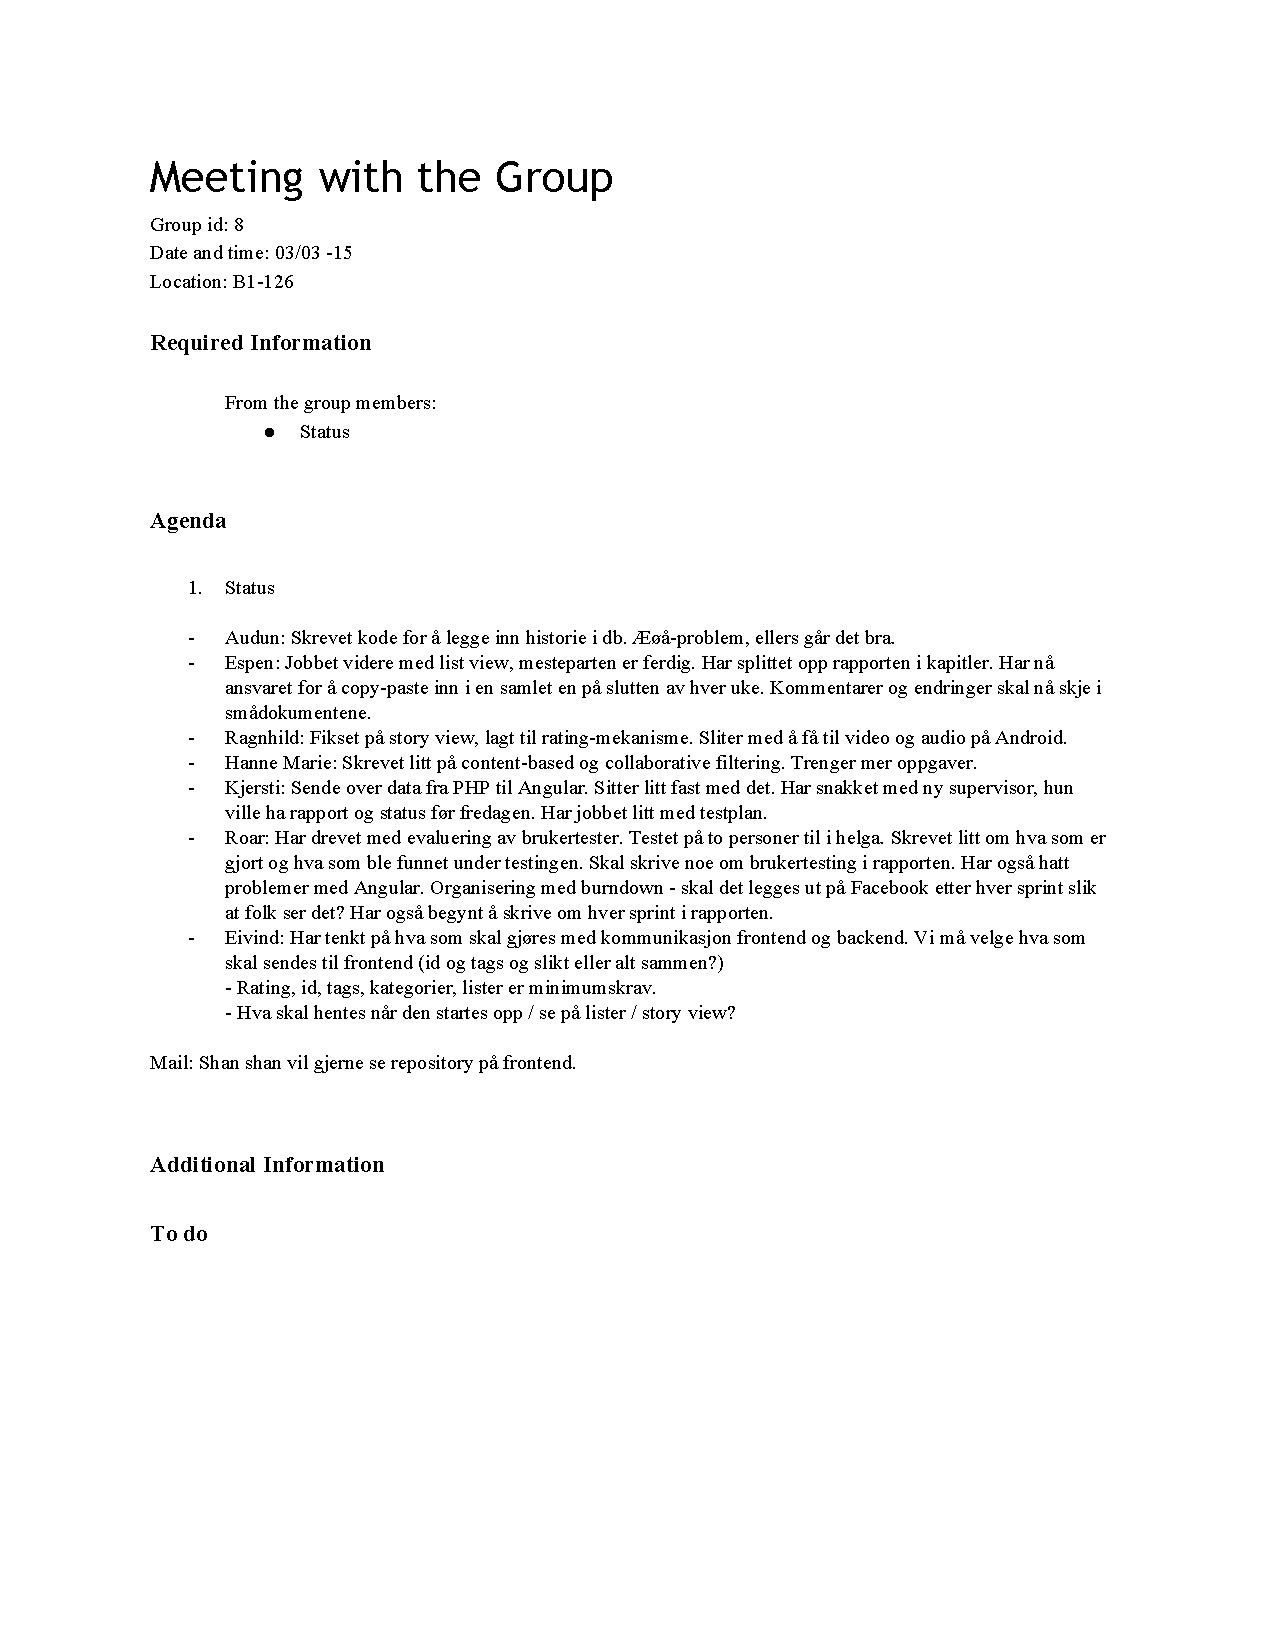
\includegraphics[trim=2.5cm 6.5cm 2cm 2.5cm,clip, scale=0.9]{pdffig/group_meeting}
		\label{app:group_meeting}
	\end{figure}
	
	%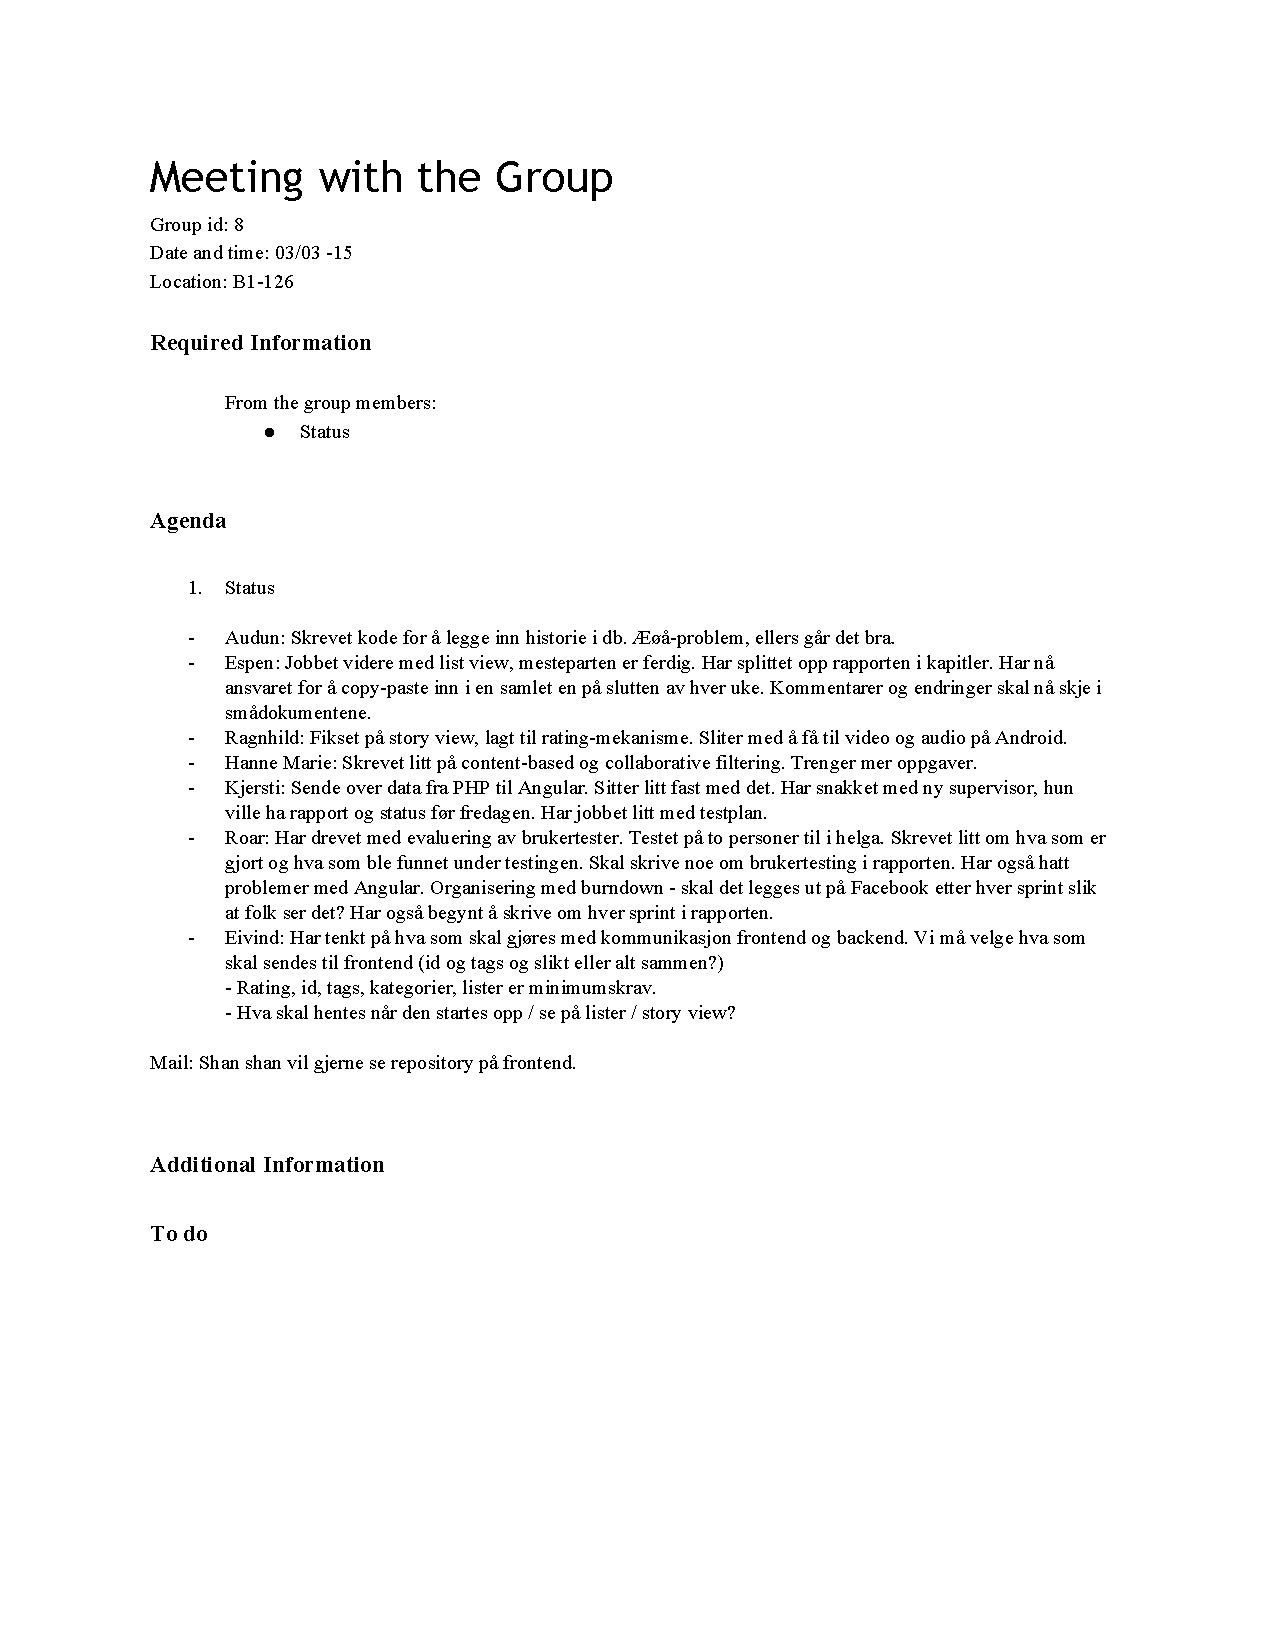
\includepdf[pages=1, pagecommand=\label{app:group_meeting}]{pdffig/group_meeting}

	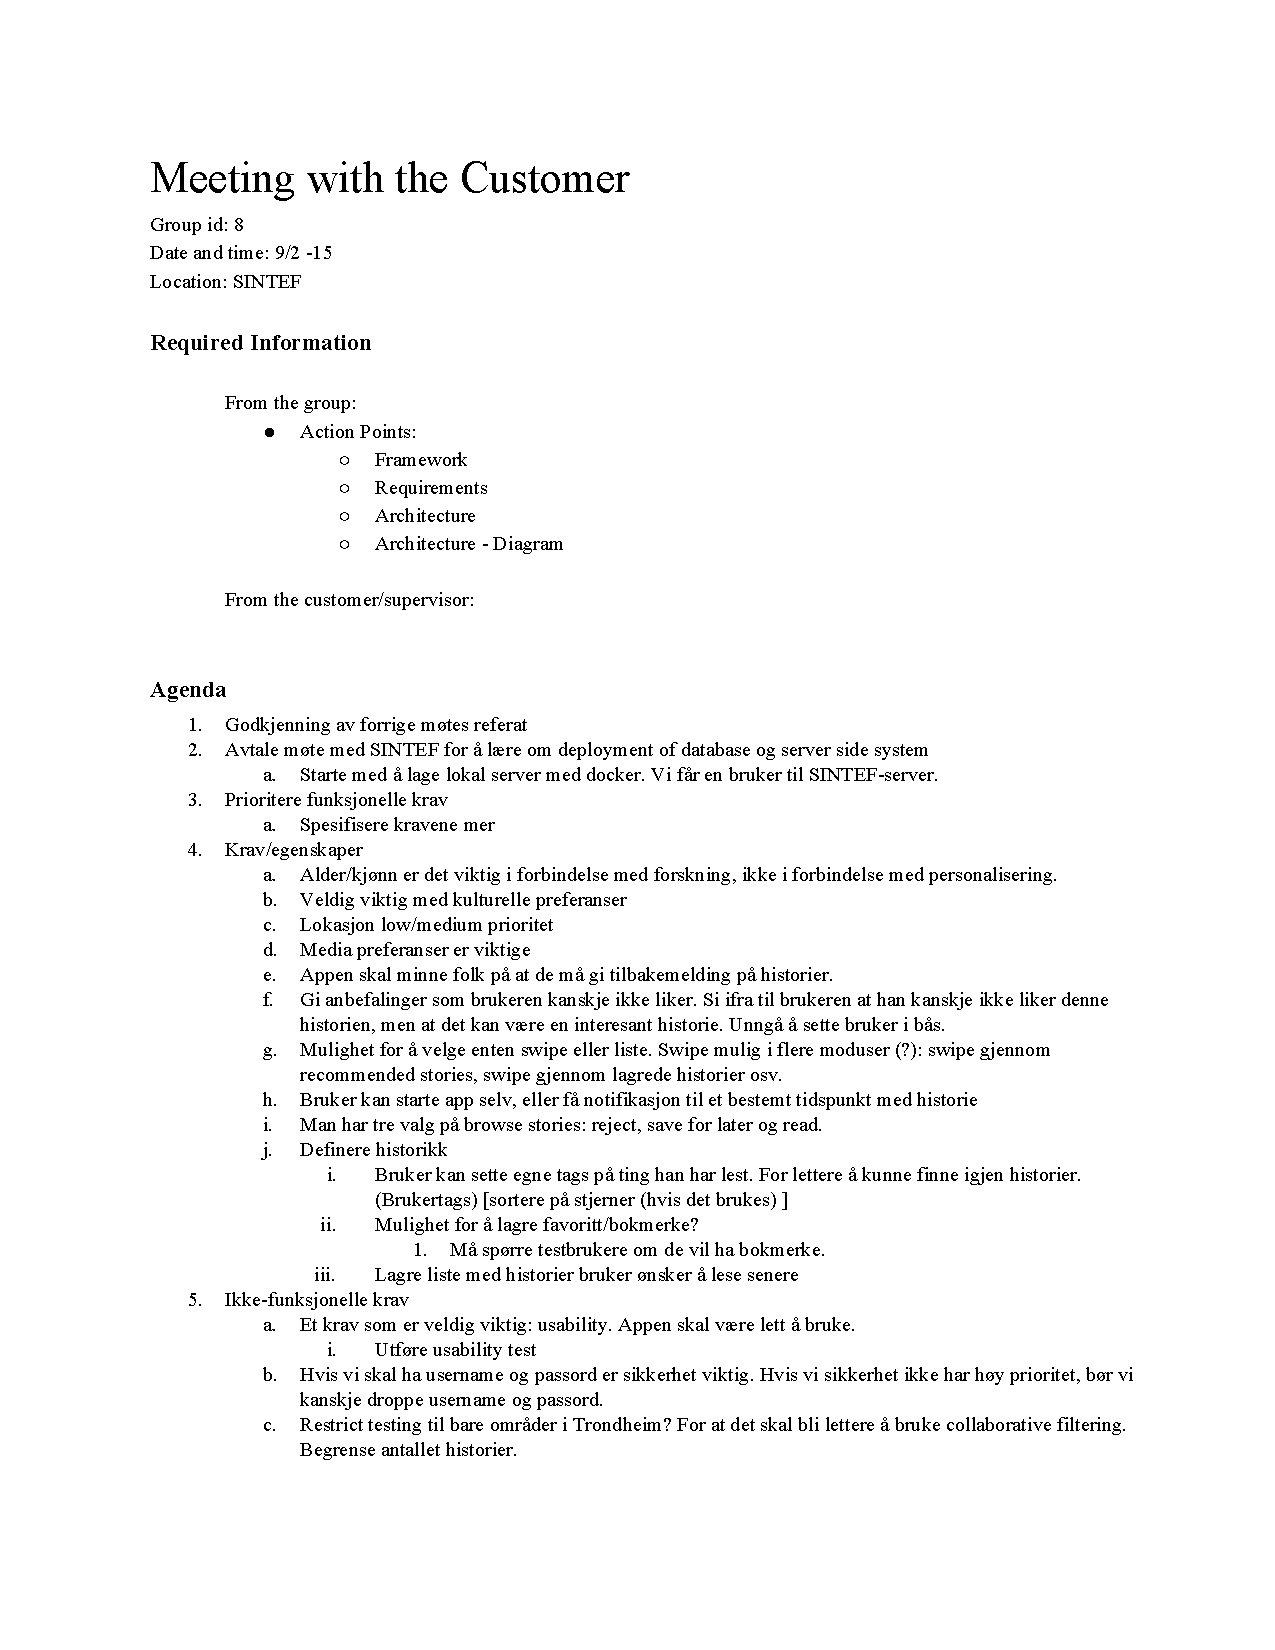
\includepdf[pages=1, pagecommand=\label{app:customer_meeting}]{pdffig/customer_meeting}

\chapter{Developer guide}
\label{app:developer_guide}

\section{Front-end}

\subsection{Dependencies}

\subsubsection{Android}
\begin{itemize}
	\item Android SDK (See the Requirements and Support section at \url{https://cordova.apache.org/docs/en/3.3.0/guide_platforms_android_index.md.html#Android%20Platform%20Guide)}
\end{itemize}

To sign apk file:
\begin{itemize}
	\item Keytool (JDK)
	\item jarsigner (JDK)
	\item zipalign (JDK)
\end{itemize}

\subsubsection{iOS}
Only possible on Mac OSX
\begin{itemize}
	\item Xcode (install from the App Store)
	Minimum required version is Xcode 4.5. More on this at \url{https://cordova.apache.org/docs/en/3.3.0/guide_platforms_ios_index.md.html#iOS%20Platform%20Guide}
\end{itemize}

\subsection{Setup Guide}

\begin{enumerate}
	\item Install NodeJS (\url{https://nodejs.org/download/})
	\item Install Cordova and Ionic (\url{http://ionicframework.com/getting-started/}) 
 		\begin{verbatim}
 			npm install -g cordova ionic
 		\end{verbatim}
	\item Install Gulp (\url{https://github.com/gulpjs/gulp/blob/master/docs/getting-started.md})
		\begin{verbatim}
			npm install -g gulp
		\end{verbatim}
	\item Restore State (Install dependencies)
  		\begin{verbatim}
  			ionic state restore
  		\end{verbatim}
\end{enumerate}
  
\subsection{Testing} 

Use these commands in the root folder of the project to run the application.

\subsubsection{Android}

First run:
	\begin{verbatim}
		ionic build android
	\end{verbatim}
\begin{itemize}
	\item Emulator (Note that the default Android emulator has many problems and is not recommended to use)
		\begin{verbatim}
			ionic emulate android
		\end{verbatim}
	\item Device
		\begin{verbatim}
			ionic run android
		\end{verbatim}
\end{itemize}

Read more about ionic testing here: \url{http://ionicframework.com/docs/guide/testing.html}

\subsubsection{iOS}

First run:
\begin{verbatim}
	ionic build ios
\end{verbatim}

\begin{itemize}
	\item Emulator
		(You need to run this to install the emulator: \verb|npm install -g ios-sim|)
		\begin{verbatim}
			ionic emulate ios
		\end{verbatim}
	\item Device (requires Apple Developer account)
		\begin{verbatim}
			ionic run ios
		\end{verbatim}
	\item Ionic View app

You can install an app on iOS called Ionic view, and test "Vettu Hva?" through it. 
Requires an Ionic user. 

Run: 
\begin{verbatim}
	ionic upload
\end{verbatim}

You will then be asked to enter login information. 

Then it should be possible to download and run in Ionic View. If it for some reason should not appear, click on the eye icon at the top left and enter the ID from the command line. 

More information about Ionic View: \url{http://blog.ionic.io/view-app-is-alive/}

\end{itemize}

\subsubsection{Browser} 

The application requires internet access.
Testing this way is not recommended. The app uses cordova plugins, and these will not work in the browser. 
\begin{itemize}
	\item Both platforms (Android and iOS) in one view
		\begin{verbatim}
			ionic serve --lab
		\end{verbatim}
	\item Single view which can be resized
		\begin{verbatim}
			ionic serve
		\end{verbatim}
\end{itemize}


\subsection{Building}
  
\subsubsection{Android}

\begin{enumerate}
	\item Generate release build
		\begin{verbatim}
  			cordova build --release android
  		\end{verbatim}
	\item Generate key
		\begin{verbatim}
  			keytool -genkey -v -keystore my-release-key.keystore -alias alias_name 
  				-keyalg RSA -keysize 2048 -validity 10000
  		\end{verbatim}
	\item Signing the APK
		\begin{verbatim}
  		jarsigner -verbose -sigalg SHA1withRSA -digestalg SHA1 
  			-keystore my-release-key.keystore HelloWorld-release-unsigned.apk alias_name
  		\end{verbatim}
    Where the AKP is located i.e. \verb|StoryTelling-Frontend\platforms\android\ant-build|
	\item Optimize the APK
		\begin{verbatim}
  			zipalign -v 4 HelloWorld-release-unsigned.apk HelloWorld.apk
  		\end{verbatim} 
  \end{enumerate} 

(These steps are necessary to update the application after you published it the first time) 

PS. Save the keystore file generated in step 2 for further patching.

Read more about publishing Ionic applications on Android here: \url{http://ionicframework.com/docs/guide/publishing.html}

\subsubsection{iOS}
Apple Developer account required. You can open the .xcodeproj project from the platforms/ios folder.\newline 

You need to set up Xcode with your certificates: 
\url{https://developer.apple.com/library/ios/documentation/IDEs/Conceptual/AppDistributionGuide/MaintainingCertificates/MaintainingCertificates.html#//apple_ref/doc/uid/TP40012582-CH31-SW6}\newline

How to distribute the app to test users:
\url{https://developer.apple.com/library/ios/documentation/IDEs/Conceptual/AppDistributionGuide/TestingYouriOSApp/TestingYouriOSApp.html#//apple_ref/doc/uid/TP40012582-CH8-SW1}

\section{Back-end}

\subsection{Dependencies}

\subsubsection{PHP}

Choose between installing and configuring PHP or downloading a development environment with PHP and MySQL.
\begin{itemize}
	\item Install and configure PHP: \url{http://php.net/manual/en/install.php}
	\item Development environment alternatives:
	\begin{itemize}
		\item XAMPP: \url{https://www.apachefriends.org/download.html}
		\item WAMP for windows: \url{http://www.wampserver.com/en/#download-wrapper}
	\end{itemize}
\end{itemize}
	
\subsubsection{MySQL}
\begin{itemize}
	\item MySQL workbench: \url{https://dev.mysql.com/downloads/workbench/}
\end{itemize}
		
\subsubsection{Java}
\begin{itemize}
	\item Download Java Development Kit: \url{http://www.oracle.com/technetwork/java/javase/downloads/jdk8-downloads-2133151.html}
\end{itemize}
			
\subsubsection{Docker}
\begin{itemize}
	\item Docker install: \url{https://docs.docker.com/installation/}
\end{itemize}
				
				
\subsection{Setup Guide}
\begin{enumerate}
	\item Install PHP, MySQL and Java on preferred development device
	\item Install Docker on chosen server
	\item Clone "Vettu hva?" repository:
	\begin{verbatim}
	git clone https://github.com/ewolden/vettu-hva
	\end{verbatim}
	\item Copy config.php and Dockerfile to server.
	\item Define the paramaters in the config.php file:
	\begin{itemize}
		\item DB\_USERNAME - Can be left as root since this is only used internally in the image
		\item DB\_PASSWORD - Can be left blank since this is only used internally in the image
		\item DB\_HOST - Can be left blank which is the same as typing localhost
		\item DB\_NAME - storytelling is the name of the database
		\item API\_URL - This is the URL to digitalt musems API
		\item API\_KEY - The API key needed to use digitalt museums API
		\item APP\_MAIL - The email used for sending users emails upon creation of user (uses a gmail address)
		\item APP\_MAIL\_PASS - The password for the email given
	\end{itemize}
	
	\item Set up docker container on server
	\begin{itemize}
		\item Run the following command to set up a docker container (see more detailed description here: \url{https://github.com/ewolden/vettu-hva}):
		\begin{verbatim}
		docker build -t optional_ImageName folder_with_config_and_dockerfile
		\end{verbatim}
		\item Create a volume for docker to store databases in (only needs to be done the first time):
		\begin{verbatim}
		docker create -v /dbdata --name Storytelling-DBdata optional_imageName
		\end{verbatim}
		\item Start the docker image and from the database storage:
		\begin{verbatim}
		docker run -d --volumes-from vettuhva-DBdata --name vettuhva-backend -p 
		optional_external_port:80 -p optional_external_port:3306 -e 
		MYSQL_PASS="chosen password" optional_imageName
		\end{verbatim}
		\item To stop the running container:
		\begin{verbatim}
		docker stop containerName
		\end{verbatim}
		\item To remove old containers:
		\begin{verbatim}
		docker rm containerName
		\end{verbatim}
	\end{itemize}
\end{enumerate}

\subsection{Testing} 	
Use PHPUnit for testing PHP code. Download and get started with PHPUnit here:  \url{https://phpunit.de/getting-started.html} \newline
Use JUnit for testing Java code. Get started with JUnit here: \url{https://github.com/junit-team/junit/wiki/Getting-started}

\begin{comment}
Occantionally, when testing the controller.php file in the requests folder, a variation of this code have been used:

\begin{verbatim}
	$url = 'serverlocation/requests/controller.php';
	$postarray = json_encode(array('request parameters'));

	$ch = curl_init();
	curl_setopt($ch, CURLOPT_URL, $url);
	
	curl_setopt($ch, CURLOPT_POST, 1);
	curl_setopt($ch, CURLOPT_POSTFIELDS, $postarray);
	//curl_setopt($ch, CURLOPT_RETURNTRANSFER, true);
	//curl_setopt($ch, CURLOPT_HEADER, 0);
	curl_setopt($ch, CURLOPT_HTTPHEADER, array(
	'Content-Type: application/json',
	'Accept: application/json'
	));
	//curl_setopt($ch, CURLOPT_VERBOSE, 1);
	//curl_setopt($ch, CURLOPT_HEADER, 0);
	
	$response = json_decode(curl_exec($ch), true);
	if(curl_errno($ch)) echo 'error:' . curl_error($ch);
	
	curl_close($ch);
	print_r($response);
\end{verbatim}
\end{comment}



\clearpage
\chapter{User manual}
\label{app:user_manual}
This is a guide on how to use the application "Vettu Hva?". It will explain the the basics of how to interact with the app. 


\section{Starting the app}
When opening the app for the first time, an introduction to the app will be displayed. This can be browsed by tapping the "Neste" button. 
\begin{figure}[h!]
		\centering
		\begin{subfigure}[h]{0.32\textwidth}
			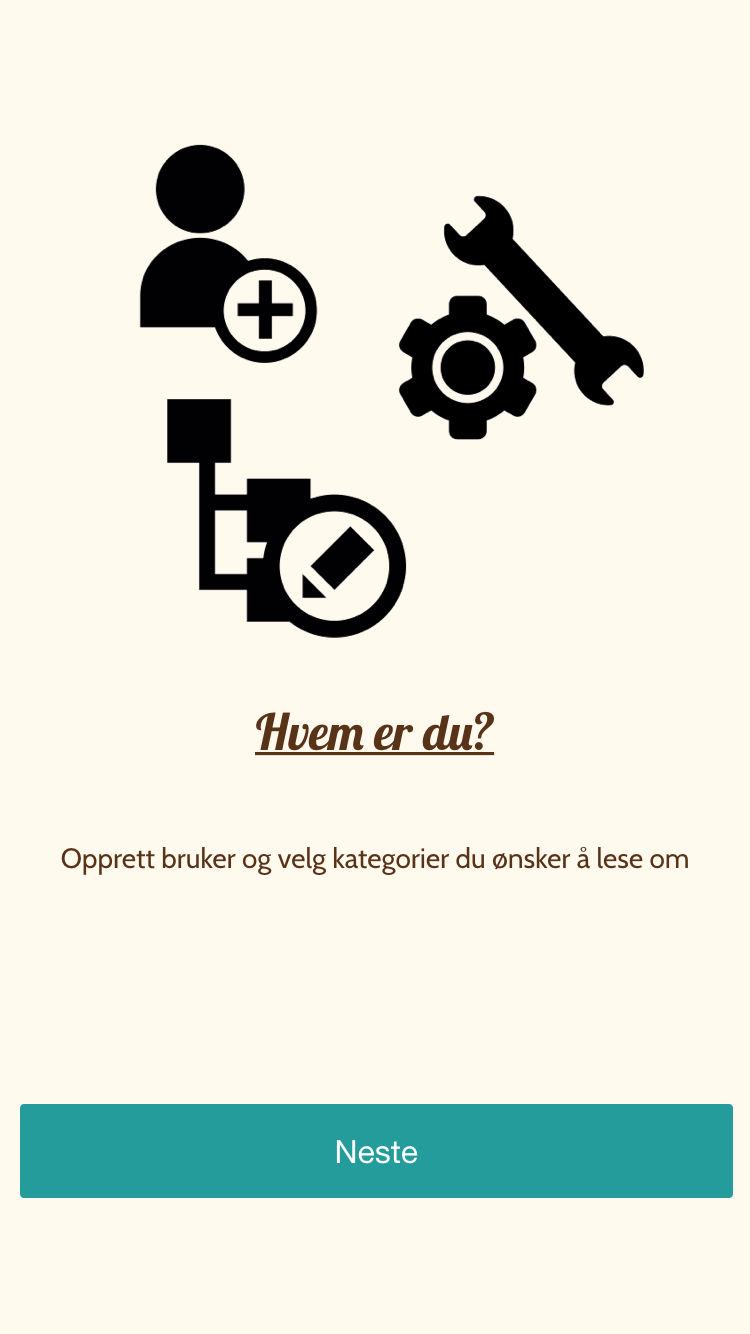
\includegraphics[width=\textwidth]{fig/screenshot_intro1}
			\caption{}
		\end{subfigure}
		\begin{subfigure}[h]{0.32\textwidth}
			
\includegraphics[width=\textwidth]{fig/screenshot_intro2}
			\caption{}
		\end{subfigure}
		\begin{subfigure}[h]{0.32\textwidth}
			
\includegraphics[width=\textwidth]{fig/screenshot_intro3}
			\caption{}
		\end{subfigure}
		\caption{Introduction}
		\label{fig:manual_introduction}
	\end{figure}
\clearpage
After the last of the three introduction screens, the login screen is displayed. There are three choices:
\begin{itemize}
	\item Create a new user by entering an e-mail address that have not been registered in this application before. A confirmation e-mail will be sent to this address. 
	\item Log in to an existing user by entering the e-mail address connected to that user. 
	\item Skip this step by tapping the link towards the bottom of the screen. This means that there is no possibility to log in on another device, and if logging out there is no way to retrieve the information associated with the user. This can be done at a later time in settings by entering an e-mail address. 
\end{itemize}
	If logging in, the main screen will be displayed. Otherwise, the app will additionally ask for profile information (age group and gender) and cultural interests. 


	\begin{figure}[h!]
		\centering
		\begin{subfigure}[h]{0.32\textwidth}
			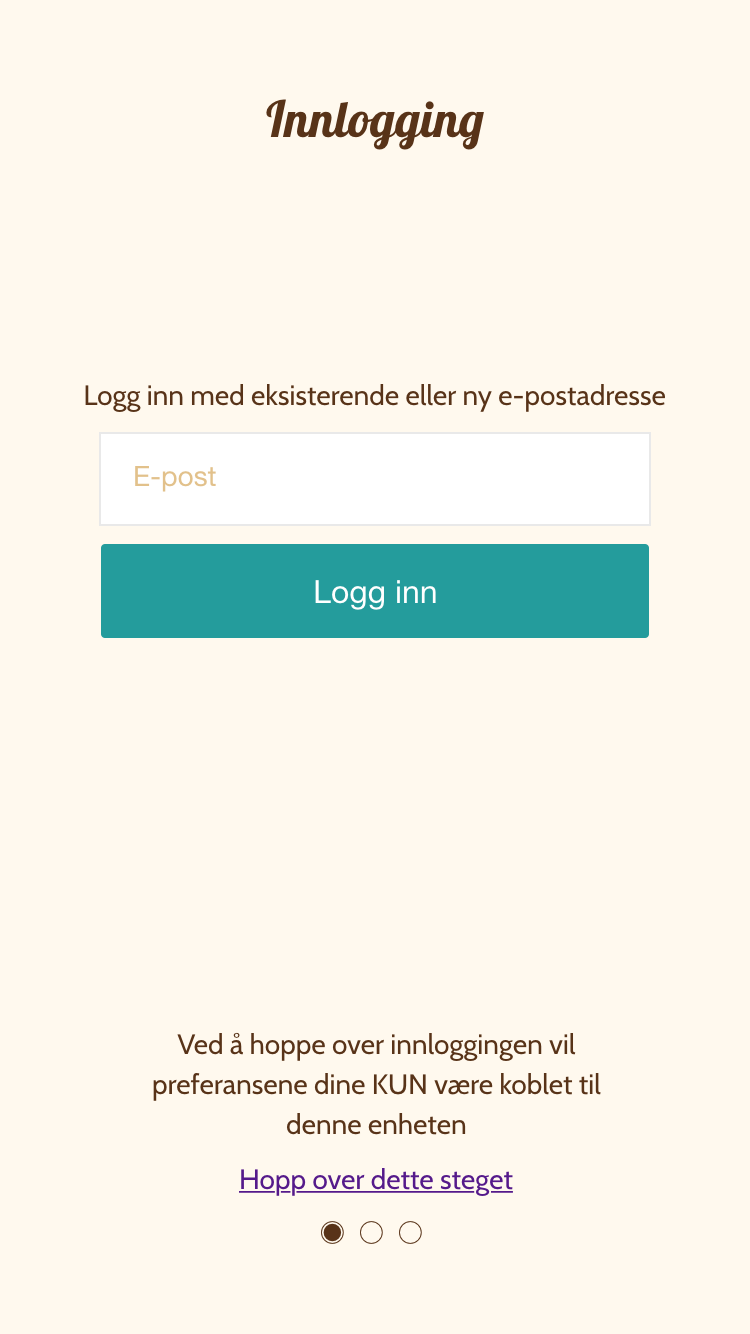
\includegraphics[width=\textwidth]{fig/screenshot_login}
			\caption{Sign in}
		\end{subfigure}
		\begin{subfigure}[h]{0.32\textwidth}
			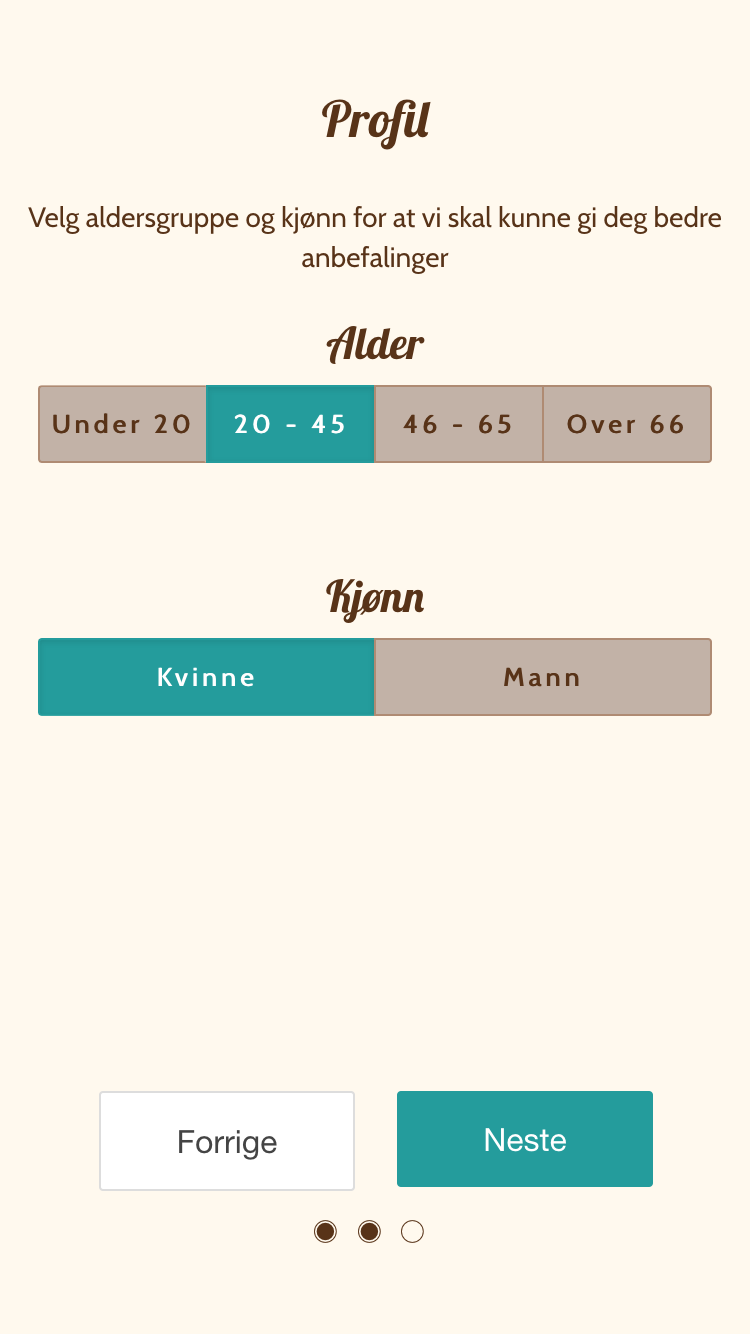
\includegraphics[width=\textwidth]{fig/screenshot_profile}
			\caption{Profile}
		\end{subfigure}
		\begin{subfigure}[h]{0.32\textwidth}
			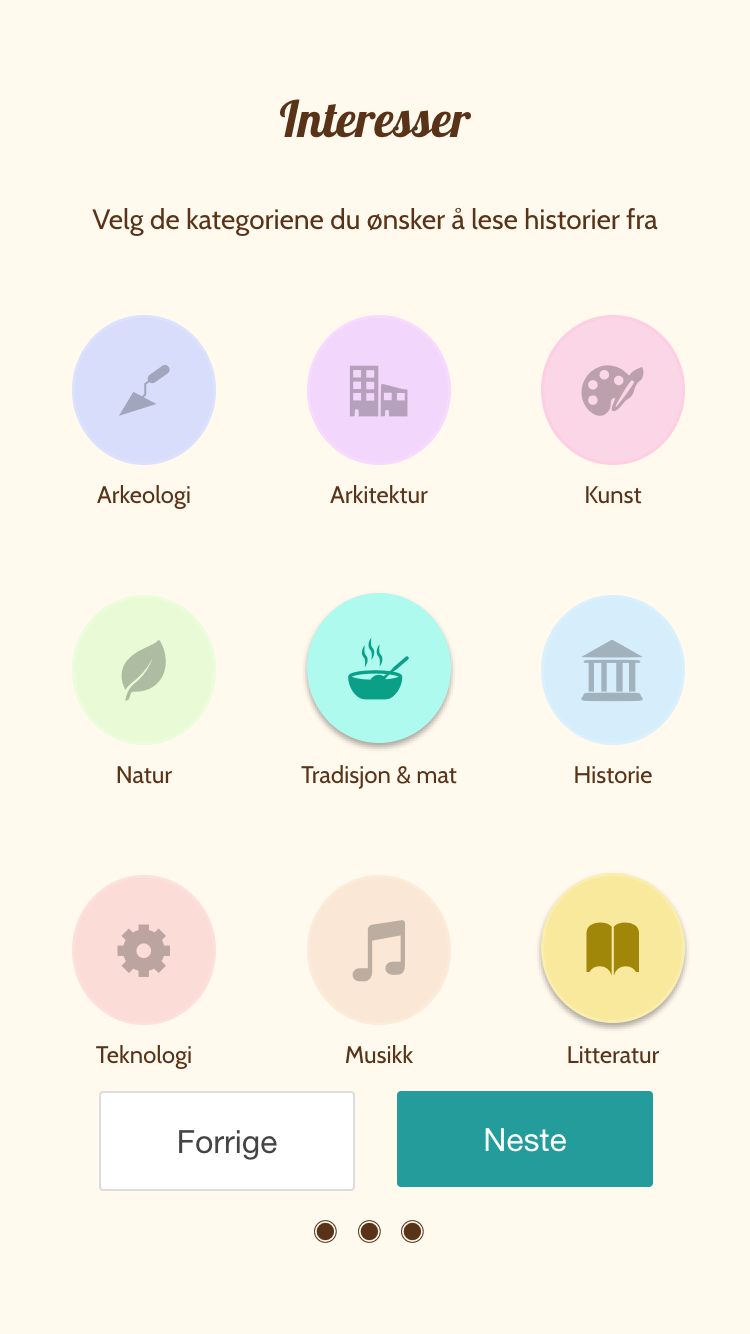
\includegraphics[width=\textwidth]{fig/screenshot_interests}
			\caption{Interests}
		\end{subfigure}
		\caption{Login}
		\label{fig:manual_login}
	\end{figure}

\clearpage
\section{Browsing stories}
Browse stories by swiping left and right or by tapping the arrow buttons on each side. Under the photo of each story are the categories the story belongs to and the media types that the story offers. The text below each card is the explanation of why the story was recommended. This may not appear in the beginning as it will not have any feedback to be based on. Tap a card to read the story.\newline

The detailed view of a story displays text content, images, video, and/or audio. Which media types are available will vary from story to story. Images and video can be viewed in fullscreen, except some videos which are from Youtube or Vimeo which will be opened in the browser.  
\begin{figure}[h!]
		\centering
		\begin{subfigure}[h]{0.32\textwidth}
			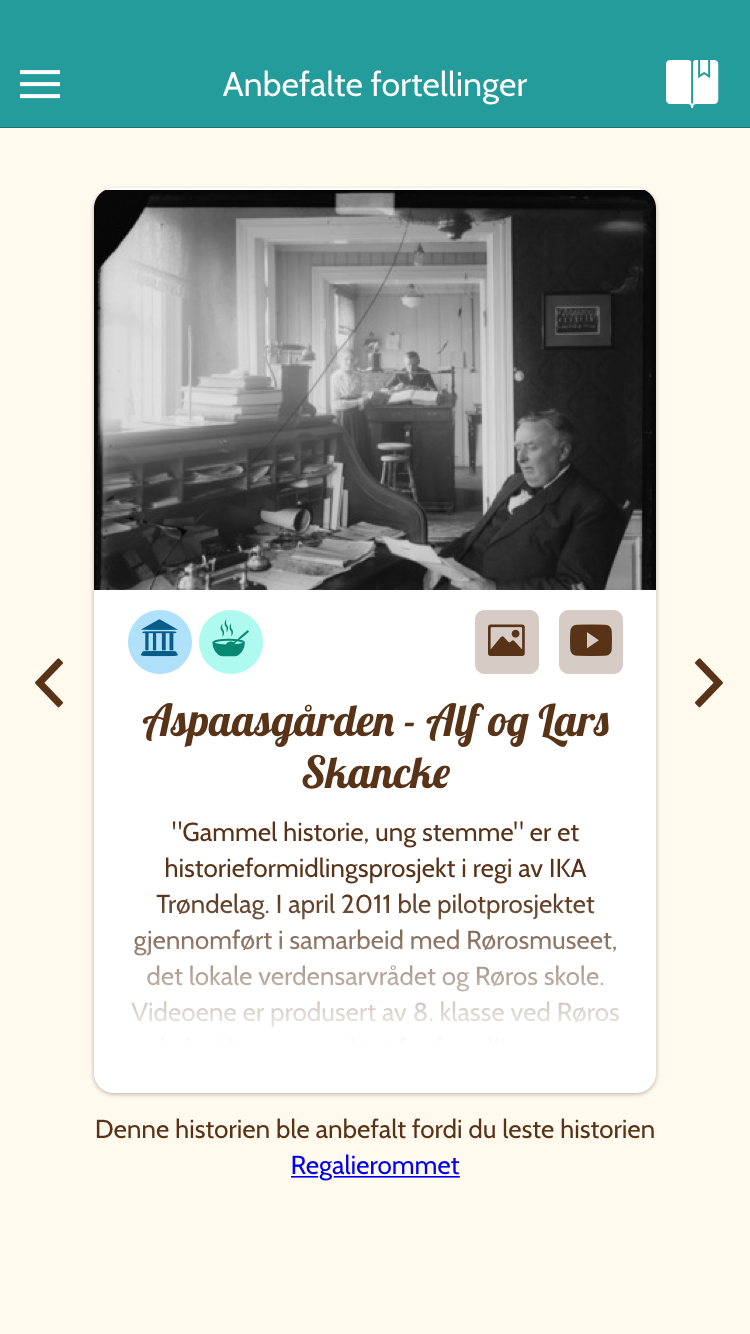
\includegraphics[width=\textwidth]{fig/screenshot_recommendations}
			\caption{Recommended stories}
		\end{subfigure}
		\begin{subfigure}[h]{0.32\textwidth}
			
\includegraphics[width=\textwidth]{fig/screenshot_story}
			\caption{Detailed view of a story}
		\end{subfigure}
		\begin{subfigure}[h]{0.32\textwidth}
			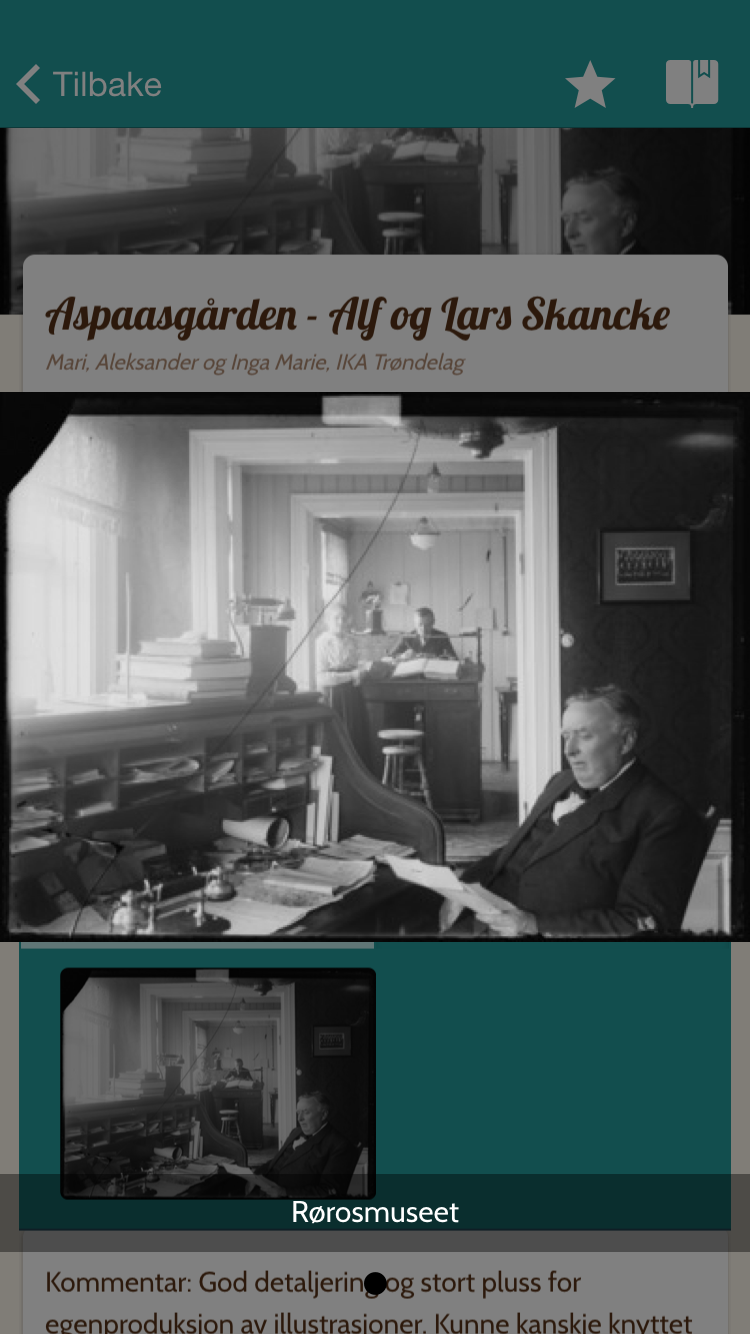
\includegraphics[width=\textwidth]{fig/screenshot_image}
			\caption{Fullscreen image}
		\end{subfigure}
		\caption{Browsing stories}
		\label{fig:manual_browsing}
\end{figure}
\clearpage
\section{Rating a story}
After reading a story, give the app feedback by rating the story. This can be done either by tapping the stars at the bottom of the story, or by doing it in the popup that appears when tapping the star icon in the top bar. This feedback is necessary for the app to provide good story recommendations. 
\begin{figure}[h!]
		\centering
		\begin{subfigure}[h]{0.32\textwidth}
			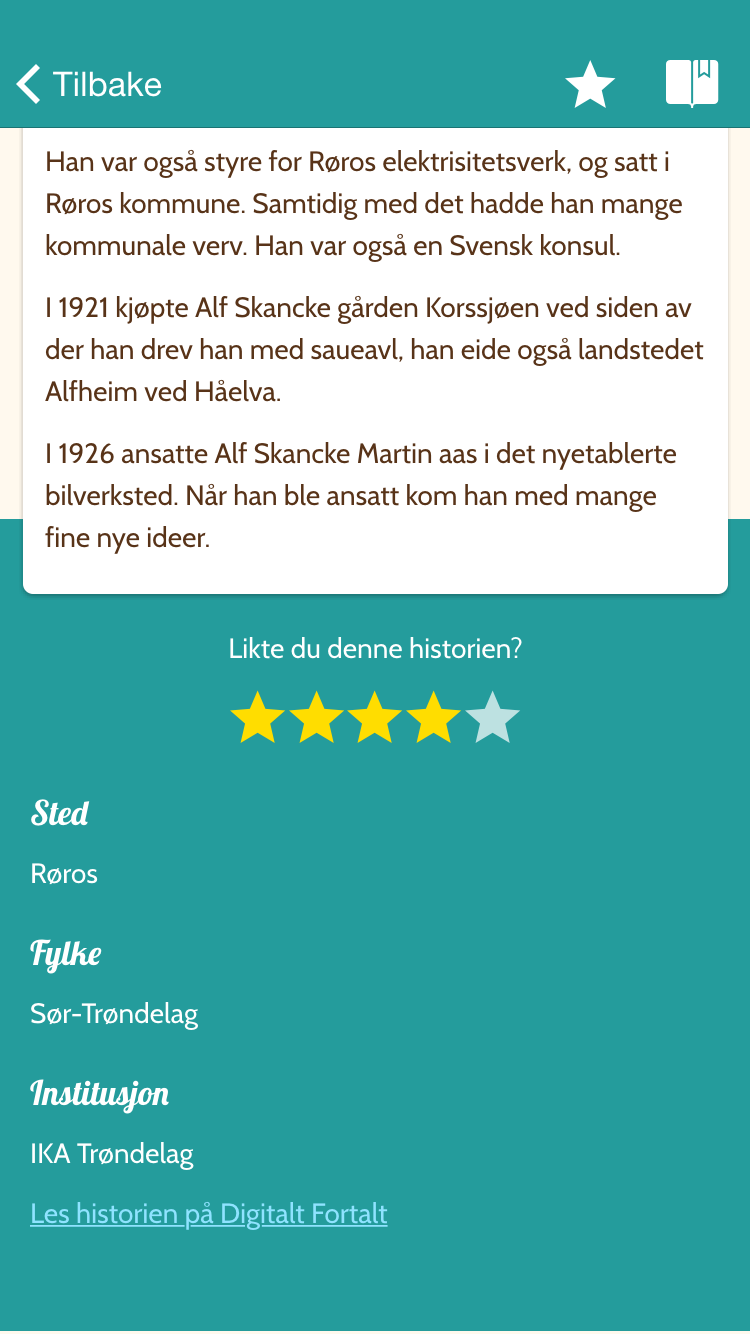
\includegraphics[width=\textwidth]{fig/screenshot_story2}
			\caption{Rating at bottom of a story}
		\end{subfigure}
		\hspace{1cm}
		\begin{subfigure}[h]{0.32\textwidth}
			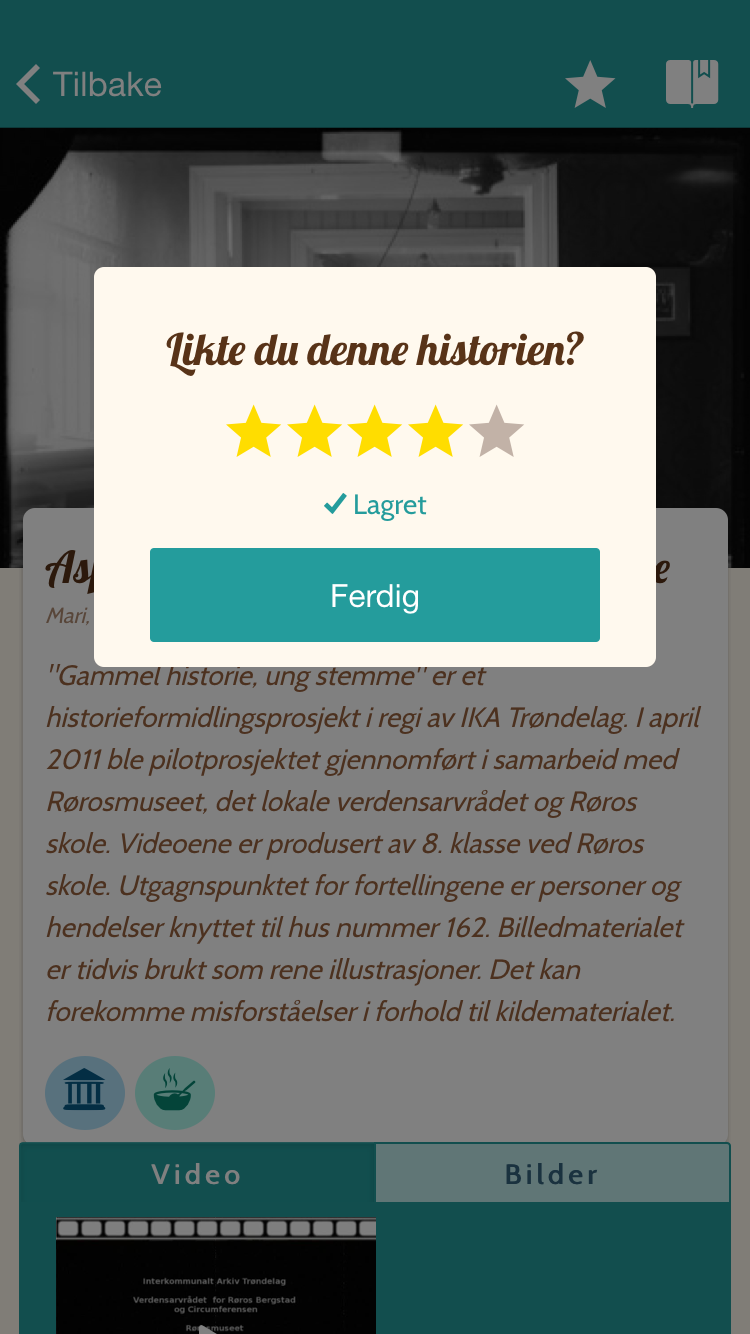
\includegraphics[width=\textwidth]{fig/screenshot_rating}
			\caption{Rating popup}
		\end{subfigure}
		\caption{Rating a story}
		\label{fig:manual_rating}
	\end{figure}

\clearpage
\section{Bookmarks}
To save a story for later bookmarks can be added, both when browsing recommendations and when viewing the details of a story. This is done by tapping the bookmark icon in the top bar. A popup will appear with the predefined "Les senere" list. To create a new bookmark list, you can tap the plus icon and type in a name. The story can then be found later by going into the menu and selecting the list it was saved in. When viewing a list, a story can be removed from it by swiping to the left. To remove an entire list, go to the menu and tap the x-icon on the list to delete. 

\begin{figure}[h!]
		\centering
		\begin{subfigure}[h]{0.3\textwidth}
			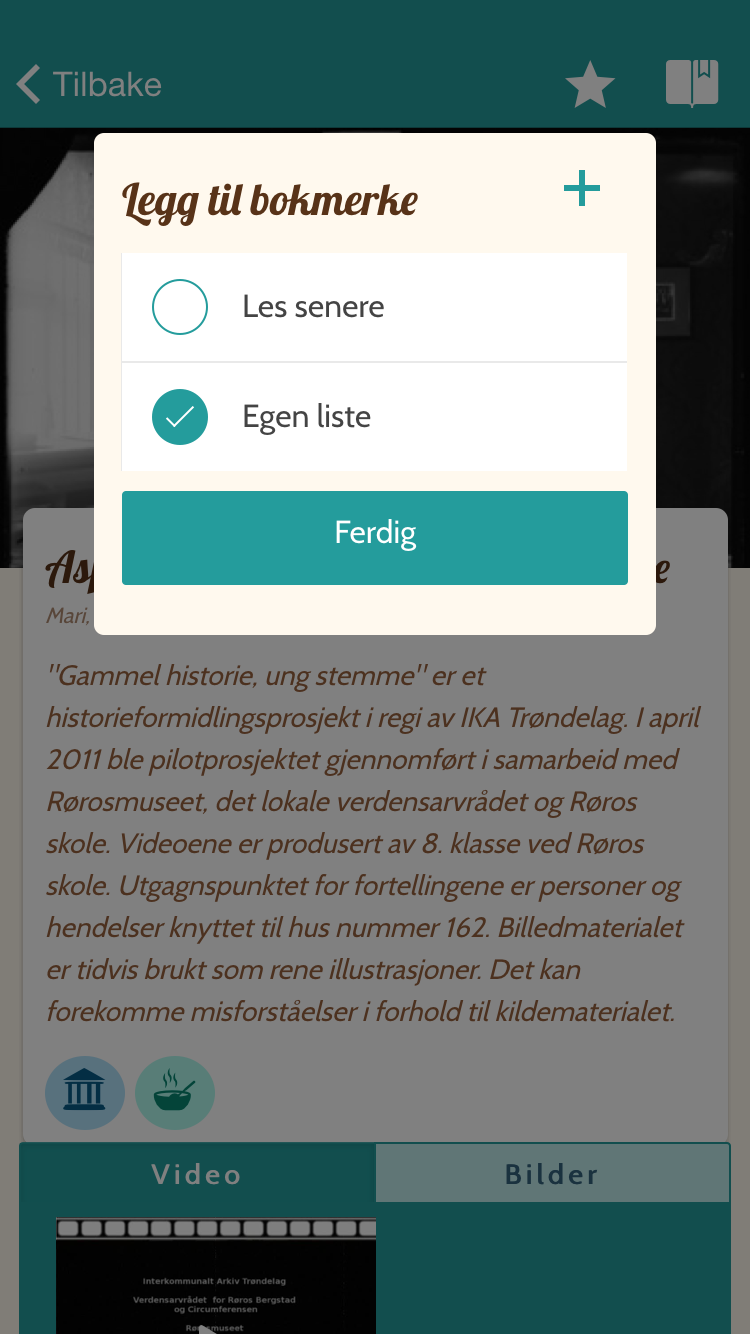
\includegraphics[width=\textwidth]{fig/screenshot_bookmark}
			\caption{Add bookmark}
		\end{subfigure}
		\hspace{1cm}
		\begin{subfigure}[h]{0.3\textwidth}
			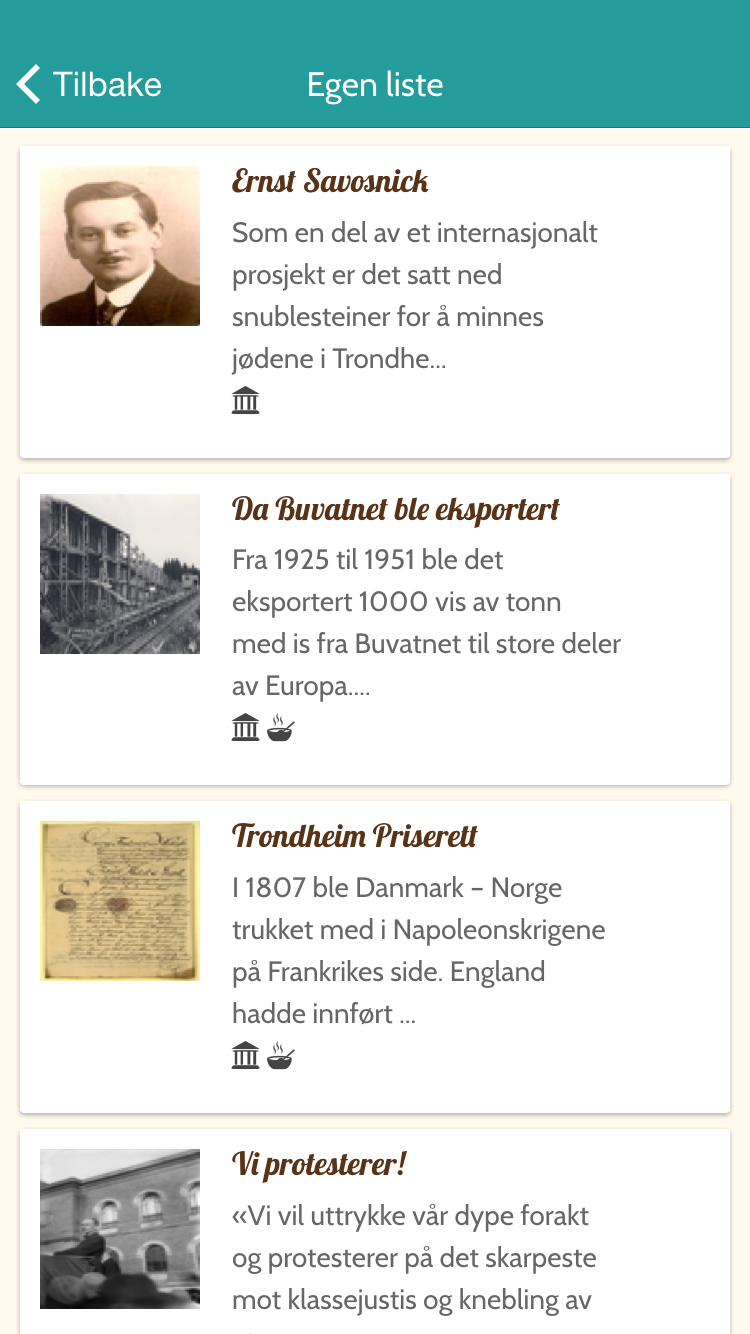
\includegraphics[width=\textwidth]{fig/screenshot_list}
			\caption{Bookmark list}
		\end{subfigure}
		\caption{Bookmarks}
		\label{fig:manual_bookmarks}
	\end{figure}

\clearpage
\section{Other}
From the menu it is possible to view bookmarks, settings, go through the app introduction again or log out. In the settings the email address, profile information and interests can be changed. It also provides more information about the app and the project. 

	
	\begin{figure}[h!]
		\ContinuedFloat
		\centering
		\begin{subfigure}[h]{0.3\textwidth}
			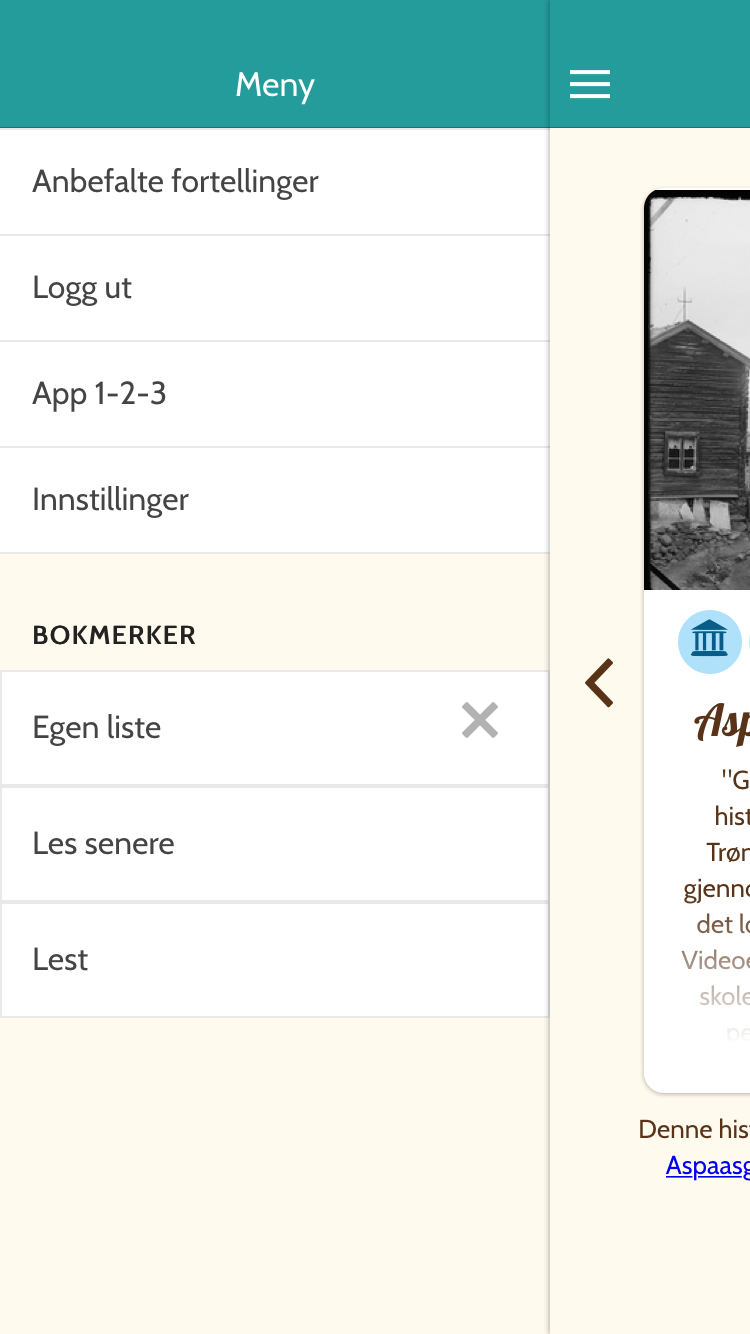
\includegraphics[width=\textwidth]{fig/screenshot_menu}
			\caption{Menu}
		\end{subfigure}
		\hspace{1cm}
		\begin{subfigure}[h]{0.3\textwidth}
			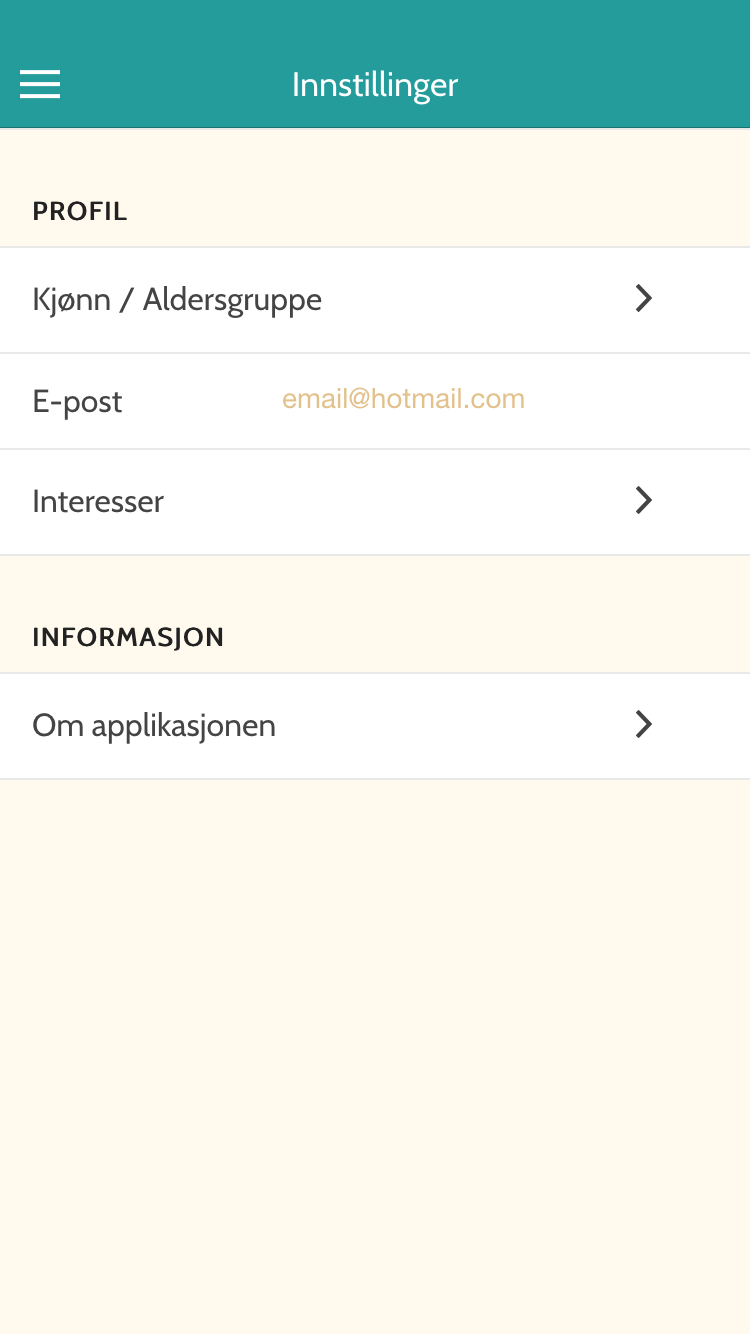
\includegraphics[width=\textwidth]{fig/screenshot_settings}
			\caption{Settings}
		\end{subfigure}
		\label{fig:other}
	\end{figure}

\end{appendices}
\cleardoublepage		%% Optional

\end{document}